\documentclass[oneside,12pt]{book}          % ----- Book

%%%%%%%%%%%%%%%%%%
%%%%% Macros %%%%%
%%%%%%%%%%%%%%%%%%

%%%%%%%%%%%%%%%%%%%%%%%%%%%%
%%%%% Police et langue %%%%%
%%%%%%%%%%%%%%%%%%%%%%%%%%%%

\usepackage[x11names]{xcolor}                           % ----- Couleurs
\usepackage[utf8]{inputenc}                             % ----- UTF-8
\usepackage[french]{babel}                              % ----- French
\usepackage{amsmath,amssymb,mathrsfs}                   % ----- Maths
\usepackage{fontawesome}                                % ----- Caractères / Symboles
\usepackage{eurosym}                                    % ----- Currencies

\usepackage{helvet}										% ----- Police texte
\renewcommand{\familydefault}{\sfdefault}
\usepackage[T1]{fontenc}

\usepackage{mathpazo}									% ----- Police maths


%%%%%%%%%%%%%%%%
%%%%% TikZ %%%%%
%%%%%%%%%%%%%%%%

\usepackage{pgfplots}                                   % ----- Plots
    \pgfplotsset{compat=1.18}
\usepackage{tikz, tikz-3dplot, tkz-tab}                 % ----- TikZ, TikZ 3D, Tableaux
    \usetikzlibrary{math,arrows}                            % ----- Maths, Vecteurs
    \usetikzlibrary{automata, positioning,patterns.meta}    % ----- Graphs
    \usetikzlibrary{decorations.fractals}                   % ----- Fractals


%%%%%%%%%%%%%%%%%%%%
%%%%% Pratique %%%%%
%%%%%%%%%%%%%%%%%%%%

\usepackage[explicit]{titlesec}							% ----- Titres et sections
\usepackage{calc}                                       % ----- Calc / Minipage
\usepackage{fancyhdr}                                   % ----- Header and footer
\usepackage{geometry}                                   % ----- Géométrie de la page
\usepackage{tcolorbox}                                  % ----- Boxes environment
    \tcbuselibrary{skins,listings,listingsutf8}             % ----- All libraries
\usepackage{varwidth}                                   % ----- Adjust box width
\usepackage{fourier-orns}                               % ----- Déco



%%%%%%%%%%%%%%%%%%%%%%%%
%%%%% Mise en page %%%%%
%%%%%%%%%%%%%%%%%%%%%%%%

\usepackage{parskip}									% ----- Parskip
    \setlength{\parskip}{\medskipamount}
    \newcommand{\restoreskip}{\setlength{\parskip}{\medskipamount}}
\geometry{left=30pt, right=30pt, top=55pt, bottom=55pt} % ----- Marges
\setlength\parindent{0mm}                               % ----- No indent
\pagestyle{fancy}                                       % ----- Set-up fancy
\fancyhf[LH]{M. Olivry}                                 % ----- En-tête gauche
\fancyhf[CF]{\footnotesize \copyright ~~  Tous droits réservés ~~ \copyright }        % ----- Copyright
\AtEndDocument{\label{PageFin}}                         % ----- Label dernière page
\fancyhf[RF]{\thepage / \pageref{PageFin}}              % ----- Numéro de page
\setlength{\headheight}{22pt}                           % ----- Adjust head height
\usepackage{setspace}                                   % ----- Interligne
\usepackage{makecell}
\renewcommand{\headrule}{\vspace{-4pt}\hrulefill\raisebox{-2.1pt}{\quad\decofourleft~\decosix~\decofourright \quad}\hrulefill}     % ----- Ornement central

%%%%%%%%%%%%%%%%%%%%%%%%%%%%%%%%%%
%%%%% ----- New colors ----- %%%%%
%%%%%%%%%%%%%%%%%%%%%%%%%%%%%%%%%%

\definecolor{persianblue}{HTML}{221177} % ----- New blues
\definecolor{lightblue}{HTML}{EEFFFF}
\definecolor{softblue}{HTML}{6655BB}

\definecolor{maroon}{HTML}{992222}      % ----- New reds
\definecolor{lightred}{HTML}{FAEEEE}

\definecolor{calgreen}{HTML}{005500}    % ----- New greens
\definecolor{lightgreen}{HTML}{EEFFEE}
\definecolor{softgreen}{HTML}{449944}

\definecolor{brickorange}{HTML}{CC7033} % ----- New oranges
\definecolor{lightorange}{HTML}{FFF2E6}

\definecolor{pinkish}{HTML}{D7AACC}     % ----- Colors for geometry
\definecolor{greenish}{HTML}{AACCBB}
\definecolor{brownish}{HTML}{DDA377}



%%%%%%%%%%%%%%%%%%%%%%%%%%%%%%%%%
%%%%% ----- \theoreme ----- %%%%%
%%%%%%%%%%%%%%%%%%%%%%%%%%%%%%%%%

\newtcolorbox{theorembox}[2][]{% ----- Theorem box
enhanced,
arc=5pt,
frame style = {left color=persianblue , right color=softblue},
colback=lightblue,
fonttitle=\bfseries,
lifted shadow={1mm}{-1.5mm}{2mm}{0.3mm},
hbox,
title={#2},
attach boxed title to top left={xshift=5mm,yshift=-2mm},
boxed title style = {colback = persianblue , colframe = persianblue},
#1}


\newcommand\theoreme[2]{% ----- Theorem command
    \begin{theorembox}[]{\faBook~~#1~~\faBook}
        \begin{varwidth}{\linewidth-15pt }
        #2
        \end{varwidth}
    \end{theorembox}
}



%%%%%%%%%%%%%%%%%%%%%%%%%%%%%%%%%%%
%%%%% ----- \definition ----- %%%%%
%%%%%%%%%%%%%%%%%%%%%%%%%%%%%%%%%%%

\newtcolorbox{definitionbox}[2][]{% ----- Definition box
enhanced,
arc=5pt,
frame style = {left color=calgreen , right color=softgreen},
colback=lightgreen,
fonttitle=\bfseries,
lifted shadow={1mm}{-1.5mm}{2mm}{0.3mm},
hbox,
title={#2},
attach boxed title to top left={xshift=5mm,yshift=-2mm},
boxed title style = {colback = calgreen , colframe =calgreen},
#1}


\newcommand\definition[2]{% ----- Definition command
    \begin{definitionbox}[]{\faUniversity~~#1~~\faUniversity}
        \begin{varwidth}{\linewidth-15pt}
        #2
        \end{varwidth}
    \end{definitionbox}
}



%%%%%%%%%%%%%%%%%%%%%%%%%%%%%%%
%%%%% ----- \astuce ----- %%%%%
%%%%%%%%%%%%%%%%%%%%%%%%%%%%%%%

\newtcolorbox{astucebox}[1][]{% ----- astuce box
enhanced,
arc=10pt,
frame hidden,
borderline={1mm}{0mm}{maroon,dotted},
colback=lightred,
fonttitle=\bfseries,
hbox,
title={\faLightbulbO~~Astuce~~\faLightbulbO},
attach boxed title to top left={xshift=5mm,yshift=-2mm},
boxed title style = {colback = maroon , colframe =maroon},
#1}


\newcommand\astuce[1]{% ----- astuce command
    \begin{astucebox}[]
        \begin{varwidth}{\linewidth-15pt }
        #1
        \end{varwidth}
    \end{astucebox}
}



%%%%%%%%%%%%%%%%%%%%%%%%%%%%%%%%
%%%%% ----- \methode ----- %%%%%
%%%%%%%%%%%%%%%%%%%%%%%%%%%%%%%%

\newtcolorbox{methodebox}[2][]{% ----- methode box
enhanced,
arc=10pt,
frame hidden,
borderline={1mm}{0mm}{maroon,dotted},
colback=lightred,
fonttitle=\bfseries,
hbox,
title={#2},
attach boxed title to top left={xshift=5mm,yshift=-2mm},
boxed title style = {colback = maroon , colframe =maroon},
#1}


\newcommand\methode[2]{% ----- methode command
    \begin{methodebox}[]{\faCogs~~#1~~\faCogs}
        \begin{varwidth}{\linewidth-15pt }
        #2
        \end{varwidth}
    \end{methodebox}
}



%%%%%%%%%%%%%%%%%%%%%%%%%%%%%%%%%%%
%%%%% ----- \exemple ----- %%%%%
%%%%%%%%%%%%%%%%%%%%%%%%%%%%%%%%%%%

\newtcolorbox{exemplebox}[1][]{% ----- exemple box
enhanced,
frame hidden,
borderline west={2pt}{0pt}{brickorange},
%borderline south={2pt}{0pt}{brickorange},
interior style = {top color = lightorange , bottom color = white},
fonttitle=\bfseries,
hbox,
#1}


\newcommand\exemple[2]{% ----- exemple command
    \begin{exemplebox}[]
        \begin{varwidth}{\linewidth-15pt }
        \textbf{\underline{Exemple}:} \\[5pt]
        #1
        \end{varwidth}
    \end{exemplebox}
}

%%%%%%%%%%%%%%%%%%%%
%%% Mise en page %%%
%%%%%%%%%%%%%%%%%%%%

\newcommand\titre[1]{\begin{center} \textbf{\LARGE #1} \end{center}}

\newcommand*\circled[1]{\tikz[baseline=(char.base)]{
            \node[shape=circle,draw,inner sep=2pt] (char) {#1};}}

            
%%%%%%%%%%%%%%%%%%
%%%% Ensembles %%%
%%%%%%%%%%%%%%%%%%

\newcommand\CC{%
        {\mathbb C}} % ----- Ensemble C

\newcommand\RR{%
        {\mathbb R}} % ----- Ensemble R

\newcommand\QQ{%
        {\mathbb Q}} % ----- Ensemble Q

\newcommand\ZZ{%
        {\mathbb Z}} % ----- Ensemble Z

\newcommand\NN{%
        {\mathbb N}} % ----- Ensemble N

\newcommand\PP{%
        {\mathbb P}} % ----- P probas

\newcommand\EE{%
        {\mathbb E}} % ----- E espérance

\newcommand\VV{%
        {\mathbb V}} % ----- V variance


\newcommand\nN{%
        {n\in\mathbb N}} % ----- n dans N

\newcommand\xR{%
        {x\in\mathbb R}} % ----- x dans R

\newcommand\zC{%
        {z\in\mathbb C}} % ----- z dans C


%%%%%%%%%%%%%%%%
%%% Symboles %%%
%%%%%%%%%%%%%%%%

\newcommand\dur{%
        {(\star)}} % ----- Exo difficile



\newcommand\limx{%
        {\lim\limits_{x\to +\infty}}\,} % ----- Limite x en plus infini

\newcommand\limn{%
        {\lim\limits_{n\to +\infty}}\,} % ----- Limite n en plus infini

\newcommand\limite[1]{%
        {\lim\limits_{\substack{#1}}}\,} % ----- Limite X verx Y

\newcommand\Ccal{%
        {\mathscr{C}}} % ----- C calligraphique

\newcommand\Dcal{%
        {\mathscr{D}}} % ----- D calligraphique

\newcommand\Pcal{%
        {\mathscr{P}}} % ----- P calligraphique

\newcommand\Rcal{%
        {\mathscr{R}}} % ----- R calligraphique

\newcommand\Fcal{%
        {\mathscr{F}}} % ----- F calligraphique

\newcommand\Scal{%
        {\mathscr{S}}} % ----- S calligraphique

\newcommand\Acal{%
        {\mathscr{A}}} % ----- A calligraphique

\newcommand\Vcal{%
        {\mathscr{V}}} % ----- V calligraphique



%%%%%%%%%%%%%%%%%%%%%%%%%
%%% Accolade à gauche %%%
%%%%%%%%%%%%%%%%%%%%%%%%%

\newcommand{\accol}[1]{%
    {\left\{
    \renewcommand{\arraystretch}{0.8}
    \begin{array}{l}
        #1
    \end{array}
    \right. }}


\newcommand{\accolsized}[2]{%
    {\left\{
    \renewcommand{\arraystretch}{#2}
    \begin{array}{l}
        #1
    \end{array}
    \right. }}



%%%%%%%%%%%%%%%%%%%%%%
%%% Calculs usuels %%%
%%%%%%%%%%%%%%%%%%%%%%

\newcommand\somme[2]{%
        {\displaystyle\sum_{#1}^{#2}}}    % ----- Somme

\newcommand\sommek[2]{%
        {\displaystyle\sum_{k=#1}^{#2}}}    % ----- Somme k

\newcommand\inte[2]{%
        {\displaystyle\int_{#1}^{#2}}}   % ----- Intégrale

\newcommand\dd{%
        {\,\,\mathrm{d}}}       % ----- d différentiel

\newcommand\floor[1]{%
        {\lfloor #1 \rfloor}}   % ----- Floor

\newcommand\ceil[1]{%
        {\lceil #1 \rceil}}     % ----- Ceiling

\newcommand\abs[1]{%
        {\left\lvert #1 \right\rvert}}     % ----- Absolute value
        
\newcommand\pgcd{%
        {\mathrm{pgcd}}}       % ----- pgcd

\newcommand\ppcm{%
        {\mathrm{ppcm}}}       % ----- ppcm




%%%%%%%%%%%%%%
%%% Suites %%%
%%%%%%%%%%%%%%

\newcommand{\defsuite}[2]{%
    \renewcommand{\arraystretch}{0.8}
    \begin{cases}
        #1 \\
        u_{n+1}= #2 \\
    \end{cases}
    }                   % ----- Définition d'une suite (Un) par récurrence

\newcommand\Un{%
        {(u_{n})_{n\in\mathbb N}}} % ----- (Un)_n in N



%%%%%%%%%%%%%%%%%
%%% Géométrie %%%
%%%%%%%%%%%%%%%%%

\newcommand\vvec[1]{\vbox{\halign{##\cr\tiny\textbf{\rightarrowfill}\cr\noalign{\nointerlineskip\vskip2pt}$#1\mskip2mu$\cr}}} % ----- Vecteur

\newcommand\vcoord[2]{\renewcommand{\arraystretch}{0.6}\vvec{#1}\hspace{-2pt}\matrice{#2}} % ----- Coordonnées vecteur

\newcommand\Oij{\left(O\,;\,\vvec{i}\,;\,\vvec{j}\right)} % ----- (O;i;j)

\def\Oijk{\left(O\,;\,\Vec{i}\,;\,\Vec{j}\,;\,\Vec{k}\right)} % ---- (O;i;j;k)

\newcommand\norme[1]{%
        {\left\lVert #1 \right\rVert}}     % ----- Norme

\newcommand\normev[1]{%
        {\left\lVert \vvec{#1} \right\rVert}}     % ----- Norme vecteur

\newcommand\scal[2]{%
    {\vvec{#1}\cdot\vvec{#2}}} % ----- Produit scalaire



%%%%%%%%%%%%%%%%%%%%
%%% Probabilités %%%
%%%%%%%%%%%%%%%%%%%%

\newcommand\barre[1]{%
    {\overline{#1}}} % ----- A barre



%%%%%%%%%%%%%%%%%%%%%%%%%
%%% Nombres complexes %%%
%%%%%%%%%%%%%%%%%%%%%%%%%

\newcommand\Ouv{(O\,;\,\vvec{u}\,;\,\vvec{v})} % ----- (O;u;v)


\newcommand\Reel{%
    {\mathfrak{Re}}} % ----- Partie réelle

\newcommand\Imag{%
    {\mathfrak{Im}}} % ----- Partie imaginaire

\newcommand{\defsuitez}[2]{%
    {\left \{
    \renewcommand{\arraystretch}{0.7}
    \begin{array}{l}
        #1 \\
        z_{n+1}= #2 \\
    \end{array}
    \right. }} % ----- Définition d'une suite complexe (Zn)n par récurrence



%%%%%%%%%%%%%%%%
%%% Matrices %%%
%%%%%%%%%%%%%%%%

\newcommand\matrice[1]{{%
    \renewcommand{\arraystretch}{0.7}
    \arraycolsep=0.7\arraycolsep\ensuremath{\begin{pmatrix}#1\end{pmatrix}}}}


% Packages TikZ / PGF

\usepackage{pgfplots}   % ----- Plots
\pgfplotsset{compat=1.18}
\usepackage{tikz, tikz-3dplot, tkz-tab} % ----- TikZ, TikZ 3D, Tableaux
\usetikzlibrary{math,arrows} % ----- Maths, Vecteurs
\usetikzlibrary{automata, positioning,patterns.meta} % ---- Graphs
\usepackage{calc}


% ----- Création pattern "hatch"

\pgfdeclarepattern{
  name=hatch,
  parameters={\hatchsize,\hatchangle,\hatchlinewidth},
  bottom left={\pgfpoint{-.1pt}{-.1pt}},
  top right={\pgfpoint{\hatchsize+.1pt}{\hatchsize+.1pt}},
  tile size={\pgfpoint{\hatchsize}{\hatchsize}},
  tile transformation={\pgftransformrotate{\hatchangle}},
  code={
    \pgfsetlinewidth{\hatchlinewidth}
    \pgfpathmoveto{\pgfpoint{-.1pt}{-.1pt}}
    \pgfpathlineto{\pgfpoint{\hatchsize+.1pt}{\hatchsize+.1pt}}
    \pgfpathmoveto{\pgfpoint{-.1pt}{\hatchsize+.1pt}}
    \pgfpathlineto{\pgfpoint{\hatchsize+.1pt}{-.1pt}}
    \pgfusepath{stroke}
  }
}
\tikzset{
  hatch size/.store in=\hatchsize,
  hatch angle/.store in=\hatchangle,
  hatch line width/.store in=\hatchlinewidth,
  hatch size=5pt,
  hatch angle=0pt,
  hatch line width=.5pt,
}


% ----- Création pattern "stripe"

\pgfdeclarepattern{
  name=stripe,
  parameters={\stripesize,\stripeangle,\stripelinewidth},
  bottom left={\pgfpoint{-.1pt}{-.1pt}},
  top right={\pgfpoint{\stripesize+.1pt}{\stripesize+.1pt}},
  tile size={\pgfpoint{\stripesize}{\stripesize}},
  tile transformation={\pgftransformrotate{\stripeangle}},
  code={
    \pgfsetlinewidth{\stripelinewidth}
    \pgfpathmoveto{\pgfpoint{-.1pt}{-.1pt}}
    \pgfpathlineto{\pgfpoint{\stripesize+.1pt}{\stripesize+.1pt}}
    \pgfusepath{stroke}
  }
}
\tikzset{
  stripe size/.store in=\stripesize,
  stripe angle/.store in=\stripeangle,
  stripe line width/.store in=\stripelinewidth,
  stripe size=5pt,
  stripe angle=0pt,
  stripe line width=.5pt,
}


%%%%%%%%%%%%%%%%%%%%
%%%%% Sommaire %%%%%
%%%%%%%%%%%%%%%%%%%%

\setcounter{tocdepth}{1}			                    % ----- Table of contents
\usepackage{hyperref}
\hypersetup{colorlinks,citecolor=black,filecolor=black,linkcolor=black,urlcolor=black}


%%%%%%%%%%%%%%%%%%%%%%%%
%%%%% Mise en page %%%%%
%%%%%%%%%%%%%%%%%%%%%%%%

\fancyhf[RH]{T\up{ale} spé.}                            	% ----- En-tête droit
\fancyhead[C]{\hyperlink{sommaire}{\nouppercase\leftmark}}	% ----- En-tête central
\usepackage{setspace}                                   	% ----- Interligne
    \setstretch{1.05}
\usepackage{JeuxCartes}                                 	% ----- Poker


%%%%%%%%%%%%%%%%%%%%%%%%%%%%
%%%%% Corrigé des exos %%%%%
%%%%%%%%%%%%%%%%%%%%%%%%%%%%

\usepackage{answers}
\Newassociation{sol}{Solution}{ans}
\Newassociation{hint}{Indication}{ans}


\renewenvironment{Solution}[2]{%
    \tcbox[size=title,sharp corners,colframe=red!65!black,boxrule=0.8mm,colback=red!20!white]
        {\hyperlink{subsection.#1}{\textbf{#1 - Solution}}} #2}\hrule


\renewenvironment{Indication}[2]{%
    \tcbox[enhanced,size=title,boxrule=0.8mm,colframe=white,borderline={0.8mm}{0mm}{blue!65!black,dashed},colback=white!85!blue]
        {\hyperlink{subsection.#1}{\textbf{#1} - Indications}} #2}


%%%%%%%%%%%%%%%%%%%%%%%%%%%%%%%%%%%%%%%%%%%%%%%%%%%%%%%%%%%%%%%%%%%%%%%%%%%%%%%%%%%%%%%%%%%%%%%%%%%%%%%%%%%
%%%%%%%%%%%%%%%%%%%%%%%%%%%%%%%%%%%%%%%%%%%%%%%%%%%%%%%%%%%%%%%%%%%%%%%%%%%%%%%%%%%%%%%%%%%%%%%%%%%%%%%%%%%
%%%%%%%%%%%%%%%%%%%%%%%%%%%%%%%%%%%%%%%%%%%%%%%%%%%%%%%%%%%%%%%%%%%%%%%%%%%%%%%%%%%%%%%%%%%%%%%%%%%%%%%%%%%
%%%%%%%%%%%%%%%%%%%%%%%%%%%%%%%%%%%%%%%%%%%%%%%%%%%%%%%%%%%%%%%%%%%%%%%%%%%%%%%%%%%%%%%%%%%%%%%%%%%%%%%%%%%
%%%%%%%%%%%%%%%%%%%%%%%%%%%%%%%%%%%%%%%%%%%%%%%%%%%%%%%%%%%%%%%%%%%%%%%%%%%%%%%%%%%%%%%%%%%%%%%%%%%%%%%%%%%

\begin{document}

\begin{titlepage}
\begin{tikzpicture}[remember picture,overlay]
	\draw (0,0) (\paperwidth,\paperheight);

	\node[opacity=0.5,inner sep=0pt] at (current page.center)			{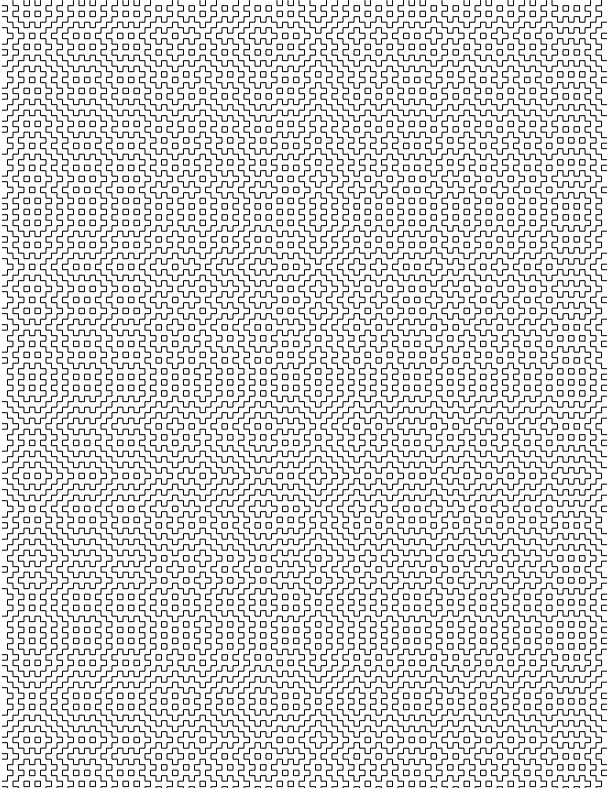
\includegraphics[width=\paperwidth,height=\paperheight]{random_rectangles.png}};

    \node[rounded corners = 8pt, rectangle, inner sep=10pt, fill=white, yshift=8cm] at (current page.center)
              {\makecell{\bfseries\fontsize{40}{60}\selectfont Terminale générale\\[5pt] \bfseries\fontsize{40}{60}\selectfont Spécialité mathématiques}};
	
	\node[rounded corners = 8pt, rectangle, inner sep=10pt, fill=white, yshift=4cm] at (current page.center)
              {\huge\bfseries Livret d'exercices};

	\node[rounded corners = 8pt, rectangle, inner sep=10pt, fill=white, yshift=3cm] at (current page.center)
              {\large\bfseries 2024-2025};
              
	\node[yshift=-4.5cm] at (current page.center) {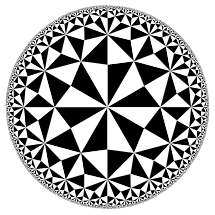
\includegraphics[scale=1]{tessellation.png}};
              
	\node[rounded corners = 8pt, rectangle, inner sep=5pt, fill=white, yshift=-12cm] at (current page.center)
              {\large\bfseries Merlin Olivry};  
\end{tikzpicture}
\end{titlepage}

\renewcommand{\contentsname}{Sommaire}
\hypertarget{sommaire}{}
\tableofcontents
\newpage


\chapter*{Préface}

Chers élèves,

Je suis ravi de vous présenter ce livret d'exercices spécialement conçu pour vous accompagner dans votre parcours en classe de terminale générale avec spécialité mathématiques.\\
Cela fait plusieurs années que j'enseigne les mathématiques, et j'ai souhaité vous offrir un outil complémentaire aux exercices classiques et parfois répétitifs abordés en classe.

\begin{minipage}{0.59\linewidth}
Je précise que je ne prétends à aucune exclusivité quant aux exercices recensés : un exercice ne peut appartenir à personne et vous en trouverez dans ce livret qui sont librement inspirés de sujets de baccalauréats ou d'exercices créés par mes collègues. Mon objectif est avant tout de vous offrir un recueil utile et stimulant pour approfondir vos connaissances.\\

Je revendique cependant la propriété intellectuelle de ce livret en tant que collection d'exercices rédigée et mise en page par mes soins, et toute reproduction devra faire l'objet d'une demande préalable.
\end{minipage}
\begin{minipage}{0.4\linewidth}
\begin{center}
{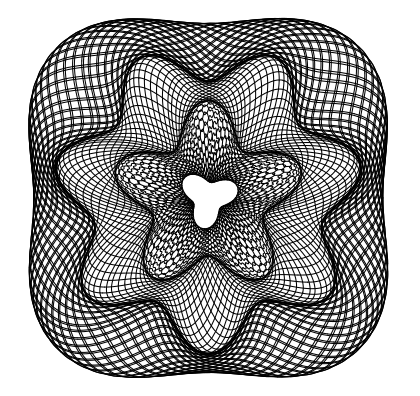
\includegraphics[scale=1]{guilloche.png}}
\end{center}
\end{minipage}


Ce livret est organisé de manière classique par chapitres et sections dans un ordre qui, bien que ne correspondant probablement pas à celui que vous suivrez en classe, me paraît parfaitement adapté à l'année de terminale.

J'ai tenté d'ordonner les exercices par ordre croissant de difficulté au sein de chaque section, même si ce classement n'est pas toujours des plus précis. Vous trouverez ainsi des exercices adaptés à différents niveaux, vous permettant de vous exercer en fonction de vos besoin et des défis que vous souhaitez relever.

N’hésitez pas à aborder les exercices avec une attitude exploratoire, car la difficulté n’est pas toujours indiquée et chaque exercice a son propre degré de complexité et demande des initiatives spécifiques.

Je tiens à souligner que ce livret est destiné à être un complément à vos études et non un substitut aux exercices traités en classe. Il a pour but de consolider vos acquis et à parfaire votre maîtrise du programme.

Ne soyez pas découragés si certains exercices vous semblent particulièrement difficiles ; cela ne reflète en aucun cas une incapacité à comprendre le chapitre en question. La persévérance est une clé essentielle pour votre succès, et l'échec fait partie de l'apprentissage.\\

\begin{minipage}{0.4\linewidth}
\begin{center}
{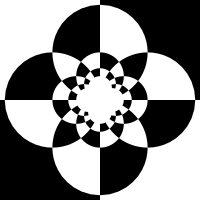
\includegraphics[scale=0.9]{inverse_checker.png}}
\end{center}
\end{minipage}\hfill
\begin{minipage}{0.6\linewidth}
Actuellement, les corrigés des exercices ne sont pas encore disponibles, mais je travaille activement à leur rédaction et je m'efforcerai de les intégrer dans les plus brefs délais.\\
De plus, ce livret est en constante évolution : je prévois d’enrichir son contenu au fil du temps pour mieux répondre à vos besoins et à ceux d'élèves futurs.\\

Je remercie chaleureusement mes élèves qui, chaque jour, résolvent de plus en plus d'exercices et me donnent l'envie de leur en offrir davantage.\\[5pt]
Je tiens à créditer l'ensemble des personnes ayant participé à la lecture, la relecture et la correction de ce livret :
\end{minipage}

\begin{tabular}{p{0.24\linewidth}p{0.24\linewidth}p{0.24\linewidth}p{0.24\linewidth}}
	Jonathan Miron & Victoire Pilon & Hippolyte Besson & Raphaël Picard\\
	Aurore Lorne & Héloïse Bacar-Konig & Lyna Hamadi & Sarah Jenhani\\
	Marion Avril-Laporte & Estelle Petit & Thomas Simoes
\end{tabular}

Je vous souhaite une excellente utilisation de ce livret et une réussite éclatante dans vos études.\\
Que votre curiosité et vos efforts vous mènent vers de nouveaux horizons mathématiques passionnants !

\vspace{85mm}

Les exercices et questions marquées du symbole $\dur$ sont d'une difficulté supérieure aux attendus de cette année.\\
Les question marquées du symbole \faCalculator~ demandent une réponse aidée par une calculatrice.

Si vous remarquez une coquille ou une erreur, que vous voulez proposer une suggestion d'amélioration ou un nouvel exercice, ou pour toute prise de contact, n'hésitez pas à me contacter à l'adresse
\begin{center}\texttt{merlin.olivry.34@gmail.com}\end{center}

Dernière modification le \today.


%%%%%%%%%%%%%%%%%%%%%%%%%%%%%%%%%%%%%%%%%%%%%%%%%%%%%%%%%%%%%%%%%%%%%%%%%%%%%%%%%%%%%%%%%%%%%%%%%%%%%%%%%%
%%%%%%%%%%%%%%%%%%%%%%%%%%%%%%%%%%%%%%%%%%%%%%%%%%%%%%%%%%%%%%%%%%%%%%%%%%%%%%%%%%%%%%%%%%%%%%%%%%%%%%%%%%
%%%%%%%%%%%%%%%%%%%%%%%%%%%%%%%%%%%%%%%%%%%%%%%%%%%%%%%%%%%%%%%%%%%%%%%%%%%%%%%%%%%%%%%%%%%%%%%%%%%%%%%%%%
%%%%%%%%%%%%%%%%%%%%%%%%%%%%%%%%%%%%%%%%%%%%%%%%%%%%%%%%%%%%%%%%%%%%%%%%%%%%%%%%%%%%%%%%%%%%%%%%%%%%%%%%%%
%%%%%%%%%%%%%%%%%%%%%%%%%%%%%%%%%%%%%%%%%%%%%%%%%%%%%%%%%%%%%%%%%%%%%%%%%%%%%%%%%%%%%%%%%%%%%%%%%%%%%%%%%%
\titleformat{\chapter}
  {\gdef\chapterlabel{}
   \normalfont\Huge\bfseries\scshape}
  {\gdef\chapterlabel{Chapitre \no\thechapter}}{0pt}
  {\begin{tikzpicture}[remember picture,overlay]
  	\node[opacity=0.2,inner sep=0pt] at (current page.center)	{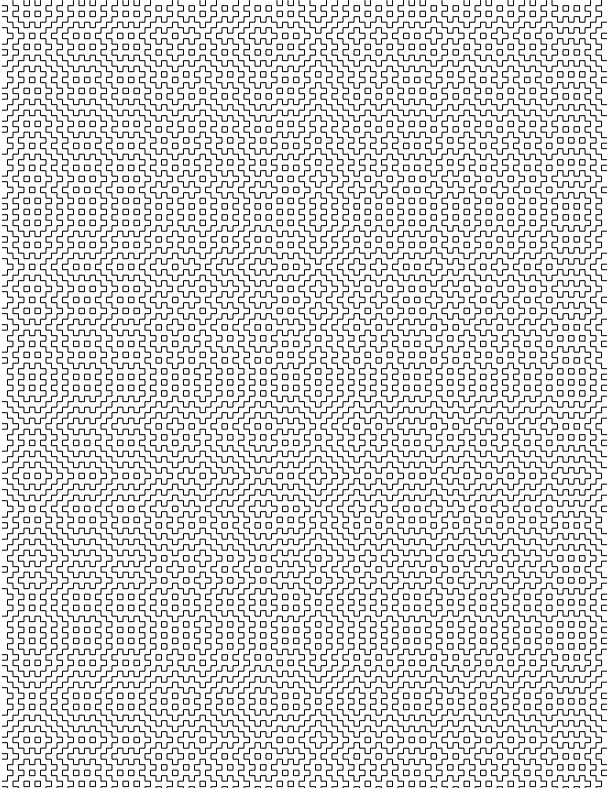
\includegraphics[width=\paperwidth,height=\paperheight]{random_rectangles.png}};
    \node[yshift=-50mm] at (current page.north west)
      {\begin{tikzpicture}[remember picture, overlay]
        \draw (0,0) (\paperwidth,3cm);
        \node[rounded corners = 5pt, anchor=west,xshift=.1\paperwidth,rectangle, inner sep=11pt, fill=black]
              {\makecell{\color{white}\chapterlabel \\ \color{white}#1}};
       \end{tikzpicture}
      };
   \end{tikzpicture}
 }
\titlespacing{\chapter}{0pt}{50pt}{-40pt}

\Opensolutionfile{ans}[allsolutions]

%%%%%%%%%%%%%%%%%%%%%%%%%%%%%%%%%%%%%%%%%%%%%%%%%%%%%%%%%%%%%%%%%%%%%%%%%%%%%%%%%%%%%%%%%%%%%%%%%%%%%%%%%%
%%%%%%%%%%%%%%%%%%%%%%%%%%%%%%%%%%%%%%%%%%%%%%%%%%%%%%%%%%%%%%%%%%%%%%%%%%%%%%%%%%%%%%%%%%%%%%%%%%%%%%%%%%
%%%%%%%%%%%%%%%%%%%%%%%%%%%%%%%%%%%%%%%%%%%%%%%%%%%%%%%%%%%%%%%%%%%%%%%%%%%%%%%%%%%%%%%%%%%%%%%%%%%%%%%%%%
%%%%%%%%%%%%%%%%%%%%%%%%%%%%%%%%%%%%%%%%%%%%%%%%%%%%%%%%%%%%%%%%%%%%%%%%%%%%%%%%%%%%%%%%%%%%%%%%%%%%%%%%%%
%%%%%%%%%%%%%%%%%%%%%%%%%%%%%%%%%%%%%%%%%%%%%%%%%%%%%%%%%%%%%%%%%%%%%%%%%%%%%%%%%%%%%%%%%%%%%%%%%%%%%%%%%%

\chapter{Logarithme népérien}
\newpage

\section{Calculs et équations}

\subsection{Calcul numérique \quad\small{(corrigé)}} 

\begin{enumerate}
	\item Exprimer chacun des nombres suivants en fonction de $\ln(2)$ :\\
	\renewcommand{\arraystretch}{1.5}
	\begin{tabular}{p{0.45\linewidth}p{0.45\linewidth}}
		$A=\ln(2)+\ln(4)+\ln(8)+\ln(16)$ & $B=\ln(48)-\ln(15)+\ln(20)$\\
		$C=\ln(1000)-\ln(400)-\ln(40)$ & $D=\ln(18)+\ln(28)-\ln(42)-\ln(24)$	\\
	\end{tabular}	
	
	\item Simplifier au maximum chacun des nombres suivants :\\
	\renewcommand{\arraystretch}{1.5}
	\begin{tabular}{p{0.45\linewidth}p{0.45\linewidth}}
		$A=\ln\left(\frac{1}{3}\right)-\ln\left(\frac{7}{5}\right)+\ln\left(\frac{3}{5}\right)+\ln\left(\frac{7}{9}\right)$ & $B=\ln\left((3+\sqrt{8})^{2024}\right)+\ln\left((3-\sqrt{8})^{2024}\right)$ \\
		$C=2\ln\left(1+\sqrt{2}\right)-\ln\left(3+2\sqrt{2}\right)$ & $D=2\ln\left(3e^2\right)+\ln\left(4e^3\right)-\ln(9e)$
	\end{tabular}
\end{enumerate}

\begin{hint}
	Utiliser les propriétés de la fonction logarithme népérien : $\ln(a)+\ln(b)=\ln(b)$ , $\ln(a)-\ln(b)=\ln\left(\frac{a}{b}\right)$ et $\ln\left(a^b\right)=b\ln(a)$
\end{hint}
\begin{sol}
\begin{enumerate}
	\item $A=10\ln(2) \quad B=6\ln(2) \quad C=-4\ln(2) \quad D=-\ln(2)$
	\item $A=-\ln(9) \quad B=0 \quad C=0 \quad D=6+2\ln(2)$ 
\end{enumerate}
\end{sol}



\subsection{Calcul littéral\quad\small{(corrigé)}}
Simplifier au maximum chacune des expressions suivantes sans prendre en compte leur domaine de validité :

\begin{tabular}{p{0.45\linewidth}p{0.45\linewidth}}
	$A=\ln(x)-\ln(1+x)+\ln(1+\frac{1}{x})$ & $B=\ln\left(\frac{x+1}{x-1}\right)-\ln\left(1+\frac{1}{x}\right)+\ln\left(\frac{x-1}{x}\right)$ \\
	$C=3\ln(x+1)-\ln\left(x^2+2x+1\right)$ & $D=\ln(x-1)+2\ln(x+1)-\ln(x^2-1)$
\end{tabular}

\,\,$E=\ln(x^2-1)-\ln(1+x^2)-\ln\left(1-\frac{1}{x^2}\right)+\ln\left(1+\frac{1}{x^2}\right)$

\,\,$F=\ln\left(\frac{1}{2}\right)+\ln\left(\frac{2}{3} \right)+\ln\left(\frac{3}{4}\right)+\ldots+\ln\left( \frac{n-1}{n}\right)$

\begin{sol}
	$A=0 \quad B=0 \quad C=\ln(x+1) \quad D=\ln(x+1) \quad E=0 \quad F=-\ln(n)$
\end{sol}



\subsection{Application à l'exponentielle}
Résoudre dans $\RR$ les équations suivantes :\\
\renewcommand{\arraystretch}{1.6}
\begin{tabular}{p{0.33\linewidth} p{0.33\linewidth} p{0.33\linewidth}}
a) $e^{2x-1} = 3$ & b) $2e^x + 2 = 4e^x-7$ & c) $e^{x^2} > 2$ \\
d) $3e^x - 2e^{3x} \leq 0$ & e) $e^{2x} + e^{2x+3} = 10$ & f) $2e^{2x-1} + e^{2x+1} = e^7$ \\
\end{tabular}



\subsection{Équations}
Résoudre dans $\RR$ les équations suivantes :\\
\renewcommand{\arraystretch}{1.6}
\begin{tabular}{p{0.35\linewidth} p{0.34\linewidth} p{0.32\linewidth}}
a) $\ln\left(2x+3\right) - \ln\left(5x\right) = 0$ & b) $\ln\left(x^2-4\right) - \ln\left(2-x\right) = 0$ & c) $\ln\left(x-\frac{1}{x}\right) + \ln\left(x\right) = 0$ \\
d) $2\ln\left(x+1\right) = -\ln(9)$ & e) $\ln\left(x\right) + \ln\left(x+1\right) = \ln\left(2x+2\right)$ &
f) $\ln\left(x^2 + 8x\right) - \ln\left(2x-9\right) = 0$ \\
g) $\ln\left(2x\right) - \ln\left(1-x^2\right) = \ln\left(3x-7\right)$ & h) $\ln\left(\frac{x}{2}\right) = \ln\left(4x\right) - \ln\left(1+e^x\right)$ & i) $\ln\left(2-e^x\right) = x$ \\
\end{tabular}




\subsection{Inéquations}
Résoudre dans $\RR$ les inéquations suivantes :\\
\renewcommand{\arraystretch}{1.6}
\begin{tabular}{p{0.34\linewidth} p{0.3\linewidth} p{0.33\linewidth}}
a) $\ln\left(x-1\right) - \ln\left(x\right) \leq 0$ & b) $\ln\left(e^{x}-1\right) > e$ & c) $e^{\ln\left(x\right)} \leq 2x-1$ \\
d) $\ln(x+2) - \ln(x+1) \geq \ln(x-1)$ & e) $\ln\left(x+e\right) - 2 > \ln\left(2x\right)$ & f) $\ln\left(x-1\right) + 1 < e$ \\
\end{tabular}



\subsection{Systèmes\quad\small{(corrigé)}}
Résoudre les systèmes suivants :

\renewcommand{\arraystretch}{2.5}
\begin{tabular}{p{0.29\textwidth} p{0.29\textwidth} p{0.35\textwidth}}
    $(S_1):\accol{e^xe^y=10\\e^{x-y}=\frac{2}{5}}$ & $(S_2):\accol{x-y=2\\\ln(x)+\ln(y)=3}$ & $(S_3):\accol{\ln(xy)=5+\ln(6)\\\ln(x+y)=2+\ln(3+2e)}$ \\
    $(S_4):\accol{\ln(x)+\ln(y)=5\\3\ln(x)+\ln(y)=3}$ & $(S_5):\accol{\ln(x)-\ln(y)=2\\\ln(x)=\ln\left(\frac{1}{y}\right)}$
\end{tabular}

\begin{sol}
\begin{tabular}{p{0.21\textwidth} p{0.38\textwidth} p{0.3\textwidth}}
	$S_1=\left\{\left(\ln(2);\ln(5)\right)\right\}$ & $S_2=\left\{\left(1+\sqrt{1+e^3};-1+\sqrt{1+e^3}\right)\right\}$ & $S_3=\left\{\left(3e^2;2e^3\right);\left(2e^3;3e^2\right)\right\}$\\
	$S_4=\left\{\left(\frac{1}{e};e^6\right)\right\}$ & $S_5=\left\{\left(e;\frac{1}{e}\right);\left(-e;\frac{-1}{e}\right)\right\}$
\end{tabular}
\end{sol}



\subsection{Équations logarithmiques\quad\small{(corrigé)}}
Résoudre dans $\RR$ les (in)équations suivantes en précisant leur domaine de validité :

\renewcommand{\arraystretch}{1.6}
\begin{tabular}{p{0.4\textwidth} p{0.4\textwidth}}
    a) $\ln(x)^2+\ln(x^2)=0$ & b) $\ln(x)^2+\ln(x)<2$ \\
    c) $\sqrt{\ln(x)}>\ln(x)$ & d) $\frac{\ln(x^3)}{\ln(x)^2}\geq-6$ \\
    e) $\ln(x)\ln(\frac{x}{e})\leq12$ & f) $\ln(x)^2+\ln(x^{1+e})+e=0$
\end{tabular}

\begin{hint}
	Utiliser le changement de variable $X=\ln(x)$
\end{hint}
\begin{sol}
	\begin{tabular}{p{0.4\textwidth} p{0.4\textwidth}}
		a) $S=\left\{1;e^{-2}\right\}$ & b) $S=\left]e^{-2};e\right[$ \\
		c) $S=]1;e[$ & d) $S=\left]0;e^{-\frac{1}{2}}\right]\cup]1;+\infty[$\\
		e) $S=\left[e^{-3};e^4\right]$ & f) $S=\left\{e^{-1};e^{-e}\right\}$
    \end{tabular}
\end{sol}



\subsection{Puissantes racines\quad\small{(corrigé)}}
Résoudre dans $\RR_+$ l'équation $x^{\sqrt{x}}=(\sqrt{x})^x$

\begin{hint}
	Résoudre l'équation en composant chaque membre par la fonction logarithme.
\end{hint}
\begin{sol}
	$S=\{0;1;4\}$
\end{sol}



\section{Application aux suites numériques}

\subsection{Inéquations géométriques}
Résoudre chacune des inéquations suivantes dans $\ZZ$ :\\
\begin{tabular}{p{0.3\linewidth} p{0.3\linewidth} p{0.3\linewidth}}
a) $1, 23^n \geq 123$ & b) $3 \times 2^n \geq 10^{21}$ & c) $\frac{1}{2 + 0,95^n} \geq 0,4999$ \\ 
d) $\frac{3 + \left(\frac{7}{9}\right)^{2n-1}}{5} \geq \frac{6 + 10^{-10}}{10}$ & e) $3^{n+17} \geq 2^{2n-1}$ & f) $0,7^{n-3} \geq 15 \times 0,8^n$ \\
\end{tabular}



\subsection{Suites géométriques}
\begin{enumerate}
    \item Soit $(u_n)$ géométrique de premier terme $u_0 = 4$ et de raison $q = \frac{5}{6}$

    À partir de quel rang $n$ a-t-on $u_n < \frac{1}{1000}$ ?

    \item Soit $(u_n)$ géométrique de premier terme $u_0 = \frac{1}{3}$ et de raison $q = \frac{24}{23}$

    À partir de quel rang $(u_n)$ dépasse-t-elle $123$ ?

    \item Soit $(u_n):\defsuite{u_0=-2}{\frac{3u_n}{2}}$. On pose $v_n = \frac{8}{1 - u_n}$

    À partir de quel rang a-t-on $v_n < \frac{3}{10}$ ?

    \item Soit $(u_n)$ géométrique de premier terme $u_0 = 5$ et de raison $q = 2$

    À partir de quel rang peut-on affirmer que $\frac{u_n}{12 + u_n} > \frac{100}{101}$ ?
\end{enumerate}



\subsection{Suite très exponentielle\quad\small{(corrigé)}}
On définit la suite $\Un$ par $\defsuite{u_0=-1}{2u_n-3u_n\,^2}$ et on admet que la suite $\Un$ est négative. \\
Pour tout $\nN$ on pose $v_n=\ln(1-3u_n)$
\begin{enumerate}
	\item Montrer que la suite $(v_n)$ est géométrique de raison 2.
	\item En déduire l'expression de $u_n$ en fonction de $n$.
\end{enumerate}

\begin{hint}
	\begin{enumerate}
		\item Exprimer $v_{n+1}$ en fonction de $v_n$ et repérer une identité remarquable.
		\item Exprimer $v_n$ en fonction de $n$ puis $u_n$ en fonction de $v_n$
	\end{enumerate}
\end{hint}
\begin{sol}
	2. $u_n=\frac{1-2^{2^{n+1}}}{3}$
\end{sol}



\subsection{Seuil et somme}
Soit $(u_n)$ une suite géométrique telle que $u_5=\frac{1}{9}$ et $u_7=4$\\
À partir de quel rang pourra-t-on affirmer que $\sommek{0}{n}u_k \geq 1000$ ?


\section{Étude de fonctions}

\subsection{Échange d'exposant\quad\small{(corrigé)}}
On cherche à déterminer les entiers naturels $n$ tels que $n^3\geq3^n$
\begin{enumerate}
    \item Montrer que résoudre le problème revient à résoudre l'inéquation $3\ln(n)-n\ln(3)\geq0$
    \item On pose $f(x)=3\ln(x)-x\ln(3)$
    \begin{enumerate}
        \item Dresser le tableau de variations de la fonction $f$
        \item En déduire que $f$ est négative sur $[3;+\infty[$
    \end{enumerate}
    \item Calculer $n^3$ et $3^n$ pour $n\in\{0;1;2\}$
    \item En déduire alors que $n=3$ est l'unique solution au problème
    \item [$\dur$] Comparer les nombres $e^{\pi}$ et $\pi^e$
\end{enumerate}

\begin{hint}
	\begin{enumerate}
		\item Appliquer la fonction logarithme sur chaque membre de l'inégalité.
		\item Utiliser $\left(\ln(x)\right)'=\frac{1}{x}$ et penser à calculer $f(3)$
		\item[4.] Utiliser les questions précédentes.
	\end{enumerate}
\end{hint}
\begin{sol}
	\begin{enumerate}
		\item[2.] La valeur de $f\left(\frac{3}{\ln(3)}\right)$ est approchée à $10^{-3}$\\
		\begin{tikzpicture}
			\tkzTabInit[espcl=5pt]{$x$/1,$f'(x)$/1,$f(x)$/2}{$0$,$\frac{\ln(3)}{3}$,$+\infty$}
			\tkzTabLine {d , + , z , -}				
			\tkzTabVar {D-/, +/{$0,015$} , -/}
            \tkzTabVal{2}{3}{0.5}{$3$}{$0$}
		\end{tikzpicture} 
	\end{enumerate}
\end{sol}



\subsection{Drôle de définition\quad\small{(corrigé)}}
On pose $g(x)=\sqrt{\ln(x-x^2)}$.

Déterminer $\Dcal_g$ le domaine de définition de la fonction $g$.

\begin{hint}
	Il s'agit d'une fonction composée, commencer par déterminer sous quelles conditions le logarithme peut exister, puis s'intéresser à la racine carrée.
\end{hint}
\begin{sol}
	$\Dcal_g=\emptyset$
\end{sol}



\subsection{Encadrement\quad\small{(corrigé)}}
\begin{enumerate}
    \item Montrer que $\ln(1+x)\leq x$ pour tout $x>-1$
    \item Montrer que $x-\frac{x^2}{2}\leq \ln(1+x)$ pour tout $x\geq0$
\end{enumerate}

\begin{hint}
	\begin{enumerate}
		\item Dresser le tableau de variations de la fonction $f:x\mapsto x-\ln(1+x)$ sur $]1;+\infty[$
		\item Dresser le tableau de variations de la fonction $g:x\mapsto x-\frac{x^2}{2}-\ln(1+x)$ sur $[0;+\infty[$
	\end{enumerate}
\end{hint}
\begin{sol}
	\begin{enumerate}
		\item $f'(x)=\frac{x}{1+x}$, on a donc le tableau suivant :\\
		\begin{tikzpicture}
			\tkzTabInit[espcl=5pt]{$x$/1 , $f'(x)$/1 , $f(x)$/2}{$-1$ , $0$ , $+\infty$}
			\tkzTabLine {d , - , z , +}
			\tkzTabVar {D+/ , -/$0$ , +/}
		\end{tikzpicture}
		
		On voit que $f(x)\geq0$ sur $]1;+\infty[$, ce qui conclut notre preuve.
		\item $g'(x)=\frac{x^2}{1+x}$, on a donc le tableau suivant :\\
		\begin{tikzpicture}
			\tkzTabInit[espcl=5pt]{$x$/1 , $g'(x)$/1 , $g(x)$/2}{$0$ , $+\infty$}
			\tkzTabLine { , - , }
			\tkzTabVar {+/0 , -/}
		\end{tikzpicture}
		
		On voit que $g(x)\leq0$ sur $[0;+\infty[$, ce qui conclut notre preuve.
	\end{enumerate}
\end{sol}



\subsection{Variations annexes}
On pose $f(x) = x - \frac{\ln(x)}{x}$ et $g(x)=x^2+\ln(x)-1$
\begin{enumerate}
    \item Dresser le tableau de variations de $g$ en faisant figurer de la valeur de $g(1)$
    \item Exprimer $f'(x)$ en fonction de $g(x)$
    \item Dresser le tableau de variations de $f$
    \item Déterminer l'équation réduite de $T$, la tangente à $C_f$ au point d'abscisse $e$
\end{enumerate}



\subsection{Logarithme et exponentielle}
On pose $h(x) = x+e^{-x}$ et $\ell(x) = \ln(h(x))$

\begin{enumerate}
    \item Dresser le tableau de variations de $h$
    \item Justifier que $\ell$ est définie sur $\mathbb{R}$
    \item Dresser le tableau de variations de $\ell$
    \item Déterminer l'équation réduite de $T$ la tangente à $C_f$ au point d'abscisse $1$
\end{enumerate}


\subsection{Joli quotient}
On pose $\varphi(x) = \ln(x + x^2) + \frac{x + 7}{x + 1}$
\begin{enumerate}
    \item Déterminer $\mathcal{D}$ le domaine de définition de $\varphi$
    \item Montrer que pour tout $x \in \mathcal{D}$, $\varphi'(x) = \frac{2x^2 - 3x + 1}{x(x + 1)^2}$
    \item Dresser le tableau de variations de $\varphi$
\end{enumerate}



\subsection{Produit de référence\quad\small{(corrigé)}}
Étudier les variations de $f:x\mapsto\ln(x)e^x$ sur son domaine de définition

\begin{hint}
On pourra étudier les variations de la fonction $x:\mapsto\ln(x)+\frac{1}{x}$
\end{hint}
\begin{sol}
	$\Dcal_f=\RR_+^*$ et on a $f'(x)=e^x\left(\frac{1}{x}+\ln(x)\right)=e^xg(x)$
	
	Or $g'(x)=\frac{x-1}{x^2}$, on obtient donc le tableau suivant :\\
	\begin{tikzpicture}
		\tkzTabInit[espcl=5pt]{$x$/1 , $g'(x)$/1 , $g(x)$/2}{$0$ , $1$ , $+\infty$}
		\tkzTabLine {d , - , z , +}
		\tkzTabVar {D+/ , -/$1$ , +/}
	\end{tikzpicture}
	
	On voit que la fonction $g$ est strictement positive sur $\RR_+^*$, ce qui implique que $f'$ est strictement positive sur $\RR_+^*$, ainsi $f$ est strictement croissante sur son domaine de définition.
\end{sol}



\subsection{Tangentes\quad\small{(corrigé)}}
\begin{enumerate}
    \item Existe-t-il un point de la courbe représentative de la fonction logarithme pour lequel la tangente à cette courbe passe par le point de coordonnées $(0;1)$ ?
    \item Soit $f:x\mapsto\frac{\ln(x)}{x}$\\
    Existe-t-il un point de $\Ccal_f$ auquel la tangente à $\Ccal_f$ passe par l'origine du repère ?
\end{enumerate}

\begin{hint}
	\begin{enumerate}
		\item Déterminer l'équation réduite de la tangente à la courbe du logarithme en un point d'abscisse $a>0$, puis injecter les coordonnées du point $(0;1)$
		\item Déterminer l'équation réduite de la tangente à $\Ccal_f$ en un point d'abscisse $a>0$ puis injecter les cordonnées de l'origine du repère/
	\end{enumerate}
\end{hint}
\begin{sol}
	\begin{enumerate}
		\item Au point $A\left(e^2;2\right)$, la tangente à la courbe du logarithme est $T:y=\frac{x}{e^2}+1$ et passe bien par le point de coordonnées $(0;1)$
		\item Au point $B\left(e^{\frac{1}{2}};\frac{e^{-\frac{1}{2}}}{2}\right)$, la tangente à $\Ccal_f$ est $T:y=\frac{x}{2e}$ et passe bien par l'origine du repère.
	\end{enumerate}
\end{sol}



\subsection{Étude d'une fonction\quad\small{(corrigé)}}
On considère la fonction $f$ définie sur $\RR_+^*\setminus\{1\}$ par $f(x)=\frac{x}{\ln(x)}$
\begin{enumerate}
    \item Montrer que $f'(x)=\frac{1}{\ln(x)}-\frac{1}{\ln(x)^2}$
    \item Dresser le tableau de variations de $f$
    \item Montrer qu'aucune tangente à $\Ccal_f$ ne peut avoir un coefficient directeur égal à 2.
    \item Déterminer les tangentes à $\Ccal_f$ ayant un coefficient directeur égal à -2.
\end{enumerate}

\begin{hint}
	\begin{enumerate}
		\item[3.] Rappeler que le coefficient directeur de la tangente à $\Ccal_f$ est donné par $f'(x)$ puis utiliser le changement de variable $X=\ln(x)$
		\item[4.] Rappeler que le coefficient directeur de la tangente à $\Ccal_f$ est donné par $f'(x)$ puis utiliser le changement de variable $X=\ln(x)$
	\end{enumerate}
\end{hint}
\begin{sol}
	\begin{enumerate}
		\item[2.] $f'(x)=\frac{\ln(x)-1}{\ln(x)^2}$, on a donc le tableau suivant :\\
		\begin{tikzpicture}
			\tkzTabInit[espcl=5pt] {$x$ /1 , $f'(x)$ /1 , $f(x)$/2}{$0$ , $1$ , $e$ , $+\infty$}
			\tkzTabLine {d , - , d , - , z , +}
			\tkzTabVar {D+/ , D+/ , -/$e$ ,+/} 
		\end{tikzpicture}
		\item[3.] On cherche à résoudre l'équation $f'(x)=2$, ce qui équivaut à $2\ln^2(x)-\ln(x)+1=0$\\
		On pose alors $X=\ln(x)$ et on voit que cette équation n'a pas de solution.
		\item[4.] On cherche à résoudre l'équation $f'(x)=-2$, ce qui équivaut à $2\ln^2(x)+\ln(x)-1=0$\\
		On pose alors $X=\ln(x)$, et on obtient après résolution de l'équation $x=\sqrt{e}$ ou $x=\frac{1}{e}$\\
		On donne alors l'équation des tangentes à $\Ccal_f$ aux points d'abscisse trouvées : $T_1:y=-2x+\frac{1}{e}$ et $T_2:y=-2x+4\sqrt{e}$
	\end{enumerate}
\end{sol}



\subsection{On élève le degré\quad\small{(corrigé)}}
On définit la fonction $h$ sur $[-1;+\infty[$ par $h(x)=x-\ln\left(2+x^3\right)$
\begin{enumerate}
	\item Déterminer l'expression de $h'(x)$ en fonction de $x$
	\item Déterminer un polynôme du second degré $P$ pour lequel $h'(x)=\frac{(x-1)P(x)}{2+x^3}$
	\item Dresser le tableau de variations de $h$ en donnant une valeur approchée à $10^{-3}$ de ses extremums.
\end{enumerate}

\begin{hint}
	\begin{enumerate}
	\item[2.] Écrire $P(x)=ax^2+bx+c$ puis déterminer les valeurs de $a$, $b$ et $c$ pour que les expressions soient égales.
	\end{enumerate}
\end{hint}
\begin{sol}
	\begin{enumerate}
		\item $h'(x)=1-\frac{3x^2}{2+x^3}$
		\item $P(x)=x^2-2x-2$
		\item \begin{tikzpicture}
			\tkzTabInit {$x$/1 , $h'(x)$/1 , $h(x)$/2} {$-1$ , $1-\sqrt{3}$ , $1$ , $1+\sqrt{3}$ , $+\infty$}
			\tkzTabLine {, - , z , + , z , - , z , + , }
			\tkzTabVar {+/{$-1$} , -/{$-1,207$} , +/{$-0,099$} , -/{$-0,377$} , +/}
		\end{tikzpicture}
	\end{enumerate}
\end{sol}



\subsection{Sans faire de vagues\quad\small{(corrigé)}}
Soit $\phi:x\mapsto\frac{\ln\left(1+x^2\right)}{1+x^2}$ définie sur $\RR$
\begin{enumerate}
	\item Montrer que $\phi'(x)=-2x\frac{\ln\left(1+x^2\right)-1}{\left(1+x^2\right)^2}$
	\item Justifier que $\phi'$ s'annule en $0$, en $\sqrt{e-1}$ et en $-\sqrt{e-1}$
	\item Dresser le tableau de variations de la fonction $\phi$
\end{enumerate}

\begin{sol}
	\begin{tikzpicture}
		\tkzTabInit {$x$/1 , $\phi'(x)$/1 , $\phi(x)$/2} {$-\infty$ , $-\sqrt{e-1}$ , 0 , $\sqrt{e-1}$ , $+\infty$}
		\tkzTabLine { , + , z , - , z , + , z}
		\tkzTabVar {-/ , +/{$\frac{1}{e}$} , -/0 , +/{$\frac{1}{e}$} , -/}
	\end{tikzpicture}
	\vspace{10pt}
\end{sol}



\subsection{Logarithme et somme\quad\small{(corrigé)}}
\begin{enumerate}
	\item Dresser le tableau de variations de la fonction $f:x\mapsto \ln(x)-x+1$ définie sur $\RR_+^*$
	\item Dresser le tableau de variations de la fonction $g:x\mapsto \frac{x-1}{x}-\ln(x)$ définie sur $\RR_+^*$
    \item Montrer que $\frac{x-1}{x}\leq\ln(x)\leq x-1$ pour tout $x\in\RR^*_+$ 
    \item À l'aide d'un changement de variable, en déduire que pour $x\in\RR^*_+$ on a $\frac{1}{x+1}\leq\ln\left(\frac{1+x}{x}\right)\leq\frac{1}{x}$
    \item Calculer la somme $\ln\left(\frac{2}{1}\right)+\ln\left(\frac{3}{2}\right)+\ln\left(\frac{4}{3}\right)+\ldots+\ln\left(\frac{1+n}{n}\right)$ pour $\nN^*$
    \item En utilisant l'inégalité de la question 4. montrer que $\frac{1}{2}+\frac{1}{3}+\frac{1}{4}+\ldots+\frac{1}{n+1}\leq\ln\left(1+n\right)$
\end{enumerate}

\begin{hint}
	\begin{enumerate}
		\item[3.] Utiliser le signe des fonctions $f$ et $g$
		\item[4.] Poser $X=\frac{1+x}{x}$
		\item[5.] Utiliser les propriétés de la fonction logarithme.
	\end{enumerate}
\end{hint}
\begin{sol}
	\begin{enumerate}
	\begin{minipage}{0.45\linewidth}
	\item \begin{tikzpicture}
			\tkzTabInit[espcl=2.5pt] {$x$/1 , $f'(x)$/1 , $f(x)$/2} {$0$ , $1$ , $+\infty$}
			\tkzTabLine {d , + , z , -}
			\tkzTabVar {D-/ , +/$0$ , -/}
		\end{tikzpicture}
	\end{minipage}\hfill
	\begin{minipage}{0.45\linewidth}
	\item \begin{tikzpicture}
			\tkzTabInit[espcl=2.5pt] {$x$/1 , $g'(x)$/1 , $g(x)$/2} {$0$ , $1$ , $+\infty$}
			\tkzTabLine {d , + , z , -}
			\tkzTabVar {D-/ , +/$0$ , -/}
		\end{tikzpicture}
	\end{minipage}
	\item $f(x)\leq0$ donc $\ln(x)\leq x-1$ sur $\RR^*_+$\\
	$g(x)\leq0$ donc $\ln(x)\geq \frac{x-1}{x}$ sur $\RR^*_+$\\
	On a bien les deux inégalités demandées.
	\item Pour $\xR^*_+$ on pose $X=\frac{1+x}{x}$. Alors $X\in\RR^*_+$. Donc d'après la question 3. on a :\\
	$\frac{X-1}{X}\leq\ln(X)\leq X-1$.\\
	En remplaçant dans ces inégalités $X$ par $\frac{1+x}{x}$ et en simplifiant, on obtient bien $\frac{1}{x+1}\leq\ln\left(\frac{1+x}{x}\right)\leq\frac{1}{x}$
	\item $\ln\left(\frac{2}{1}\right)+\ln\left(\frac{3}{2}\right)+\ln\left(\frac{4}{3}\right)+\ldots+\ln\left(\frac{1+n}{n}\right) = \ln(1+n)$
	\item D'après la question 4. pour tout $k\in\NN$ on peut affirmer que $\frac{1}{k+1}\leq\ln\left(\frac{1+k}{k}\right)$, ainsi :\\
	$\frac{1}{2}+\frac{1}{3}+\frac{1}{4}+\ldots+\frac{1}{n+1}\leq\ln\left(\frac{2}{1}\right)+\ln\left(\frac{3}{2}\right)+\ln\left(\frac{4}{3}\right)+\ldots+\ln\left(\frac{1+n}{n}\right)=\ln(1+n)$
	\end{enumerate}
\end{sol}



\subsection{Aire d'un rectangle\quad\small{(corrigé)}}
On définit sur $\RR+^*$ les fonctions $f$ et $g$ par : $f(x)=\frac{\ln(x)}{x}+\frac{2}{x^2}-\frac{1}{x}$ et $g(x)=x\ln(x)+2-x$.\\
On note $\Ccal_f$ la courbe représentative de la fonction $f$ dans un repère orthonormé $\Oij$.

\begin{minipage}{0.52\linewidth}
\begin{enumerate}
	\item Dresser le tableau de variations de la fonction $g$
	\item En déduire que $f$ est positive sur $\RR_+^*$
	\item On considère $M$ un point de $\Ccal_f$ d'abscisse $a$, ainsi que $P$ et $Q$ ses projetés orthogonaux sur les axes du repère comme représenté ci-contre :
	\begin{enumerate}
		\item Exprimer l'aire du rectangle $MPOQ$ en fonction de $a$.
		\item Déterminer l'aire minimale que peut avoir le rectangle $MPOQ$, et préciser alors la position du point $M$.
	\end{enumerate}
\end{enumerate}
\end{minipage}\hfill
\begin{minipage}{0.45\linewidth}
	\begin{tikzpicture} % ----- Début de la figure

    \begin{axis}[xmin = 0, xmax = 3, ymin = 0, ymax = 3, xtick distance=1, ytick distance=1, grid = major,
        %minor grid style = {line width = 0.1pt , draw = gray!20},
        major grid style = {line width = 0.2pt , draw = gray},
        axis lines = middle, minor tick num = 5, enlargelimits = { abs = 0.2 }, 
        ticklabel style = {font = \tiny }
        ]

    \addplot[line width = 2pt , domain=0.1:5, samples=100, color=red]   
    {ln(x)/x+2/(x^2)-1/x};
    
    \draw[color=blue , dashed , line width = 1.5pt] (0.8,1.6)--(0.8,0);
    \draw[color=blue , dashed , line width = 1.5pt] (0.8,1.6)--(0,1.6);
    \node[right] at (0.8,1.6) {$M$}; \node[left] at (0,1.6) {$P$}; \node at (1,0.15) {$Q$};
    \node at (-0.1,0.15) {$O$};
    \path[pattern color=blue,pattern=stripe,stripe angle=25,stripe size=15pt] (0,0)--(0.8,0)--(0.8,1.6)--(0,1.6)--(0,0);
    \node[color=red] at (2.2,0.5) {$\Ccal_f$};
    \end{axis}
\end{tikzpicture}
\end{minipage}

\begin{hint}
	\begin{enumerate}
		\item[2.] Exprimer $f(x)$ en fonction de $g(x)$
	\end{enumerate}
\end{hint}
\begin{sol}
	\begin{enumerate}
		\item \begin{tikzpicture}
			\tkzTabInit[espcl=5pt] {$x$/1 , $g'(x)$/1 , $g(x)$/2} {$0$ , $1$ , $+\infty$}
			\tkzTabLine {d , - , z , + , }
			\tkzTabVar {D+/ , -/1 , +/}
		\end{tikzpicture}
		\item $g$ est positive sur $\RR^*_+$ et $f(x)=\frac{g(x)}{x^2}$ donc $f$ est positive sur $\RR^*_+$
		\item \begin{enumerate}
			\item $\Acal_{MPOQ}=af(a)$
			\item En posant $\Acal(a)=af(a)$, on obtient $\Acal'(a)=\frac{a-2}{a^2}$\\
			On peut alors dresser le tableau de variations de $\Acal$ et on voit que son minimum est atteint en $a=2$, Or $\Acal(2)=\ln(2)$
		\end{enumerate}		 
	\end{enumerate}
\end{sol}



%%%%%%%%%%%%%%%%%%%%%%%%%%%%%%%%%%%%%%%%%%%%%%%%%%%%%%%%%%%%%%%%%%%%%%%%%%%%%%%%%%%%%%%%%%%%%%%%%%%%%%%%%%
%%%%%%%%%%%%%%%%%%%%%%%%%%%%%%%%%%%%%%%%%%%%%%%%%%%%%%%%%%%%%%%%%%%%%%%%%%%%%%%%%%%%%%%%%%%%%%%%%%%%%%%%%%
%%%%%%%%%%%%%%%%%%%%%%%%%%%%%%%%%%%%%%%%%%%%%%%%%%%%%%%%%%%%%%%%%%%%%%%%%%%%%%%%%%%%%%%%%%%%%%%%%%%%%%%%%%
%%%%%%%%%%%%%%%%%%%%%%%%%%%%%%%%%%%%%%%%%%%%%%%%%%%%%%%%%%%%%%%%%%%%%%%%%%%%%%%%%%%%%%%%%%%%%%%%%%%%%%%%%%
%%%%%%%%%%%%%%%%%%%%%%%%%%%%%%%%%%%%%%%%%%%%%%%%%%%%%%%%%%%%%%%%%%%%%%%%%%%%%%%%%%%%%%%%%%%%%%%%%%%%%%%%%%


\chapter{Convexité}
\newpage


\section{Dérivation et convexité}

\subsection{Dérivée\quad\small{(corrigé)}}
Déterminer la dérivée de chacune des fonctions suivantes sans tenir compte de leur domaine de définition :

\begin{tabular}{p{0.3\linewidth}p{0.3\linewidth}p{0.3\linewidth}}
$f_1:x\mapsto\sqrt{1+x^2+x^3}$ & $f_2:x\mapsto e^{x+\frac{1}{x}}$ & $f_3:x\mapsto (2x-e^x)^7$\\
$f_4:x\mapsto \ln\left(x^2-3\sqrt{x}\right)$ & $f_5:x\mapsto\left(6-\ln(x)\right)^4$ & $f_6:x\mapsto xe^{x^2}$\\
$f_7:x\mapsto e^{x\ln(x)}-7x$ & $f_8:x\mapsto (x^2-1)e^{3+2x}$ & $f_9:x\mapsto(2x+3)\sqrt{1+x^2}$ \\
$f_{10}:x\mapsto \frac{2-6x}{e^{1+x^2}}$ & $f_{11}:x\mapsto \frac{x^2-x-1}{\sqrt{5x+2}}$ & $f_{12}:x\mapsto\frac{xe^x}{\sqrt{3+2x}}$\\
$f_{13}(x)= \left(1+e^{x^2+1}\right)^{4}$ & $f_{14}:x\mapsto \sqrt{\ln(x-x^2)}$ & $f_{15}:x\mapsto e^{\sqrt{1+\ln(x)}}$
\end{tabular}

\begin{sol}
\renewcommand{\arraystretch}{2}
	\begin{tabular}{p{0.3\linewidth}p{0.3\linewidth}p{0.3\linewidth}}
	$f_1'(x)=\frac{2x+3x^2}{\sqrt{1+x^2+x^3}}$ & $f_2'(x)=\left(1-\frac{1}{x^2}\right)e^{x+\frac{1}{x}}$ & $f_3'(x)=\left(14-7e^x\right)(2x-e^x)^6$ \\
	$f_4'(x)=\frac{3-4x\sqrt{x}}{6x-2x^2\sqrt{x}}$ & $f_5'(x)=-\frac{4\left(6-\ln(x)\right)^3}{x}$ & $f_6'(x)=\left(2x^2+1\right)e^{x^2}$ \\
	$f_7'(x)=e^{x\ln(x)}(1+\ln(x))-7$ & $f_8'(x)=(2x^2+2x-2)e^{3+2x}$ & $f_9'(x)=\frac{4x^2+3x+2}{\sqrt{1+x^2}}$ \\	
	$f_{10}'(x)=\frac{12x^2-4x-6}{x^{x^2+1}}$ & $f_{11}'(x)=\frac{15x^2+3x+1}{(10x+4)\sqrt{5x+2}}$ & $f_{12}'(x)=\frac{(2x^2+4x+3)e^x}{(2x+3)\sqrt{2x+3}}$ \\
	$f_{13}'(x)=8xe^{1+x^2}\left(1+e^{1+x^2}\right)^{3}$ & $f_{14}'(x)=\frac{2x-1}{x(2x-2)\sqrt{\ln(x-x^2}}$ & $f_{15}'(x)=\frac{e^{\sqrt{1+\ln(x)}}}{2x\sqrt{1+\ln(x)}}$
\end{tabular}
\end{sol}



\subsection{Variations\quad\small{(corrigé)}}
Dresser le tableau de variation des fonctions suivantes en précisant leur domaine de définition :

$f:x\mapsto\frac{\sqrt{1+x^2}}{1+x}$ \qquad $g:x\mapsto e^{1-2x}\sqrt{x}$ \qquad $h:x\mapsto x\left(1-\sqrt{x}\right)^5$ \qquad $\rho:x\mapsto x\sqrt{2x+x^2}$ 

\begin{sol}
\begin{minipage}{0.45\linewidth}
	\begin{tikzpicture}
		\tkzTabInit[espcl=1.75]{$x$ /1, $f(x)$ /2}{$-\infty$ , $-1$ , $1$ , $+\infty$}
		\tkzTabVar{+/, -D+/ , -/$\frac{\sqrt{2}}{2}$,+/}
	\end{tikzpicture}
	
	\begin{tikzpicture}
		\tkzTabInit{$x$ /1, $h(x)$ /2}{$0$ , $\frac{4}{49}$ , $+\infty$}
		\tkzTabVar{-/$0$ , +/$\frac{4\times5^5}{7^7}$, -/}
	\end{tikzpicture}
\end{minipage}\hfill
\begin{minipage}{0.45\linewidth}
	\begin{tikzpicture}
		\tkzTabInit{$x$ /1, $g(x)$ /2}{$0$,$\frac{1}{4}$,$+\infty$}
		\tkzTabVar{-/$0$ , +/$\frac{1}{2}e^{\frac{1}{2}}$, -/}
	\end{tikzpicture}
	
	\begin{tikzpicture}
		\tikzset{h style/.style = {pattern=north west lines}}
		\tkzTabInit[espcl=1.75]{$x$ /1, $\rho(x)$ /2}{$-\infty$,$-2$,$0$,$+\infty$}
		\tkzTabVar{-/ , +H/$0$ / , -/$0$ / , +/ }
	\end{tikzpicture}
\end{minipage}
\vspace{10pt}
\end{sol}



\subsection{Dérivée seconde\quad\small{(corrigé)}}
Dériver deux fois les fonctions suivantes en précisant leur domaine de définition :

\begin{tabular}{p{0.25\linewidth}p{0.2\linewidth}p{0.2\linewidth}p{0.25\linewidth}}
$f_1(x)=x^5-2x^4+x^2-1$ & $f_2(x)=x^2e^x$ & $f_3(x)=\frac{x^2+1}{x}$ & $f_4(x)=(x+1)\sqrt{x}$\\
$f_5(x)=xe^{x^2}$ & $f_6(x)=\sqrt{1-x^2}$ & $f_7(x)=e^{\sqrt{x}}$ & $f_8(x)=\frac{4x\sqrt{x}}{e^x}$
\end{tabular}

\begin{sol}
	\begin{tabular}{p{0.23\linewidth}p{0.23\linewidth}p{0.18\linewidth}p{0.25\linewidth}}
		$f_1''(x)=20x^3-24x^2+2$ & $f_2''(x)=(x^2+4x+2)e^x$ & $f_3''(x)=\frac{2}{x^3}$ & $f_4''(x)=\frac{3x-1}{4x\sqrt{x}}$\\
		$f_5''(x)=2x(2x^3+3)e^{x^2}$ & $f_6''(x)=\frac{-1}{(1-x^2)\sqrt{1-x^2}}$ & $f_7''(x)=\frac{e^{\sqrt{x}}(\sqrt{x}-1)}{4x\sqrt{x}}$ & $f_8''(x)=\frac{4x^2-12x+3}{\sqrt{x}e^x}$
	\end{tabular}
\end{sol}



\subsection{Exponentielle à paramètres\quad\small{(corrigé)}}
Soient $a$ et $b$ deux nombres réels quelconques.

Montrer que la fonction $f$ définie par $f(x)=e^{ax+b}$ est convexe sur $\RR$

\begin{sol}
	$f''(x)=a^2e^{ax+b} > 0$, donc $f$ est convexe.\\
\end{sol}



\subsection{Sur la fonction exponentielle\quad\small{(corrigé)}}
Soit $g(x)=e^x$ pour tout $\xR$\\
On considère $A$ et $B$ les points de $\Ccal_g$ d'abscisses respectives 0 et 1
\begin{enumerate}
	\item Justifier que $g$ est convexe sur $\RR$
    \item Étudier la position relative de $\Ccal_g$ et de $(AB)$
    \item Déterminer l'équation réduite de la droite $(AB)$
    \item Résoudre sur $\RR$ l'équation $e^x+x\geq1+ex$
\end{enumerate}

\begin{hint}
	\begin{enumerate}
		\item Utiliser une définition de la convexité.
		\item Utiliser le fait que $[AB]$ est une corde de $\Ccal_g$
		\item[4.] Reprendre les questions précédentes
	\end{enumerate}
\end{hint}
\begin{sol}
	\begin{enumerate}
		\item $g'(x)=e^x$ donc $g'$ est croissante, donc $g$ est convexe.
		\item $\Ccal_g$ est en-dessous de $(AB)$ sur $[0;1]$, et au-dessus sinon.
		\item $(AB):y=(e-1)x+1$
		\item $e^x+x\geq1+ex \Leftrightarrow e^x\geq(e-1)x+1$ donc $S=]-\infty;0]\cup[1;+\infty[$
	\end{enumerate}
\end{sol}



\subsection{Moyenne et convexité\quad\small{(corrigé)}}
On considère la fonction $f:x\mapsto x^2$ définie sur $\RR$ ainsi que deux nombres réels quelconques $a$ et $b$. \\
On note $A$, $B$ et $J$ les points de $\Ccal_f$ d'abscisses respectives $a$, $b$ et $\frac{a+b}{2}$\\
On admettra que la fonction $f$ est convexe sur $\RR$
\begin{enumerate}
    \item Représenter la situation sur un graphique
    \item Calculer l'ordonnée des points $A$, $B$ et $J$
    \item On note $K$ le milieu du segment $[AB]$\\
    Calculer les coordonnées du point $K$
    \item Que peut-on dire concernant les points $J$ et $K$ ?
    \item En déduire que $(a+b)^2\leq2(a^2+b^2)$ puis que $a^2+b^2\geq2ab$
\end{enumerate}

\begin{hint}
	\begin{enumerate}
		\item[3.] Utiliser la formule des coordonnées du milieu d'un segment.
		\item[4.] Comparer leurs ordonnées grâce à la convexité de $f$
		\item[5.] reprendre les deux questions précédentes.
	\end{enumerate}
\end{hint}
\begin{sol}
	\begin{enumerate}
	\begin{minipage}{0.5\linewidth}
		\item \begin{tikzpicture}
    		\begin{axis}[xmin = -3, xmax = 6, ymin = 0, ymax = 37,
    		xtick distance=1, ytick distance=5, grid = major,
       		major grid style = {line width = 0.2pt , draw = gray},
        	axis lines = middle, enlargelimits = { abs = 0.2 }, 
        	ticklabel style = {font = \tiny }]
    			\addplot[line width = 2pt , domain=-3:6, samples=100, color=red]   
    			{x^2};
    			\node[color=red] at (2.2,0.5) {$\Ccal_f$};
    			\draw[color=blue,line width=1pt] (-2,4)--(4,16);
    			\draw[color=blue] node[above] at (-2,4) {$A$};
    			\draw[color=blue] node at (-2,4) {x};
    			\draw[color=blue] node[above] at (4,16) {$B$};
    			\draw[color=blue] node at (4,16) {x};
    			\draw[color=blue] node[above] at (1,1) {$J$};
    			\draw[color=blue] node at (1,1) {x};
    			\draw[color=blue] node[above] at (1,10) {$K$};
    			\draw[color=blue] node at (1,10) {x};
    		\end{axis}
    	\end{tikzpicture}
    	\end{minipage}
    	\begin{minipage}{0.5\linewidth}
    	\item $y_A=a^2 \quad y_B=b^2 \quad y_J=\frac{(a+b)^2}{4}$\\
    	\item $x_K=\frac{a+b}{b} \quad y_K=\frac{a^2+b^2}{2}$\\
    	\item La fonction $f$ est convexe, $J$ et $K$ ont la même abscisse mais $K$ se situe sur une corde de $\Ccal_f$ alors que $J$ se situe sur $\Ccal_f$. On en déduit donc que l'ordonnée de $K$ est supérieure à celle de $J$\\
    	\item En reprenant les questions 3. et 4. on obtient $\frac{a^2+b^2}{2}\geq\frac{(a+b)^2}{4}$ donc $(a+b)^2\leq2(a^2+b^2)$\\
    	En développant l'identité remarquable ci-dessus on obtient rapidement que $a^2+b^2\geq2ab$
    	\end{minipage}
	\end{enumerate}
\end{sol}



\subsection{Vrai / Faux\quad\small{(corrigé)}}
\begin{center}
\renewcommand{\arraystretch}{1.5}
\begin{tabular}{|p{4mm}|p{0.55\textwidth}|p{0.1\textwidth}|p{0.1\textwidth}|} \hline
    \no & \centering Proposition & Vrai & Faux \\ \hline
    1. & La somme de deux fonctions concaves est concave & & \\ \hline
    2. & Si $u$ est une fonction convexe, alors $e^u$ est également convexe & & \\ \hline
    3. & Si $u$ est une fonction positive et convexe, alors $\sqrt{u}$ est également convexe & & \\ \hline
    4. & Si $u$ est une fonction concave, alors $u^2$ est convexe & & \\ \hline
    5. & Si $u$ est une fonction négative et concave, alors $u^2$ est convexe & & \\ \hline
    6. & Le produit de deux fonctions convexes est convexe & & \\ \hline
\end{tabular}
\end{center}

\begin{hint}
Essayer de trouver des contre-exemples pour les propositions qui semblent fausses.\\
Pour celles qui sont vraies,  une démonstration est requise, notamment en dérivant deux fois les fonctions proposées pour étudier leur convexité.
\end{hint}
\begin{sol}
	1. Vrai \qquad 2. Vrai \qquad 3. Faux \qquad 4. Faux \qquad 5. Vrai \qquad 6. Faux\\
\end{sol}



\section{Étude de fonctions}

\subsection{Gros polynôme\quad\small{(corrigé)}}
Étudier la convexité de la fonction $f:x\mapsto x^4+2x^3-12x^2+6x-8$ définie sur $\RR$ et donner les points d'inflexion de $\Ccal_f$

\begin{hint}
Dériver deux fois la fonction $f$ puis étudier le signe de $f''$. Penser à donner l'ordonnée des points d'inflexion.
\end{hint}
\begin{sol}
$f''(x)=12(x^2+x-2)$\\
On résout l'inéquation $f''(x)\geq0$ par discriminant et on obtient que $f$ est concave sur $[-2,1]$ et convexe sur $]-\infty;-2]\cup[1;+\infty[$\\
Ses points d'inflexions sont $A(-2;-68)$ et $B(1;-11)$
\end{sol}



\subsection{Racine et inverse\quad\small{(corrigé)}}
On considère la fonction $\varphi:x\mapsto \sqrt{x}+\frac{1}{\sqrt{x}}$ définie pour tout $x$ strictement positif\\
Étudier la fonction $\varphi$ (\textit{c.à.d donner ses variations, ses extremums éventuels, et étudier sa convexité})

\begin{sol}
\begin{minipage}{0.5\linewidth}
$\varphi'(x)=\frac{x-1}{2x\sqrt{x}}$ et $\varphi''(x)=\frac{3-x}{4x^2\sqrt{x}}$\\
On dresse le tableau de variations de $\varphi$ :

\begin{tikzpicture}
	\tkzTabInit{$x$ /1, $\varphi(x)$ /2}{$0$,$1$,$+\infty$}
	\tkzTabVar{D+/ , -/$2$, +/}
\end{tikzpicture}
\end{minipage}
\begin{minipage}{0.5\linewidth}
$\varphi$ est convexe sur $]0;3]$  et concave sur $[3;+\infty[$\\
$\Ccal_\varphi$ admet pour point d'inflexion $M\left(3;\frac{4}{\sqrt{3}}\right)$\\
\end{minipage}
\end{sol}



\subsection{Différents exposants\quad\small{(corrigé)}}
On définit sur $\RR$ la fonction $\mu:x\mapsto e^{2x-1}-e^{-3x}$
\begin{enumerate}
	\item Montrer que $\mu$ est strictement croissante sur $\RR$
	\item Étudier la convexité de $\mu$
\end{enumerate}

\begin{hint}
	\begin{enumerate}
		\item Étudier le signe de $\mu'$
		\item Penser à utiliser la fonction logarithme pour résoudre l'inéquation $\mu(x)\geq0$
	\end{enumerate}
\end{hint}
\begin{sol}
\begin{enumerate}
	\item $\mu'(x)=2e^{2x-1}+3e^{-3x}>0$, donc $\mu$ est bien strictement croissante sur $\RR$
	\item $\mu''(x)4e^{-2x-1}-9e^{-3x}$\\
	Ainsi $\mu''(x)\geq0\Leftrightarrow 4e^{2x-1}\geq9e^{-3x}\Leftrightarrow \ln\left(4e^{2x-1}\right)\geq\ln\left(9e^{-3x}\right)\Leftrightarrow \ln(4)+2x-1\geq\ln(9)-3x\Leftrightarrow x\geq\frac{1+\ln\left(\frac{9}{4}\right)}{5}$\\
	$\mu$ est donc convexe sur $\left[\frac{1+\ln\left(\frac{9}{4}\right)}{5};+\infty\right[$ et concave sur $\left]-\infty;\frac{1+\ln\left(\frac{9}{4}\right)}{5}\right]$
\end{enumerate}
\end{sol}



\subsection{Une jolie courbe\quad\small{(corrigé)}}
Pour tout $x$ réel, on définit la fonction $h$ par $h(x)=xe^{-x^2}$
\begin{enumerate}
    \item Montrer que $h$ est une fonction impaire
    \item Dresser le tableau de variations de la fonction $h$
    \item Déterminer $a$, $b$ et $c$ réels tels que $h''(x)=h(x)(ax^2+bx+c)$
    \item Étudier la convexité de la fonction $h$
\end{enumerate}

\begin{hint}
	\begin{enumerate}
		\item Calculer $h(-x)$
		\item Étudier le signe de $h'$
		\item Développer le membre de droite puis identifier les coefficients.
		\item Étudier le signe de $h''$ à l'aide de la question 3.
	\end{enumerate}
\end{hint}
\begin{sol}
	\begin{enumerate}
		\item $h(-x)=-xe^{-x^2}=-h(x)$, donc $h$ est impaire.
		\item $h'(x)=(1-2x^2)e^{-x^2}$, on obtient alors le tableau de variations suivant :
		
		\begin{tikzpicture}
			\tkzTabInit {$x$/1 , $h'(x)$/1 , $h(x)$/2} {$-\infty$ , $-\frac{\sqrt{2}}{2}$ , $\frac{\sqrt{2}}{2}$ , $+\infty$}
			\tkzTabLine {,- , z , + , z , -}
			\tkzTabVar {+/ , -/$-\frac{1}{e^{\frac{1}{2}}\sqrt{2}}$ , +/ $\frac{1}{e^{\frac{1}{2}}\sqrt{2}}$ , -/}
		\end{tikzpicture}
		\item $h''(x)=(4x^2-6)xe^{-x^2}$
		\item On obtient le tableau de convexité suivant :
		
		\begin{tikzpicture}
			\tkzTabInit {$x$/1 , $h''(x)$/1 , $h(x)$/1} {$-\infty$ , $-\sqrt{\frac{3}{2}}$ , $0$ , $\sqrt{\frac{3}{2}}$ , $+\infty$}
			\tkzTabLine {,-,z,+,z,-,z,+}
			\tkzTabLine {, \text{Concave} , , \text{Convexe} , , \text{Concave} , , \text{Convexe}}
		\end{tikzpicture}
	\end{enumerate}
\end{sol}



\subsection{Bicarré}
Soit $ f : x \mapsto (x^2-2) e^{x^2} $
\begin{enumerate}
    \item Dresser le tableau de variations de $ f $
    \item Montrer que $ f''(x) = 2e^{x^2} (2x^4 + x^2 - 1) $
    \item Étudier la convexité de $f$ et préciser les points d'inflexion à $\Ccal_f$
\end{enumerate}



\section{Inégalités}

\subsection{Sur la fonction racine carrée\quad\small{(corrigé)}}
Soit $f(x)=\sqrt{x}$ pour tout $\xR_+$

\begin{enumerate}
	\item Déterminer l'équation de la tangente à $\Ccal_f$ au point d'abscisse 1
	\item Justifier que $f$ est concave sur $\RR_+$
	\item Montrer que $x\geq2\sqrt{x}-1$ pour tout $x$ positif
    \item[$\dur$] En déduire que $\frac{x}{2}\leq\frac{x^2+1}{4}$ pour tout $\xR$
\end{enumerate}

\begin{hint}
	\begin{enumerate}
		\item Utiliser la formule $T_a:y=f'(a)(x-a)+f(a)$
		\item Montrer que $f''$ est positive.
		\item Utiliser la position des tangentes par rapport à la courbe d'une fonction concave.
	\end{enumerate}
\end{hint}
\begin{sol}
	\begin{enumerate}
		\item $T_1:y=\frac{1}{2}x+\frac{1}{2}$
		\item $f''(x)=\frac{-1}{4x\sqrt{x}}<0$, donc $f$ est concave sur $\RR_+$
		\item $\Ccal_f$ est en dessous de $T_1$ sur $\RR_+$, on peut donc affirmer que $\sqrt{x}\leq\frac{1}{2}x+\frac{1}{2}$, ce qui revient à dire que $x\geq2\sqrt{x}-1$
	\end{enumerate}
\end{sol}

 

\subsection{Somme d'exponentielles\quad\small{(corrigé)}}
On considère la fonction $f:x\mapsto e^x+e^{-2x}$
\begin{enumerate}
    \item Étudier la convexité de la fonction $f$
    \item Déterminer l'équation de la tangente à $\Ccal_f$ au point d'abscisse 0
    \item En déduire que $e^x\geq2-x-e^{-2x}$ , $\forall \xR$
\end{enumerate}

\begin{hint}
	\begin{enumerate}
	\item Montrer que $f''$ est positive sur $\RR$
	\item Utiliser la formule $T_a:y=f'(a)(x-a)+f(a)$
	\item Utiliser la position des tangentes par rapport à la courbe d'une fonction convexe.
	\end{enumerate}
\end{hint}
\begin{sol}
	\begin{enumerate}
		\item $g''(x)=e^x+4e^{-2x}>0$ donc $g$ est convexe sur $\RR$
		\item $T_0:y=-x+2$
		\item $\Ccal_f$ se situe au-dessus de $T_0$ sur $\RR$. On peut donc affirmer que $e^x+e^{-2x}\geq-x+2$ ce qui revient à dire que $e^x\geq2-x-e^{-2x}$
	\end{enumerate}
\end{sol}


\subsection{Différence d'exponentielles\quad\small{(corrigé)}}
Soit $g:x\mapsto e^x-e^{-x}$ définie pour tout $x$ réel
\begin{enumerate}
    \item Montrer que la fonction $g$ est strictement croissante sur $\RR$
    \item Étudier la convexité de la fonction $g$
    \item Donner l'équation de $(\Delta)$ la tangente à $\Ccal_g$ au point d'abscisse 0 puis étudier la position relative de $\Ccal_g$ et $(\Delta)$
    \item Résoudre dans $\RR$ l'équation $e^x\leq2x+e^{-x}$
\end{enumerate}

\begin{hint}
	\begin{enumerate}
		\item Montrer que $g'$ est strictement positive.
		\item Étudier le signe de $g''$
		\item Utiliser la formule $T_a:y=f'(a)(x-a)+f(a)$
		\item Utiliser que $(\Delta)$ est la tangente ) à $\Ccal_g$ en son unique point d'inflexion.
	\end{enumerate}
\end{hint}
\begin{sol}
	\begin{enumerate}
		\item $g'(x)=e^x+e^{-x}>0$ donc $g$ est strictement croissante sur $\RR$
		\item $g''(x)=e^x-e^{-x}$\\
		Ainsi $g''(x)\geq0 \Leftrightarrow e^x\geq x^{-x} \Leftrightarrow x\geq0$\\
		$g$ est donc concave sur $\RR_-$ et convexe sur $\RR_+$
		\item $(\Delta):y=2x$
		\item Comme $(\Delta)$ est une tangente à $\Ccal_g$ en son unique point d'inflexion, on peut affirmer qu'elle se situe au-dessus de $\Ccal_g$ sur $\RR_-$ et en-dessous sur $\RR_+$\\
		De plus, $e^x\leq2x+e^{-x} \Leftrightarrow g(x)\leq2x$\\
		On obtient alors $S=\RR_-$
	\end{enumerate}
\end{sol}



\subsection{Dérivation délicate}
On pose $f(x)=\frac{e^{-x}}{1+2x}$ pour tout $x\neq-\frac{1}{2}$
\begin{enumerate}
    \item Déterminer $a$ et $b$ réels tels que $f'(x)=e^{-x}\frac{ax+b}{(1+2x)^2}$
    \item Montrer que $f''(x)=\frac{4x^2+12x+13}{(1+2x)^3}e^{-x}$
    \item Étudier la convexité de la fonction $f$ sur $\RR_+$ et préciser les points d'inflexion à $\Ccal_f$
    \item Déterminer l'équation de la tangente à $\Ccal_f$ au point d'abscisse 0
    \item En déduire que pour tout $x$ positif on a : $1-e^{-x}\leq x+6x^2$
\end{enumerate}



\subsection{On étend l'intervalle\quad\small{(corrigé)}}
On définit sur $\RR$ la fonction $\varphi:x\mapsto(2x-x^2)e^{-x}$
\begin{enumerate}
	\item Dresser le tableau de variations de $\varphi$
	\item Étudier la convexité de $\varphi$ et donner les points d'inflexion à $\Ccal_\varphi$
	\item Déterminer l'équation réduite de $\mathcal{T}_0$ la tangente à $\Ccal_\varphi$ au point d'abscisse 0
	\item En déduire un intevalle sur lequel on peut affirmer que $2x(e^{-x}-1)\leq x^2e^{-x}$
	\item Justifier que $\varphi(x)\leq2x$ pour tout $x\geq1$
	\item Sur quel intervalle peut-on alors affirmer que $2x(e^{-x}-1)\leq x^2e^{-x}$ ?
\end{enumerate}

\begin{hint}
	\begin{enumerate}
		\item Montrer que $\varphi'(x)=P(x)e^{-x}$ où $P$ est un polynôme du second degré.
		\item Même indication que pour la question 1.
		\item Utiliser la formule $T_a:y=f'(a)(x-a)+f(a)$
		\item Utiliser la position relative de $\mathcal{T}_0$ et de $\Ccal_\varphi$ à l'aide de la convexité de la fonction $\varphi$
		\item[6.] Faire l'union des intervalles donnés dans les questions 4. et 5.
	\end{enumerate}
\end{hint}
\begin{sol}
	\begin{enumerate}
		\item $\varphi'(x)=e^{-x}(x^2-4x+2)$, on obtient donc le tableau de variations suivant :
		
		\begin{tikzpicture}
			\tkzTabInit {$x$/1 , $\varphi'(x)$/1 , $\varphi(x)$/2} {$-\infty$ , $2-\sqrt{2}$ ,$2+\sqrt{2}$ , $+\infty$}
			\tkzTabLine {,+ , z , - , z , +}
			\tkzTabVar {-/ , +/{$0,461$} , -/{$-0,159$} , +/}
		\end{tikzpicture}
		\item $\varphi''(x)=e^{-x}(-x^2+6x-6)$, on obtient donc le tableau de convexité suivant :
		
		\begin{tikzpicture}
			\tkzTabInit {$x$/1 , $\varphi''(x)$/1 , $\varphi(x)$/2} {$-\infty$ , $3-\sqrt{3}$ ,$3+\sqrt{3}$ , $+\infty$}
			\tkzTabLine {,- , z , + , z , -}
			\tkzTabLine {,\text{Concave} , z , \text{Convexe} , z , \text{Concave}}
		\end{tikzpicture}
		\item $\mathcal{T}_0:y=2x$
		\item Comme $\varphi$ est concave sur $I=]-\infty;3-\sqrt{3}]$, on peut affirmer que $\Ccal_\varphi$ est en-dessous de $\mathcal{T}_0$ sur $I$.\\
		Or $\varphi(x)\leq2x \Leftrightarrow 2x(e^{-x}-1)\leq x^2e^{-x}$
		\item Si $x\geq1$, alors $e^{-x}\leq \frac{1}{e}$\\
		Ainsi $x\geq1 \Rightarrow \varphi(x)\leq\frac{2x-x^2}{e} \Rightarrow \varphi(x)\leq 2x$
		\item D'après la question 5. on peut affirmer que $\Ccal_\varphi$ est en dessous de $\mathcal{T}_0$ sur $J=[1;+\infty[$\\
		Ainsi $\Ccal_\varphi$ est en dessous de $\mathcal{T}_0$ sur $I\cup J=\RR$\\
		On peut donc affirmer que $2x(e^{-x}-1)\leq x^2e^{-x}$ sur $\RR$
	\end{enumerate}
\end{sol}



\subsection{Logarithme népérien\quad\small{(corrigé)}}
On pose $k(x)=\ln(1+x^2)$ pour tout $x$ réel
\begin{enumerate}
    \item Justifier que $k$ est bien définie et deux fois dérivable sur $\RR$
    \item Dresser le tableau de variations de $k$
    \item Montrer que $k''(x)=\frac{2-2x^2}{(1+x^2)^2}$
    \item Donner les points d'inflexion à $\Ccal_k$
    \item Déterminer l'équation de la tangente à $\Ccal_k$ au point d'abscisse 1
    \item En déduire les solutions de l'inéquation $\ln\left(\frac{1+x^2}{2}\right)\geq x-1$
\end{enumerate}

\begin{hint}
	\begin{enumerate}
		\item[5.] Utiliser la formule $T_a:y=f'(a)(x-a)+f(a)$
		\item[6.] Raisonner sur $[-1;+\infty[$ puis sur $]-\infty;-1]$
	\end{enumerate}
\end{hint}
\begin{sol}
	\begin{enumerate}
		\item $1+x^2>0$ donc $k$ est bien définie sur $\RR$. De plus $k$ est la composée du logarithme népérien et d'un polynôme qui sont deux fois dérivables, donc $k$ est deux fois dérivable.
		\item $k'(x)=\frac{2x}{1+x^2}$, on obtient donc le tableau de variations suivant :
		
		\begin{tikzpicture}
			\tkzTabInit {$x$/1 , $k'(x)$/1 , $k(x)$/2} {$-\infty$ , $0$ , $+\infty$}
			\tkzTabLine {,- , z , +}
			\tkzTabVar {+/ , -/$0$ , +/}
		\end{tikzpicture}
		\item[4.] $k''$ s'annule en $-1$ et en $1$ tout en changeant de signe, les points d'inflexion de $\Ccal_k$ sont donc $A(-1;\ln(2))$ et $B(1;\ln(2))$
		\item[5.] $T_1:y=x-1+\ln(2)$
		\item[6.] Comme $T_1$ est la tangente à $\Ccal_k$ en $B$, on peut affirmer qu'elle est au-dessus de $\Ccal_k$ sur $[1;+\infty[$ et en-dessous sur $[-1;1]$\\
		De plus, $k(x)\geq0$ et si $x\leq0$ alors $\Rightarrow x-1+\ln(2)\leq0$, donc on peut affirmer que $T_1$ est en dessous de $\Ccal_k$ sur $]-\infty;-1]$\\
		Or $k(x)\geq x-1+\ln(2) \Leftrightarrow \ln\left(\frac{1+x^2}{2}\right)\geq x-1$\\
		Ainsi $S=]-\infty;1]$
	\end{enumerate}
\end{sol}



\subsection{Encore du logarithme\quad\small{(corrigé)}}
On considère la fonction $g$ définie sur $\RR_+^*$ par $g(x)=x\ln(x)^2$
\begin{enumerate}
    \item Dresser le tableau de variations de $g$
    \item Montrer que $g''(x)=\frac{2(\ln(x)+1)}{x}$
    \item Montrer que $M\left(\frac{1}{e};\frac{1}{e}\right)$ est un point d'inflexion de $\Ccal_g$
    \item Donner l'équation de $T_e$ l'équation de la tangente à $\Ccal_g$ au point d'abscisse e
    \item En déduire que $\ln(x)^2\geq3-\frac{2e}{x}$ pour tout $x>0$
\end{enumerate}

\begin{hint}
	\begin{enumerate}
		\item[4.] Utiliser la formule $T_a:y=f'(a)(x-a)+f(a)$
		\item[5.] Raisonner sur $[\frac{1}{e};+\infty[$ puis sur $]0;\frac{1}{e}]$
	\end{enumerate}
\end{hint}
\begin{sol}
	\begin{enumerate}
		\item \begin{tikzpicture}
			\tkzTabInit {$x$/1 , $g'(x)$/1 , $g(x)$/2} {$0$ , $e^{-2}$ , $1$ , $+\infty$}
			\tkzTabLine {, + , z , - , z , +}
			\tkzTabVar {D-/ ,+/$4e^{-2}$ , -/$0$ , +/ }
		\end{tikzpicture}
		\item[3.] $g''(x)=0\Leftrightarrow\ln(x)+1=0\Leftrightarrow x=\frac{1}{e}$\\
		$g''$ s'annule en changeant de signe en $x=\frac{1}{e}$, ainsi $M\left(\frac{1}{e};\frac{1}{e}\right)$ est un point d'inflexion à $\Ccal_g$
		\item[4.] $T_e:y=3x-2e$
		\item[5.] D'après la convexité de $g$, la tangente $T_e$ est en-dessous de $\Ccal_g$ sur $[\frac{1}{e};+\infty[$\\
		De plus, pour tout $x<1$, $3x-2e<0$. Or la fonction $g$ est positive, donc on peut affirmer que la tangente $T_e$ est en-dessous de $\Ccal_g$ sur $]0;1]$\\
		Ainsi la tangente $T_e$ est en-dessous de $\Ccal_g$ sur $\RR_+^*$\\
		Alors pour tout $x>0$, $x\ln(x)^2\geq 3x-2e$, donc $\ln(x)^2\geq3-\frac{2e}{x}$
	\end{enumerate}
\end{sol}



\subsection{Affreuse inégalité}
On définit sur $\mathbb{R}^*_+$ la fonction $h$ par $h(x) = \frac{\ln(x)}{x}$
\begin{enumerate}
    \item Montrer que $h'(x) = \frac{1 - \ln(x)}{x^2}$
    \item Dresser le tableau de variations de $h$
    \item Montrer que $h''(x) = \frac{2 \ln(x) - 3}{x^3}$
    \item Étudier la convexité de $h$
    \item Déterminer l'équation réduite de la tangente à $C_h$ au point d'abscisse $2$
    \item En déduire que $\frac{4 \ln(x) + x^2 (\ln(2) - 1)}{x} \leq 4\ln(2)-2 \quad \forall x \in \mathbb{R}^*_+$
\end{enumerate}



%%%%%%%%%%%%%%%%%%%%%%%%%%%%%%%%%%%%%%%%%%%%%%%%%%%%%%%%%%%%%%%%%%%%%%%%%%%%%%%%%%%%%%%%%%%%%%%%%%%%%%%%%%
%%%%%%%%%%%%%%%%%%%%%%%%%%%%%%%%%%%%%%%%%%%%%%%%%%%%%%%%%%%%%%%%%%%%%%%%%%%%%%%%%%%%%%%%%%%%%%%%%%%%%%%%%%
%%%%%%%%%%%%%%%%%%%%%%%%%%%%%%%%%%%%%%%%%%%%%%%%%%%%%%%%%%%%%%%%%%%%%%%%%%%%%%%%%%%%%%%%%%%%%%%%%%%%%%%%%%
%%%%%%%%%%%%%%%%%%%%%%%%%%%%%%%%%%%%%%%%%%%%%%%%%%%%%%%%%%%%%%%%%%%%%%%%%%%%%%%%%%%%%%%%%%%%%%%%%%%%%%%%%%
%%%%%%%%%%%%%%%%%%%%%%%%%%%%%%%%%%%%%%%%%%%%%%%%%%%%%%%%%%%%%%%%%%%%%%%%%%%%%%%%%%%%%%%%%%%%%%%%%%%%%%%%%%

\chapter{Raisonnement par récurrence}
\newpage

\section{Étude de suites}


\subsection{Racine carrée}
On définit la suite $\Un$ par $\defsuite{u_0=0}{\sqrt{1+u_n^2}}$ 
\begin{enumerate}
    \item Calculer $u_1$, $u_2$, $u_3$ et $u_4$
    \item Conjecturer l'expression de $u_n$ en fonction de $n$
    \item Démontrer cette conjecture par récurrence
\end{enumerate}



\subsection{Des carrés maintenant ?}

On considère la suite $(v_n)_{\nN}$ définie par $\accolsized{v_0=0\\v_{n+1}=v_n+2n+1}{0.8}$
\begin{enumerate}
    \item Calculer $v_1$, $v_2$, $v_3$ et $v_4$
    \item Conjecturer l'expression de $v_n$ en fonction de $n$
    \item Démontrer cette conjecture par récurrence
\end{enumerate}



\subsection{Conjecture en autonomie}
Soit $(w_n)_{\nN}$ une suite définie par $\accolsized{w_0=\frac{1}{2}\\w_{n+1}=\frac{w_n}{2-w_n}}{0.8}$

Conjecturer puis démontrer l'expression de $w_n$ en fonction de $n$



\subsection{Suite arithmético-géométrique}
On considère la suite $\Un$ définie par $\defsuite{u_0=1}{2u_n-3}$
\begin{enumerate}
    \item Montrer par récurrence que $u_{n+1}\leq u_n$ pour tout $\nN$
    \item Montrer par récurrence que $u_n\leq0$ pour tout $\nN^*$
    \item Montrer que $u_n=3-2^{n+1}$ pour tout $\nN$
\end{enumerate}



\subsection{Majoration linéaire}
On définit la suite $\Un$ par $\defsuite{u_0=1}{\frac{1}{3}(u_n+4n+6)}$
\begin{enumerate}
    \item Montrer par récurrence que $u_n>2n$ pour tout $\nN$
    \item Montrer par récurrence que la suite $\Un$ est croissante.
    \item Montrer par récurrence que $u_n=2n+\frac{1}{3^n}$ pour tout $\nN$
\end{enumerate}



\subsection{Encore un coup}
On définit la suite $\Un$ par $\defsuite{u_0=\frac{1}{2}}{1+\frac{3n+u_n}{4}}$
\begin{enumerate}
    \item Montrer par récurrence que $u_n\geq n$ pour tout $\nN$
    \item Montrer par récurrence que la suite $\Un$ est croissante.
    \item Montrer par récurrence que $u_n=n+\frac{1}{2\times4^n}$ pour tout $\nN$
\end{enumerate}


\section{Sommes et produits}


\subsection{Retour sur des formules connues}
\begin{enumerate}
    \item Montrer par récurrence que $1+2+3+\ldots+n=\frac{n(n+1)}{2}$
    \item Pour $q\neq1$, montrer que $1+q+q^2+\ldots+q^n=\frac{1-q^{n+1}}{1-q}$
\end{enumerate}



\subsection{Sommes de puissances}
\begin{enumerate}

    \item Montrer par récurrence que $1^2+2^2+3^2+...+n^2=\frac{n(n+1)(2n+1)}{6}$
    \item Montrer par récurrence que $1^3+2^3+3^3+\ldots+n^3=\frac{n^2(n+1)^2}{4}$
\end{enumerate}



\subsection{Autres}
\begin{enumerate}
    \item Montrer par récurrence que $1+3+5+\ldots+(2n+1)=(n+1)^2$
    \item Montrer par récurrence que $\frac{1}{1\times2}+\frac{1}{2\times3}+\frac{1}{3\times4}+\ldots+\frac{1}{n(n+1)}=\frac{n}{n+1}$
\end{enumerate}


\subsection{Produits}

Montrer par récurrence que :
\begin{enumerate}
    \item $(1-\frac{1}{2})\times(1-\frac{1}{3})\times(1-\frac{1}{4})\times\ldots\times(1-\frac{1}{n})=\frac{1}{n}$
    \item $(1-\frac{1}{2^2})\times(1-\frac{1}{3^2})\times(1-\frac{1}{4^2})\times\ldots\times(1-\frac{1}{n^2})=\frac{n+1}{2n}$
\end{enumerate}



\subsection{Produits et sommes}
\begin{enumerate}
    \item Montrer par récurrence que $1\times2~+~2\times3~+~3\times4~+~\ldots~+~n(n+1)=\frac{n(n+1)(n+2)}{3}$
    \item Montrer par récurrence que $1\times2\times3~+~2\times3\times4~+~\ldots~+~n(n+1)(n+2)=\frac{n(n+1)(n+2)(n+3)}{4}$
\end{enumerate}



\section{Applications diverses}

\subsection{Dérivations successives}
On pose $f(x)=xe^x$ et on note $f^{(n)}$ la dérivée $n$-ième de la fonction $f$.
\begin{enumerate}
	\item Calculer $f'(x)$ et $f''(x)$
	\item Conjecturer l'expression de $f^{(n)}(x)$ en fonction de $x$ et de $n$
	\item Démontrer cette conjecture par récurrence sur $n$
\end{enumerate}



\subsection{Suite à paramètre}
Soit $k>0$. On définit la suite $(u_n)_{n\geq1}$ par $\defsuite{u_1=k}{k(u_n+\frac{u_n}{n})}$
    \begin{enumerate}
        \item Montrer que $u_n\geq k^n$ pour tout $n\geq1$
        \item Montrer que $u_n=n\times k^n$ pour tout $n\geq1$
    \end{enumerate}



\subsection{Une suite pertinente}
On définit la suite $\Un$ par $\defsuite{u_0=1}{3u_n-n^2}$
\begin{enumerate}
	\item Montrer par récurrence que $u_n\geq n^2+1$ pour tout $\nN$
	\item Montrer que $u_n=\frac{1}{2}(1+n+n^2+3^n)$ pour tout $\nN$
\end{enumerate}
    


\subsection{Inégalité de Bernoulli}
Démontrer l'inégalité de Bernouilli : $\forall\nN, \forall a\geq0,\quad (1+a)^n\geq1+an$



\subsection{Factorielles}
\begin{enumerate}
    \item Montrer que $\forall n\geq4$, on a $n!\geq2^n$
    \item Montrer que $\forall n\geq7$, on a $n!\geq3^n$
    \item Montrer que $1\times1!~+~2\times2!~+~3\times3!~+~\ldots~+~n\times n!=(n+1)!-1$
    \item Montrer que $1\times3\times5\times7\ldots\times(2n+1)=\frac{(2n)!}{2^n\times n!}$
\end{enumerate}



\section{Exercices supplémentaires}

\subsection{Une suite en puissance}

On considère la suite $\Un$ définie comme suit $\accolsized{u_0=1~~;~~u_1=2\\u_{n+2}=u_{n+1}+2u_n}{1}$\\[5pt]
Démontrer à l'aide d'un raisonnement par récurrence double que $u_n=2^n$ pour tout $\nN$


\subsection{Plus simple qu'il n'y parait}

On considère la suite $(v_n)_{\nN}$ définie par $\accolsized{v_0=1~~;~~v_1=3\\v_{n+2}=2v_{n+1}-v_n}{1}$\\[5pt]
Démontrer à l'aide d'un raisonnement par récurrence double que $v_n=2n+1$ pour tout $\nN$



\subsection{Zéros symétriques}
Soit $f:x\mapsto x^2e^{-x}$

Démontrer que $f^{(n)}$ la dérivée $n$-ième de la fonction $f$ s'annule en $n\pm\sqrt{n}$



\subsection{Somme cachée}
On définit sur $\RR$ la fonction $g:x\mapsto x^2e^x$

Exprimer $g^{(n)}(x)$ en fonction de $x$ et de $n$



\subsection{Minoration de Bernoulli}
Montrer que pour $m$ et $n$ deux entiers tels que $1\leq m\leq n$ on a : $\left(1+\frac{1}{n}\right)^m<1+\frac{m}{n}+\left(\frac{m}{n}\right)^2$



%%%%%%%%%%%%%%%%%%%%%%%%%%%%%%%%%%%%%%%%%%%%%%%%%%%%%%%%%%%%%%%%%%%%%%%%%%%%%%%%%%%%%%%%%%%%%%%%%%%%%%%%%%
%%%%%%%%%%%%%%%%%%%%%%%%%%%%%%%%%%%%%%%%%%%%%%%%%%%%%%%%%%%%%%%%%%%%%%%%%%%%%%%%%%%%%%%%%%%%%%%%%%%%%%%%%%
%%%%%%%%%%%%%%%%%%%%%%%%%%%%%%%%%%%%%%%%%%%%%%%%%%%%%%%%%%%%%%%%%%%%%%%%%%%%%%%%%%%%%%%%%%%%%%%%%%%%%%%%%%
%%%%%%%%%%%%%%%%%%%%%%%%%%%%%%%%%%%%%%%%%%%%%%%%%%%%%%%%%%%%%%%%%%%%%%%%%%%%%%%%%%%%%%%%%%%%%%%%%%%%%%%%%%
%%%%%%%%%%%%%%%%%%%%%%%%%%%%%%%%%%%%%%%%%%%%%%%%%%%%%%%%%%%%%%%%%%%%%%%%%%%%%%%%%%%%%%%%%%%%%%%%%%%%%%%%%%

\chapter{Suites et limites}
\newpage

\section{Notion de limites}

\subsection{Convergence et divergence}
1. En revenant à la définition de la convergence d'une suite, démontrer la valeur de chacune des limites suivantes :

\begin{tabular}{p{0.3\linewidth}p{0.3\linewidth}p{0.3\linewidth}}
	a) $\limn\frac{5}{2n+3}=0$ & b) $\limn e^{1-3n}=0$ & c) $\limn \frac{7}{1-2\sqrt{n}}$
\end{tabular}

2. En revenant à la définition de la divergence d'une suite vers $\pm \infty$, démontrer la valeur de chacune des limites suivantes :

\begin{tabular}{p{0.3\linewidth}p{0.3\linewidth}p{0.3\linewidth}}
	a) $\limn n^2-2n=+\infty$ & b) $\limn 5-\sqrt{n+2}=-\infty$ & c) $\limn \sqrt{n^2-10}=+\infty$
\end{tabular}



\subsection{Premières limites}
Calculer les limites suivantes :

\renewcommand{\arraystretch}{1.5}
\begin{tabular}{p{0.3\textwidth} p{0.3\textwidth} p{0.3\textwidth}}
    a) $\limn n^2+3n-1$ & b) $\limn \frac{1}{n}-n$ & c) $\limn \sqrt{n}+3n^5$\\
    d) $\limn \frac{n}{3}+\frac{3}{n}+3$ & e) $\limn \frac{3n-\frac{2}{n^2}}{4+\frac{1}{2\sqrt{n}}}$ & f) $\limn \frac{n^{-3}-3}{2-n^{-2}}$
\end{tabular}



\subsection{Formes indéterminées}
Calculer les limites suivantes :

\renewcommand{\arraystretch}{1.5}
\begin{tabular}{p{0.3\textwidth} p{0.3\textwidth} p{0.3\textwidth}}
    a) $\limn n^3-3n^2+2$ & b) $\limn \sqrt{n}-n$ & c) $\limn \frac{7n^2-5}{4+n}$\\
    d) $\limn \frac{3n^2-2n^3}{3n^3-2n^2}$ & e) $\limn \frac{2n^3+1}{(2n+1)^3}$ & f) $\limn \frac{n+n\sqrt{n}}{n^2+1}$
\end{tabular}



\subsection{Limites géométriques}
Calculer les limites suivantes :

\renewcommand{\arraystretch}{1.5}
\begin{tabular}{p{0.3\textwidth} p{0.3\textwidth} p{0.3\textwidth}}
	a) $\limn\frac{17}{3^n}$ & b) $\limn \frac{2 - 0,8^n}{3^n - 5}$ & c) $\limn \frac{2^n + 1}{3^n}$\\
	d) $\limn \frac{3^{4n}}{4^{3n}}$ & e) $\limn \frac{3^n + 5^n}{8^n + 1}$ & f) $\limn \frac{2^{2n + 1}}{2^n + 2^{2n}}$
\end{tabular}



\subsection{Racines carrées}
Calculer les limites suivantes :

\renewcommand{\arraystretch}{1.5}
\begin{tabular}{p{0.3\textwidth} p{0.3\textwidth} p{0.3\textwidth}}
    a) $\limn \frac{n+2}{\sqrt{2n+3}}$ & b) $\limn \frac{2+3\sqrt{n}}{\sqrt{4n-1}}$ & c) $\limn n-\sqrt{n^2+1}$\\
    d) $\limn \sqrt{2n+1}-\sqrt{n-1}$ & e) $\limn \sqrt{1+\sqrt{n}}-\sqrt{\frac{n-1}{\sqrt{n}}}$ & f) $\limn \sqrt{n-\sqrt{n}}-\sqrt{n+\sqrt{n}}$
\end{tabular}



\subsection{Théorèmes de comparaison}
Calculer les limites suivantes à l'aide des théorèmes de comparaison :

\begin{tabular}{p{0.3\textwidth} p{0.3\textwidth} p{0.3\textwidth}}
    a) $\limn 2n^3+n\sin(n)$ & b) $\limn \frac{n-\cos(n)}{2n^2}$ & c) $\limn \sqrt{n}-e^{(-1)^n}$\\
    d) $\limn \frac{n^2-\sin\left(n^2-n\right)}{1+3n}$ & e) $\limn \frac{3+\cos(n)}{(-1)^n+n}$ & f) $\limn \frac{3\sin(2n)-n^3}{4n^3+n^2\cos(n)}$
\end{tabular}


\begin{spacing}{0.9}
\subsection{Vrai / Faux}

Déterminer si les affirmations sont vraies ou fausses. Chaque réponse doit être rigoureusement justifiée.
\begin{enumerate}
	\item Toute suite croissante et minorée converge.
    \item Toute suite croissante est minorée.
    \item Toute suite majorée et minorée converge.
    \item Toute suite non minorée diverge vers $-\infty$.
    \item Toute suite décroissante et non minorée diverge vers $-\infty$.
    \item Toute suite minorée est croissante.
    \item Toute suite divergente vers $+\infty$ est croissante.
    \item Il n'existe pas de suite divergente et minorée.
    \item Il n'existe pas de suite divergeant vers $-\infty$ et majorée.
    \item Toute suite croissante non minorée converge.
	\item Toute suite non minorée diverge.
    \item Toute suite convergente est majorée.
\end{enumerate}



\section{Études directes}

\subsection{Première suite}
On définit la suite $\Un$ par $\defsuite{u_0=1}{\frac{u_n}{1+u_n}}$
\begin{enumerate}
    \item Démontrer par récurrence que $1\geq u_n>0$
    \item Déterminer le sens de variation de $\Un$
    \item En déduire que la suite $\Un$ converge
    \item Montrer par récurrence que $u_n=\frac{1}{n+1}$  et déterminer la valeur de $\limn u_n$
\end{enumerate}



\subsection{Suite arithmético-géométrique}

On définit la suite $\Un$ par $\defsuite{u_0=1}{\frac{1}{2}u_n-3}$
\begin{enumerate}
    \item Montrer par récurrence que $-6 \leq u_{n+1} \leq u_{n} \leq 1 \quad \forall n \in \mathbb{N}$
    \item Justifier que $(u_n)$ converge vers $\ell \in \mathbb{R}$
    \item Démontrer que $\ell = -6$
    \item Montrer que $u_n = \frac{7}{2^n} - 6 \quad \forall n \in \mathbb{N}$.
    \item On pose $S_n=\sommek{0}{n}u_k $ \begin{enumerate}
    	\item Démontrer que $S_n = 8-6n-\frac{7}{2^n}$
    	\item Déterminer $\limn S_n$
    \end{enumerate}
\end{enumerate}

\end{spacing}


\subsection{Homographie simple}
On considère une suite $\Un$ telle que $\defsuite{u_0=\frac{1}{2}}{\frac{2}{3-u_n}}$

\begin{enumerate}
    \item Montrer que $u_n\in[0;1]$ pour tout $\nN$
    \item Démontrer que la suite $\Un$ est croissante.
    \item En déduire que la suite converge, puis déterminer sa limite.
    \item Montrer que $u_n=1-\frac{1}{3\times2^n-1}$ pour tout $\nN$
    \item À partir de quel rang a-t-on $u_n\geq 0,99999$ ?
\end{enumerate}



\subsection{Mauvais encadrement}
On considère une suite $\Un$ définie par $\defsuite{u_0=1}{\frac{1}{2}u_n+3n+1}$
\begin{enumerate}
    \item Montrer que $6n-10\leq u_n\leq6n$ pour tout $\nN^*$
    \item Déterminer $\limn u_n$
    \item Démontrer que la suite $\Un$ est croissante.
    \item Démontrer que $u_n=6n-10+\frac{11}{2^n}$
    \item On pose $S_n=\sommek{0}{n}u_k$
    \begin{enumerate}
    	\item Montrer que $S_n=3n^2-7n+12-\frac{11}{2^n}$
    	\item Déterminer $\limn S_n$
    \end{enumerate}
\end{enumerate}



\subsection{Plus de racines}
On définit la suite $(u_n)_{n\geq1}$ par $\defsuite{u_1=\sqrt{2}}{\sqrt{\frac{n+2}{n}}\times u_n}$
\begin{enumerate}
    \item Conjecture l'expression de $u_n$ en fonction de $n$
    \item Démontrer cette conjecture.
    \item Déterminer $\limn u_n -n$
\end{enumerate}



\subsection{Divergence}
On définit $(u_n)$ par $\begin{cases}u_0=0\\u_{n+1}=1+\frac{u_n\,^2}{2}\end{cases}$
\begin{enumerate}
	\item Démontrer que la suite $(u_n)$ diverge.
	\item Montrer que $(u_n)$ est croissante.
	\item En déduire $\limn u_n$
\end{enumerate}



\subsection{Limite d'un rapport}
Soit $(u_n)$ une suite vérifiant $\limn\frac{u_{n+1}}{u_n}=2$
\begin{enumerate}
	\item Démontrer que $(u_n)$ diverge.
	\item Peut-on affirmer que $\limn u_n=+\infty$ ?
\end{enumerate}



\section{Études par suite auxiliaire}

\subsection{Retour sur classique}
On considère la suite $\Un$ définie par $\defsuite{u_0=2}{3u_n-5}$
\begin{enumerate}
    \item Calculer les 5 premiers termes de $\Un$
    \item Montrer que $\Un$ n'est ni arithmétique ni géométrique
    \item On pose $v_n=u_n-\frac{5}{2}$ pour tout $\nN$
    \begin{enumerate}
        \item Montrer que $(v_n)_{\nN}$ est une suite géométrique
        \item Donner sa raison et son premier terme
        \item Déterminer l'expression de $v_n$ en fonction de $n$, puis celle de $u_n$
    \end{enumerate}
    \item Déterminer $\limn u_n$
    \item On pose $S_n=\sommek{0}{n}u_k$\\
		Montrer que $S_n=\frac{5n}{2}+\frac{11-3^{n+1}}{4}$

\end{enumerate}



\subsection{Tentative de désintoxication}
Julie fume tous les jours, mais elle décide de réduire sa consommation.

À partir d'aujourd'hui, si elle ne fume pas un jour donné, la probabilité qu'elle ne fume pas le lendemain est de 0,9. En revanche si elle fume un jour donné, la probabilité qu'elle recommence le lendemain est de 0,7.

On suppose que Julie ne fume pas le jour de sa décision, et on note $F_n$ l'évènement \og Julie fume le n-ième jour après sa décision \fg ~et $u_n$ la probabilité que Julie ne fume pas le n-ième jour après sa décision.


\begin{minipage}{0.6\textwidth}
\begin{enumerate}
    \item Calculer $P(F_1)$, $P_{F_1}(F_2)$, $P_{\barre{F_1}}(F_2)$ et $P(F_2)$
    \item Recopier et compléter l'arbre de probabilités ci-contre
    \item Justifier que $u_{n+1}=0,6u_n+0,3$ pour tout $\nN$
    \item On pose $v_n=u_n-\frac{3}{4}$ pour tout $\nN$
    \begin{enumerate}
        \item Montrer que $(v_n)_{\nN})$ est une suite géométrique
        \item Exprimer $v_n$ en fonction de $n$, puis faire de même pour $u_n$
    \end{enumerate}
    \item Calculer $\limn u_n$ \\
    Sur le long terme, quel aura été l'effet de la décision de Julie sur sa consommation de tabac ?
\end{enumerate}
\end{minipage}
\begin{minipage}{0.39\textwidth}
\begin{tikzpicture}[grow=right, level distance=3cm]
  \node {$\bullet$} [sibling distance=3cm]
  
    child {node {$\barre{F_n}$} [sibling distance=2cm] 
      child {node {$\barre{F_{n+1}}$} edge from parent node[below] {$\cdots$} }
      child {node {$F_{n+1}$} edge from parent node[above] {$\cdots$} }
      edge from parent node[below] {$u_n$}
    }
    child {node {$F_n$} [sibling distance=2cm] 
      child {node {$\barre{F_{n+1}}$} edge from parent node[below] {$\cdots$} }
      child {node {$F_{n+1}$} edge from parent node[above] {$\cdots$} }
      edge from parent node[above] {$\cdots$}
    };
\end{tikzpicture}
\end{minipage}



\subsection{Deux suites}
On définit deux suite $\Un$ et $(v_n)_{\nN}$ par $\defsuite{u_0=2}{\frac{2u_n+3v_n}{5}}$ et $\accol{v_0=3\\v_{n+1}=\frac{3u_n+2v_n}{5}}$\\
On pose par la suite $S_n=u_n+v_n$ et $D_n=u_n-v_n$
\begin{enumerate}
    \item Montrer que $(S_n)$ est une suite constante dont on précisera la valeur
    \item Montrer que $(D_n)$ est une suite géométrique dont on donnera la raison et le premier terme
    \item Déterminer $\limn D_n$
    \item En déduire $\limn u_n$ et $\limn v_n$
\end{enumerate}



\subsection{Croissance rapide}
On définit la suite $(u_n)_{n \in \mathbb{N}}$ par : $\defsuite{u_0=1}{2\left(u_n+{u_n}^2\right)}$
\begin{enumerate}
    \item Démontrer que $u_n \geq 2^n \quad \forall n \in \mathbb{N}$
    \item En déduire que la suite $(u_n)$ est croissante.
    \item On pose $v_n = \ln(2u_n + 1) \quad \forall n \in \mathbb{N}$
    \begin{enumerate}
        \item Démontrer que $(v_n)$ est géométrique.
        \item Donner l'expression de $v_n$ puis de $u_n$ en fonction de $n$
    \end{enumerate}
    \item À partir de quel rang la suite $(u_n)$ dépasse-t-elle $10^{100}$ ?
\end{enumerate}



\subsection{Suites co-dépendantes}
On définit deux suites $\Un$ et $(v_n)_{\nN}$ par : $\accolsized{u_0=2\\u_{n+1}=\frac{u_n+v_n}{2}}{1} $ et $\accolsized{v_0=1\\v_{n+1}=\frac{u_n-v_n}{2}}{1} $
\begin{enumerate}
    \item Montrer que pour tout $\nN,\quad u_{n+2}=\frac{u_n}{2}$ et $v_{n+2}=\frac{v_n}{2}$
    \item Montrer par récurrence que $u_n\geq v_n\geq0$
    \item Montrer que $\Un$ est décroissante et en déduire que $\Un$ converge vers une limite notée $\ell$
    \item Déterminer la valeur de $\ell$ et en déduire $\limn v_n$
\end{enumerate}



\subsection{Majoration floue}
On considère une suite $(u_n)$ à termes strictement positifs vérifiant $\frac{u_{n+1}}{u_n}<\frac{5}{6}$ \quad $\forall\nN$
\begin{enumerate}
	\item Justifier que $(u_n)$ est décroissante.
	\item En déduire que $(u_n)$ converge.
	\item On considère $(v_n)$ la suite géométrique de premier terme $u_0$ et de raison $\frac{5}{6}$\\
	Montrer que $(v_n)$ majore $(u_n)$ et en déduire $\limn u_n$
\end{enumerate}



\section{Études par fonction auxiliaire}

\subsection{Récurrence par une fonction}
On considère la fonction $f$ définie sur $\RR$ par $f(x)=\frac{1}{2}x(4-x)$ \\
On définit la suite $\Un$ par $\defsuite{u_0=\frac{1}{2}}{f(u_n)}$
\begin{enumerate}
    \item Calculer les 5 premiers termes de la suite $\Un$.\\
    Que peut-on conjecturer quant à la convergence de la suite ?
    \item Dresser le tableau de variations de la fonction $f$
    \item Montrer par récurrence que $0< u_n< 2$
    \item Étudier les variations de la suite $\Un$
    \item Montrer que $\Un$ converge.
    \item Montrer la conjecture émise à la question 1
\end{enumerate}



\subsection{Récurrence exponentielle}
On définit sur $\mathbb{R}$ la fonction $g : x \mapsto 2xe^{-x}$
\begin{enumerate}
    \item Dresser le tableau de variations de $g$
    \item On considère la suite $(u_n) : \defsuite{u_0=\frac{1}{5}}{g(u_n)}$
    \begin{enumerate}
        \item Démontrer que $0 \leq u_n \leq u_{n+1} \leq 1 \quad \forall n \in \mathbb{N}$.
        \item Justifier que $(u_n)$ converge.
    \end{enumerate}
    \item Démontrer que $\limn u_n = \ln(2)$
\end{enumerate}



\subsection{Une suite vraiment homographique}
On considère la suite $\Un$ définie par $\defsuite{u_0=2}{\frac{1+2u_n}{2+u_n}}$ 
\begin{enumerate}
    \item Montrer par récurrence que $1<u_n\leq2$ à l'aide d'une fonction correctement choisie.
    \item Déterminer le sens de variation de $\Un$, et en déduire que la suite converge.
    \item On pose $v_n=\frac{u_n+1}{u_n-1}$ pour tout $\nN$
    \begin{enumerate}
        \item Montrer que $(v_n)_{\nN}$ est une suite géométrique
        \item Déterminer l'expression de $v_n$ en fonction de $n$, puis celle de $u_n$ en fonction de $n$
    \end{enumerate}
    \item Déterminer $\limn u_n$
\end{enumerate}



\subsection{Récurrence sous racine}
On considère la suite $(w_n)_{n \in \mathbb{N}}$ définie par : $\begin{cases}w_0 = 1\\w_{n+1}=\sqrt{6 w_n - \frac{w_n^2}{2}}\end{cases}$\\
On pose $\phi(x) = \sqrt{6x - \frac{x^2}{2}}$
\begin{enumerate}
    \item Déterminer $\Dcal$ le domaine de définition de $\phi$
    \item Dresser le tableau de variations de $\phi$
    \item Démontrer que $0 \leq u_n \leq w_{n+1} \leq 4$
    \item Justifier que $(w_n)$ converge
    \item Déterminer $\limite{n \to +\infty} w_n$
\end{enumerate}



\subsection{Récurrence par logarithme}
On considère $f : x \mapsto x - \ln(1 + x)$ définie sur $]-1; +\infty[$.
\begin{enumerate}
    \item Dresser le tableau de variations de $f$
    \item En déduire que $x \geq \ln(1 + x) \quad \forall x > -1$
    \item On définit la suite $(u_n)_{n \in \mathbb{N}}$ par $\defsuite{u_0=1}{\ln(1+u_n)}$
    \begin{enumerate}
        \item Montrer par récurrence que $0 \leq u_n \leq 1$
        \item Justifier que $(u_n)$ est décroissante.
        \item En déduire que $(u_n)$ converge vers $\ell \in \mathbb{R}$.
    \end{enumerate}
    \item Déterminer $\limn u_n$
\end{enumerate}



\section{Exercices supplémentaires}

\subsection{Suites périodique}
\textit{On dit qu'une suite $\Un$ est périodique de période $p$ si pour tout $\nN$ on a : $u_{n+p}=u_n$ \\
L'exemple le plus connu de suite périodique est $u_n=(-1)^n$ dont la période est 2}
\begin{enumerate}
    \item Soit $\Un$ définie par $\defsuite{u_0=a\in\RR}{5-u_n}$\\
    Montrer que $(u_n)$ est périodique.
    \item On considère la suite $(v_n)_{\nN}$ définie par $\accol{v_0=2\\v_{n+1}=\frac{v_n-2}{2v_n-1}}$\\
    Montrer que $(v_n)$ est périodique.
    \item On définit la suite $(w_n)$ par $\begin{cases}w_0=2\\w_{n+1}=\frac{1}{1-w_n}\end{cases}$\\
    Montrer que $(w_n)$ est périodique.
\end{enumerate}



\subsection{Flocon de Koch}

Le flocon de Koch est une figure géométrique dite "fractale" qui s'obtient en construisant un triangle équilatéral de côté 1 puis en répétant une infinité de fois les étapes ci-après :


\begin{enumerate}
    \item On divise chaque côté du de la figure en trois segments de longueurs égales.
    \item On construit trois triangles équilatéraux ayant pour base les segments médians de la première étape.
    \item On supprime les segments médians de la deuxième étape.
\end{enumerate}

Pour plus de clarté voici une illustration des premières itérations de construction :
\begin{center}

\tcbox[colframe=black,colback=white]{
\begin{tikzpicture}[scale=0.7]

    %%%%%%%%%%%%%%%%%%
    %%%%% Step 1 %%%%%
    %%%%%%%%%%%%%%%%%%
    \draw node at (1.5,-1.5) {Itération 0};
    
    \coordinate (A') at (0,0);
    \coordinate (B') at (3,0);
    \coordinate (C') at (1.5,2.598);
    \draw (A')--(B')--(C') -- cycle;

    %%%%%%%%%%%%%%%%%%
    %%%%% Step 2 %%%%%
    %%%%%%%%%%%%%%%%%%
    
    % Move to the right
    \coordinate (A) at (4,0);
    \coordinate (B) at (7,0);
    \coordinate (C) at (5.5,2.598);

    % Split each side into three parts
    \coordinate (A1) at ($(A)!1/3!(B)$);
    \coordinate (A2) at ($(A)!2/3!(B)$);
    \coordinate (B1) at ($(B)!1/3!(C)$);
    \coordinate (B2) at ($(B)!2/3!(C)$);
    \coordinate (C1) at ($(C)!1/3!(A)$);
    \coordinate (C2) at ($(C)!2/3!(A)$);

    % Draw the remaining parts as solid lines
    \draw (A) -- (A1);
    \draw (A2) -- (B);
    \draw (B) -- (B1);
    \draw (B2) -- (C);
    \draw (C) -- (C1);
    \draw (C2) -- (A);
    
    % Draw the central parts as dashed lines
    \draw[dashed] (A1) -- (A2);
    \draw[dashed] (B1) -- (B2);
    \draw[dashed] (C1) -- (C2);

    %%%%%%%%%%%%%%%%%%
    %%%%% Step 3 %%%%%
    %%%%%%%%%%%%%%%%%%
    
    % Move to the right
    \coordinate (D) at (8,0);
    \coordinate (E) at (11,0);
    \coordinate (F) at (9.5,2.598);

    % Split each side into three parts
    \coordinate (D1) at ($(D)!1/3!(E)$);
    \coordinate (D2) at ($(D)!2/3!(E)$);
    \coordinate (E1) at ($(E)!1/3!(F)$);
    \coordinate (E2) at ($(E)!2/3!(F)$);
    \coordinate (F1) at ($(F)!1/3!(D)$);
    \coordinate (F2) at ($(F)!2/3!(D)$);

    % Calculate the peaks of the new equilateral triangles
    \coordinate (P1) at (8,1.732);
    \coordinate (P2) at (11,1.732);
    \coordinate (P3) at (9.5,-0.866);

    % Draw the remaining parts as solid lines
    \draw (D) -- (D1);
    \draw (D2) -- (E);
    \draw (E) -- (E1);
    \draw (E2) -- (F);
    \draw (F) -- (F1);
    \draw (F2) -- (D);
    
    % Draw the central parts as dashed lines
    \draw[dashed] (D1) -- (D2);
    \draw[dashed] (E1) -- (E2);
    \draw[dashed] (F1) -- (F2);

    % Draw the new equilateral triangles
    \draw (D1) -- (P3) -- (D2);
    \draw (E1) -- (P2) -- (E2);
    \draw (F1) -- (P1) -- (F2);
    
    %%%%%%%%%%%%%%%%%%
    %%%%% Step 4 %%%%%
    %%%%%%%%%%%%%%%%%%

    \draw node at (13.5,-1.5) {Itération 1};
    
    % Move to the right
    \coordinate (D') at (12,0);
    \coordinate (E') at (15,0);
    \coordinate (F') at (13.5,2.598);

    % Split each side into three parts
    \coordinate (D1') at ($(D')!1/3!(E')$);
    \coordinate (D2') at ($(D')!2/3!(E')$);
    \coordinate (E1') at ($(E')!1/3!(F')$);
    \coordinate (E2') at ($(E')!2/3!(F')$);
    \coordinate (F1') at ($(F')!1/3!(D')$);
    \coordinate (F2') at ($(F')!2/3!(D')$);

    % Calculate the peaks of the new equilateral triangles
    \coordinate (P1') at (12,1.732);
    \coordinate (P2') at (15,1.732);
    \coordinate (P3') at (13.5,-0.866);

    % Draw the remaining parts as solid lines
    \draw (D') -- (D1');
    \draw (D2') -- (E');
    \draw (E') -- (E1');
    \draw (E2') -- (F');
    \draw (F') -- (F1');
    \draw (F2') -- (D');

    % Draw the new equilateral triangles
    \draw (D1') -- (P3') -- (D2');
    \draw (E1') -- (P2') -- (E2');
    \draw (F1') -- (P1') -- (F2');

\draw[->, dashed] (2.7,-1.5)--(12.3,-1.5);
    
\end{tikzpicture}
}

\tcbox[colframe=black,colback=white]{
\begin{tikzpicture}[decoration=Koch snowflake, scale=0.45]
    \draw (0,0) -- ++(60:5) -- ++(-60:5) -- cycle ;
    \draw decorate{ (6,0) -- ++(60:5) -- ++(-60:5) -- cycle };
    \draw decorate{ decorate{ (12,0) -- ++(60:5) -- ++(-60:5) -- cycle }};
    \draw decorate { decorate{ decorate{ (18,0) -- ++(60:5) -- ++(-60:5) -- cycle }}};
    \draw decorate { decorate { decorate{ decorate{ (24,0) -- ++(60:5) -- ++(-60:5) -- cycle }}}};
    \foreach \i in {0,1,2,3,4}
        \draw node at (6*\i+2.5,-2) {Itération \i};
\end{tikzpicture}
}
\end{center}

\begin{enumerate}
    \item On note $P_n$ le périmètre de la figure obtenue lors de la $n$-ième itération.
    \begin{enumerate}
        \item Justifier que $(P_n)$ est une suite géométrique dont on précisera la raison et le premier terme.
        \item Déterminer $\limn P_n$
    \end{enumerate}
    \item On note $S_n$ la surface de la figure obtenue lors de la $n$-ième itération.\\
            On note $C_n$ le nombre de côtés de la figure obtenue lors de la $n$-ième itération.
    \begin{enumerate}
        \item Calculer $S_0$ et $S_1$
        \item Justifier que $C_n=3\times4^n$
        \item Justifier que $S_{n+1}=S_n+C_n\times S_0\times\left(\frac{1}{9}\right)^{n-1}$ pour tout $\nN$
        \item Montrer alors par récurrence que $S_n=S_0+\frac{S_0}{3}\times\somme{k=0}{n-1}\left(\frac{4}{9}\right)^k$
        \item En déduire que $S_n=\frac{\sqrt{3}}{4}\left(1+\frac{3}{5}\left(1-\left(\frac{4}{9}\right)^n\right)\right)$
        \item Déterminer $\limn S_n$
    \end{enumerate}
    \item Que peut-on conclure de l'étude du Flocon de Koch ?
\end{enumerate}



\subsection{Étude d'une ruche}
Les abeilles ont un système de ponte particulier : chaque jour toutes les femelles pondent un oeuf. S'il a été fécondé par un mâle il donnera naissance à une femelle, sinon un mâle éclora.\\[5pt]
On place une femelle dans une ruche, et on note $F_n$ et $M_n$ le nombre de fourmi respectivement femelles et mâles après $n$ jours d'observation. On a donc $F_0=1$ et $M_0=0$\\[5pt]
On admettra que tous les mâles fécondent une femelle chaque jour s'ils le peuvent.\\
On admettra également que les abeilles vivent assez longtemps pour ne pas considérer leurs morts dans notre modèle.

\begin{enumerate}
    \item Compléter le tableau suivant :
    \begin{center}
        \renewcommand{\arraystretch}{1.5}
        \setlength{\tabcolsep}{25pt}
        \begin{tabular}{|c|c|c|c|c|c|c|}\hline
            $n$ & 0 & 1 & 2 & 3 & 4 & 5 \\ \hline
            $F_n$ & & & & & & \\ \hline
            $M_n$ & & & & & & \\ \hline
        \end{tabular}
    \end{center}

    \item Démontrer par récurrence que $F_n\geq M_n$ pour tout $\nN$
    \item En déduire que $F_{n+2}=F_{n+1}+F_n$ pour tout $\nN$
    \item Montrer que le nombre total d'abeilles au sein de la ruche au $n$-ième jour d'observation est $F_{n+1}$
    \item Pour $\nN$ on pose $Q_n=\frac{F_{n+1}}{F_n}$
    \begin{enumerate}
        \item Montrer que la suite $(Q_n)_{\nN}$ vérifie la relation de récurrence $Q_{n+1}=1+\frac{1}{Q_n}$
        \item Démontrer par récurrence que $1\leq Q_n\leq2$ pour tout $\nN$
        \item On admet que la suite $(Q_n)_{\nN}$ converge.\\Déterminer sa limite et l'interpréter dans le contexte de l'exercice.
    \end{enumerate}
    \item On pose $\varphi = 1+\sqrt{1+\sqrt{1+\sqrt{1+\sqrt{1+\ldots}}}}$\\[5pt]
    Montrer que $\varphi=\limn Q_n$
    \item Démontrer à l'aide d'un raisonnement par récurrence double que $F_n\times F_{n+2}-\left(F_{n+1}\right)^2=(-1)^n$
\end{enumerate}



\subsection{Suite géom... arithmétique ?}
Soit $\Un$ une suite géométrique pour laquelle $u_0$, $u_1$ et $u_3$ sont trois termes consécutifs d'une suite arithmétique.\\
Déterminer $\limn \sommek{0}{n}u_k$




%%%%%%%%%%%%%%%%%%%%%%%%%%%%%%%%%%%%%%%%%%%%%%%%%%%%%%%%%%%%%%%%%%%%%%%%%%%%%%%%%%%%%%%%%%%%%%%%%%%%%%%%%%
%%%%%%%%%%%%%%%%%%%%%%%%%%%%%%%%%%%%%%%%%%%%%%%%%%%%%%%%%%%%%%%%%%%%%%%%%%%%%%%%%%%%%%%%%%%%%%%%%%%%%%%%%%
%%%%%%%%%%%%%%%%%%%%%%%%%%%%%%%%%%%%%%%%%%%%%%%%%%%%%%%%%%%%%%%%%%%%%%%%%%%%%%%%%%%%%%%%%%%%%%%%%%%%%%%%%%
%%%%%%%%%%%%%%%%%%%%%%%%%%%%%%%%%%%%%%%%%%%%%%%%%%%%%%%%%%%%%%%%%%%%%%%%%%%%%%%%%%%%%%%%%%%%%%%%%%%%%%%%%%
%%%%%%%%%%%%%%%%%%%%%%%%%%%%%%%%%%%%%%%%%%%%%%%%%%%%%%%%%%%%%%%%%%%%%%%%%%%%%%%%%%%%%%%%%%%%%%%%%%%%%%%%%%

\chapter{Limites de fonctions}
\newpage

\section{Calcul de limites}

\subsection{Vers l'infini (et au-delà)}
Calculer la limite de chacune des fonctions suivantes en $+\infty$ et en $-\infty$ lorsqu'elles existent :\\
\renewcommand{\arraystretch}{1.7}
\begin{tabular}{p{0.3\textwidth} p{0.3\textwidth} p{0.3\textwidth}}
    a) $f(x)=x\left(2-\frac{3}{(4+5x)^2}\right)$ & b) $f(x)=\frac{2x^3-x}{\pi+x}$ & c) $f(x)=\frac{x+2}{7+12x^2}$ \\
    d) $f(x)=\frac{e^{\frac{1}{x}}-1}{x}$ & e) $f(x)=\frac{x^2+2x}{4-5x}$ & f) $f(x)=\frac{e^{-x}+1}{1-e^x}$\\[5pt]
    g) $f(x)=\sqrt{3+\frac{e^x}{1+e^x}}$ & h) $f(x)=\sqrt{\frac{1}{e^{x+\frac{1}{x}}}}$ & i) $f(x)=\frac{x+x\sqrt{x}}{x^2}$ \\[10pt]
    j) $f(x)=\frac{e^{2x}+e^x+1}{x^2-e^x}$ & k) $f(x)=\frac{\sqrt{\frac{3x+4}{x^2}}}{e^{x+\frac{1}{x}}}$ & l) $f(x)=\frac{\sqrt{x+\sqrt{x}}}{\sqrt{x+1}}$ \\
m) $f(x)=\frac{\ln(1+x)}{e^{-x}}$ & n) $f(x)=\frac{1}{\ln(x)}+\ln\left(\frac{1}{x}\right)$ & o) $f(x)=\ln(x)+\ln\left(\frac{1}{x^2}\right)$\\
p) $f(x)=\frac{\sqrt{4x+1}-\sqrt{x+2}}{\sqrt{2x+3}}$ & q) $f(x)=\frac{\sqrt{e^x+e^{2x}}}{e^x+1}$ & r) $f(x)=e^x-e^{\sqrt{x}}$
\end{tabular}



\subsection{En un point : Formes connues}
Calculer, lorsqu'elles existent, les limites à gauche et à droite en $a$ de chacune des fonctions suivantes :\\
\begin{tabular}{p{0.2\textwidth} p{0.22\textwidth} |p{0.05\linewidth} p{0.2\textwidth} p{0.22\textwidth}}
    a) $f(x)=\frac{4-x}{4x}$ & $a=4$ & & b) $f(x)=\frac{4-x}{4x}$ & $a=0$ \\
    c) $f(x)=\frac{2x}{2-x}$ & $a=0$ & & d) $f(x)=\frac{2x}{2-x}$ & $a=2$ \\
    e) $f(x)=\frac{x+2}{1-x}$ & $a=1$ & & f) $f(x)=\frac{3x+1}{(3-x)^2}$ & $a=3$ \\
    g) $f(x)=\frac{e^{\frac{1}{x}}}{1+x}$ & $a=0$ & & h) $f(x)=\frac{x}{\ln(x)}$ & $a=0$ \\
    i) $f(x)=\frac{e^x}{\ln(x)}$ & $a=1$ & & j) $f(x)=\frac{\ln\left(x+\frac{1}{x}\right)}{x}$ & $a=0$ \\
    m) $f(x)=\frac{1-\frac{1}{x}}{1+\frac{1}{x^2}}$ & $a=0$ & & n) $f(x)=\frac{\ln(x)+x}{2\ln(x)+1}$ & $a=0$
\end{tabular}



\subsection{En un point : La petite nouvelle}
Calculer, lorsqu'elles existent, les limites à gauche et à droite en $a$ de chacune des fonctions suivantes :\\
\begin{tabular}{p{0.2\textwidth} p{0.22\textwidth} |p{0.05\linewidth} p{0.2\textwidth} p{0.22\textwidth}}

    a) $f(x)=\frac{4-x^2}{x+2}$ & $a=-2$ & & b) $f(x)=\frac{x-1}{x-x^2}$ & $a=1$ \\
    c) $f(x)=\frac{2x^2+2x-4}{2x+4}$ & $a=-2$ & & d) $f(x)=\frac{x-5}{2x^2-7x-15}$ & $a=5$ \\
    e) $f(x)=\frac{x-4}{2-\sqrt{x}}$ & $a=4$ & & f) $f(x) = \frac{x^2+2x-3}{2x^2+7x+3}$ & $a=-3$ \\
    g) $f(x)=\frac{1-e^x}{1-e^{2x}}$ & $a=0$ & & h) $f(x)=\frac{x-2x\sqrt{x}+1}{x-1}$ & $a=-1$
\end{tabular}



\subsection{Expression conjuguée}
Calculer les limites suivantes à l'aide d'une expression conjuguée :

\begin{tabular}{p{0.3\textwidth} p{0.3\textwidth} p{0.3\textwidth}}
    a) $\limx \sqrt{x+1}-\sqrt{x}$ & b) $\limx \sqrt{x^2-1}-x$ & c) $\limite{x\to0\\x>0} \frac{\sqrt{1+x}-1}{x^2}$ \\
    d) $\limite{x\to0\\x>0}\frac{x}{x-\sqrt{x}}$ & e) $\limx \frac{\sqrt{x}}{2\sqrt{x}-\sqrt{2x}}$ & f)  $\limite{x\to1}\frac{\sqrt{x}-1}{\sqrt{x-\sqrt{x}}}$ \\
    g) $\limx \sqrt{x+\sqrt{x}}-\sqrt{x}$ & h) $\limx \frac{\sqrt{x^2+x}-\sqrt{x}}{x-\sqrt{2x}}$ & i) $\limx \frac{\sqrt{x}-\sqrt{1+\sqrt{x}}}{\sqrt{x-\sqrt{x}}}$
\end{tabular}



\subsection{Gendarmes et comparaison}
Calculer les limites suivantes à l'aide du théorème des gendarmes ou du théorème de comparaison asymptotique :

\begin{tabular}{p{0.3\textwidth} p{0.3\textwidth} p{0.3\textwidth}}
	a) $\limx\frac{x+\cos(2x)}{1+2x}$ & b) $\frac{3+2x^2}{10x-\sin(x)}$ & c) $\limx \frac{2x^3+x-2\sin(x)}{x^3+5\cos(x)-x^2}$\\
    d) $\limx \frac{e^{\sin(x)}}{x}$ & e) $\limite{x\to0}x\cos\left(\frac{1}{x}\right)$ & f) $\limite{x\to1} \sin(\pi x)\cos\left(\frac{1}{1-x}\right)$\\
    g) $\limx\sin(x)\ln\left(\cos\left(\frac{2}{x}\right)\right)$ & h) $\limx\ln\left(\frac{2+\sin(x)}{\sqrt{x}}\right)$ & i) $\limite{x\to0\\x>0}\sin(x)\cos\left(\ln(x)\right)$
\end{tabular}



\section{Asymptotes}

\subsection{Tableaux de variations}
À l'aide des tableaux de variations suivants, donner les équations des asymptotes aux courbes représentatives des fonctions qui sont décrites en précisant les limites correspondantes :\\

\begin{tikzpicture}
\tkzTabInit[lgt=1.5]{$x$ /1, $f(x)$ /2}{$-\infty$,$-15$,$-1$,$4$,$1705$,$+\infty$}%
\tkzTabVar{+/ $1$ / ,-D+/ $-\infty$ / $+\infty$ , -/ $8$ , +D-/$+\infty$/$-\pi^2$ , +/$0$ , -/$-3$}
\end{tikzpicture}\\


\begin{tikzpicture}
\tkzTabInit[lgt=1.5]{$x$ /1, $g(x)$ /2}{$-10$,$2$,$11$, $e^3$ , $e^\pi$,$+\infty$}%
\tkzTabVar{D-// $1$ , +/$5$ , -D+/ $-3$/$+\infty$ , -/$-5$ , +D+/$+\infty$/$e^\pi$ , -/ $10$}
\end{tikzpicture}



\subsection{Graphiquement}

Pour chacune des courbes suivantes, donner l'équation des asymptotes verticales et horizontales à la courbe, et écrire les limites correspondantes.

\hspace{10mm}
\begin{minipage}[b]{0.45\textwidth}
    \begin{tikzpicture}[scale=1]
        \begin{axis}[
            % Axes et grille
            axis lines = center,
            label style={font=\tiny}, tick label style={font=\small},
            xmin=-10.5, xmax=10.5, ymin=-10.5, ymax=10.5,
            minor tick num = 4
            ]
            % Courbes
            \addplot [domain=-8:2.9, samples=100, color=red]
            {1+((e^(-x-2)+2)/(-x+3))};
            \addplot [domain=3.1:10, samples=100, color=red]
            {1+((e^(-x-2)+2)/(-x+3))};
        \end{axis}
    \end{tikzpicture}
\end{minipage} \hfill
\begin{minipage}[b]{0.45\textwidth}
    \begin{tikzpicture}[scale=1]
        \begin{axis}[
            % Axes et grille
            axis lines = center,
            label style={font=\tiny}, tick label style={font=\small},
            xmin=-10.5, xmax=10.5, ymin=-10.5, ymax=10.5,
            minor tick num = 4
            ]
            % Courbes
            \addplot [domain=-10.5:0, samples=100, color=red]
            {abs(x^2/((x+3)*(x-4)))};
            \addplot [domain=0:10.5, samples=100, color=red]
            {-abs(x^2/((x+5)*(x-4)))};
        
        \end{axis}
    \end{tikzpicture}
\end{minipage} % Graphe 2

\vspace{5mm}
\hspace{10mm}
\begin{minipage}[b]{0.45\textwidth}
    \begin{tikzpicture}[scale=1]
        \begin{axis}[
            % Axes et grille
            axis lines = center,
            label style={font=\tiny}, tick label style={font=\small},
            xmin=-10.5, xmax=10.5, ymin=-10.5, ymax=10.5,
            minor tick num = 4
            ]
            % Courbes
            \addplot [domain=-10.5:-4.000001, samples=100, color=red]
            {ln(x^2-16)};
            \addplot [domain=6.000001:10.5, samples=100, color=red]
            {ln(x^2-36)};
            \addplot [domain=-4:6, samples=100, color=red]
            {((1)/(50))*(x-6)*(x-1)*(x+4)*x+5};        
        \end{axis}
    \end{tikzpicture}
\end{minipage} \hfill
\begin{minipage}[b]{0.45\textwidth}
    \begin{tikzpicture}[scale=1]
        \begin{axis}[
            % Axes et grille
            axis lines = center,
            label style={font=\tiny}, tick label style={font=\small},
            xmin=-10.5, xmax=10.5, ymin=-10.5, ymax=10.5,
            minor tick num = 4
            ]
            % Courbes
            \addplot [domain=-10.5:-3.01, samples=100, color=red]
            {3+2*sin(deg(x^2))/(x^2-9};
            \addplot [domain=3.005:10.5, samples=100, color=red]
            {-2+2*sin(deg(x^2))/(x^2-9};
            \addplot [domain=-3:3, samples=100, color=red]
            {(x^8)/200+1};
        
        \end{axis}
    \end{tikzpicture}
\end{minipage} % Graphe 4



\subsection{Étude asymptotique d'une fonction}
On considère la fonction $f$ définie par $f(x)=\frac{x^2+x}{2x-3}$
\begin{enumerate}
    \item Déterminer $\Dcal_f$ le domaine de définition de la fonction $f$
    \item Calculer $\limx f(x)$ et $\limite{x\to-\infty}f(x)$
    \item Déterminer les éventuelles asymptotes verticales à $\Ccal_f$
    \item Vérifier par le calcul que $(d):x=-\frac{3}{2}$ est bien une asymptote verticale à $\Ccal_f$
    \item Justifier que $\Ccal_f$ n'admet pas d'asymptote horizontale.
\end{enumerate}



\subsection{Fonction à trous}
On définit la fonction $\mu : x\mapsto \frac{(x-1)^2}{x^2+4x}$
\begin{enumerate}
	\item Déterminer $\Dcal_\mu$ le domaine de définition de la fonction $\mu$
	\item Détermines les limites de $\mu$ en $+\infty$ et en $-\infty$
	\item Calculer les limites de $\mu$ en 0 et en -4
	\item En déduire que $\Ccal_\mu$ admet exactement 3 asymptotes dont on donnera les équations.
	\item Dresser le tableau de variations de la fonction $\mu$
\end{enumerate}



\subsection{Étude aux bornes}
On considère la fonction $\phi:x\mapsto\frac{x^2-e^{^{\frac{1}{x}}}}{1-x^2}$
\begin{enumerate}
    \item Déterminer $\Dcal_\phi$ le domaine de définition de la fonction $\phi$
    \item Calculer les limites de $\phi$ aux bornes de son domaine de définition.
    \item Donner les équations des asymptotes à $\Ccal_\phi$ la courbe représentative de la fonction $\phi$
\end{enumerate}



\subsection{Un gros tableau}
On considère la fonction $f:x\mapsto \frac{e^{2x}}{e^x-2}$
\begin{enumerate}
	\item Déterminer $\Dcal$ le domaine de définition de $f$
	\item Calculer les limites de $f$ aux bornes de son domaine de définition
	\item Montrer que $f'(x)=\frac{e^{2x}(e^x-4)}{(e^x-2)^2}$
	\item Dresser le tableau de variations de $f$
	\item $\Ccal_f$ admet-elle des asymptotes ? Si  oui préciser leurs équations.
\end{enumerate}



\subsection{Inverse de racine}
On considère la fonction $\varphi:x\mapsto \frac{1}{2\sqrt{x}-x}$
\begin{enumerate}
	\item Déterminer $\Dcal$ le domaine de définition de $\varphi$
	\item Démontrer que les axes du repère sont deux asymptotes à $\Ccal$ la courbe représentative de $\varphi$
	\item Montrer que $\Ccal$ admet une troisième asymptote et en donner une équation.
	\item Montrer que $\varphi'(x)=\frac{\sqrt{x}-1}{\sqrt{x}(2\sqrt{x}-x)^2}$
	\item Dresser le tableau de variations de $\varphi$
\end{enumerate}



\subsection{Quotient exponentiel}
On définit la fonction $g$ par $g(x) = \frac{2e^x + e^{-x}}{e^{2x} - e^{-x}}$.
\begin{enumerate}
    \item Déterminer $\Dcal_g$ le domaine de définition de $g$.
    \item Calculer les limites de $g$ aux bornes de son domaine de définition.
    \item Montrer que $g'(x)=-\frac{4+3e^x+2e^{3x}}{(e^{2x}-e^{-x})^2}$
    \item Dresser le tableau de variations de $g$
    \item Donner l'équation des asymptotes à $\Ccal_g$
\end{enumerate}



\subsection{Quotients d'exponentielles}
\begin{enumerate}
    \item Pour tout $x$ réel, on pose $f(x)=\frac{2e^x}{1+e^x}$ \\
    Montrer que $\Ccal_f$ admet exactement deux asymptotes dont on précisera les équations.
    \item La courbe $\Ccal$ d'équation $y=\frac{1+e^x}{e^x}$ admet-elle les mêmes asymptotes que $\Ccal_f$ ?
    \item On pose $g(x)=\frac{1+e^x}{1-e^x}\times f(x)$, donner les asymptotes à $\Ccal_g$
\end{enumerate}


\subsection{Une nouvelle asymptote}
On considère la fonction $g$ définie par $g(x)=\frac{x^2-x-3}{x+2}$
\begin{enumerate}
    \item Déterminer $\Dcal_g$ le domaine de définition de la fonction $g$
    \item Calculer $\limx g(x)$ et $\limite{x\to-\infty}g(x)$ et en déduire que $\Ccal_g$ n'admet pas d'asymptote horizontale.
    \item Déterminer les éventuelles asymptotes verticales à $\Ccal_g$
    \item Calculer $\limite{x\to-2\\x>-2}g(x)$ et $\limite{x\to-2\\x<-2}g(x)$ et en déduire l'équation d'une asymptote à $\Ccal_g$
    \item Déterminer deux nombres réels $a$ et $b$ tels que $g(x)=ax+b+\frac{3}{x+2}$
    \item On considère la droite $(\mathcal{D})$ d'équation $y=x-3$
    \begin{enumerate}
        \item Étudier la position relative de $\Ccal_g$ et de $(\mathcal{D})$
        \item Calculer $\limx g(x)-(x-3)$
        \item Comment cette limite se traduit-elle graphiquement ?
	\end{enumerate}
\end{enumerate}
    


\section{Croissance comparée}

\subsection{Croissance comparée}
\begin{enumerate}
    \item Calculer la limite de chacune des fonctions suivantes en $+\infty$ et en $-\infty$ lorsqu'elles existent :\\
    \begin{tabular}{p{0.25\textwidth} p{0.25\textwidth} p{0.25\textwidth}}
        a) $f(x)=\frac{e^x+3}{2x^3}$ & b) $f(x)=x^5e^{-2x+1}$ & c) $f(x)=\frac{e^x-1}{e^x+x}$\\
        d) $f(x)=x^2e^{-x}+x$ & e) $f(x)=\frac{e^x-e^{-x}}{x^2}$ & f) $f(x)=\frac{e^{x-e^x}}{x+e^x}$
    \end{tabular}

    \item Calculer la limite de chacune des fonctions suivantes en $+\infty$ et en $0^+$ lorsqu'elles existent :\\
    \begin{tabular}{p{0.25\textwidth} p{0.25\textwidth} p{0.25\textwidth}}
        a) $f(x)=\frac{x}{\ln\left(\frac{1}{x}\right)}$ & b) $f(x)=\frac{\ln\left(x^2\right)}{1+x\ln(x)}$ & c) $f(x)=\frac{e^x-1}{\ln(x)}$\\
        d) $f(x)=\frac{\ln\left(x+x^2\right)}{x}$ & e) $f(x)=\frac{\ln\left(x\sqrt{x}\right)}{x+\sqrt{x}}$ & f) $f(x)=\ln\left(\frac{x+e^{-x}}{e^x}\right) $
    \end{tabular}
\end{enumerate}



\subsection{Premier logarithme}
On pose $f(x) = \frac{2 + \ln(x+3)}{x+3}$
\begin{enumerate}
    \item Déterminer $\Dcal_f$ le domaine de définition de $f$
    \item Calculer les limites de $f$ aux bornes de $\mathcal{D}_f$
    \item Dresser le tableau de variations de $f$
    \item Donner l'équation des asymptotes à $\mathcal{C}_f$
\end{enumerate}



\subsection{Fraction logarithmique}
On pose $f(x)=\frac{x}{1+\ln(x)}$ pour tout $x$
\begin{enumerate}
    \item Déterminer $\Dcal_f$ le domaine de définition de la fonction $f$
    \item Calculer les limites de $f$ en $+\infty$ et en $0$
    \item Déterminer les éventuelles asymptotes verticales à $\Ccal_f$
    \item Vérifier par le calcul que $\mathcal{D}:x=\frac{1}{e}$ est bien une asymptote à $\Ccal_f$
    \item Justifier que $\Ccal_f$ n'admet pas d'asymptote horizontale.
    \item Dresser le tableau de variations de $f$
\end{enumerate}



\subsection{Presque un T.V.I.}
On définit sur $]-3; +\infty[$ les fonctions $f:x\mapsto \frac{x+2}{x+3}+\ln(x+3)$ et $g : x \mapsto \frac{2 + \ln(x + 3)}{x + 4}$
\begin{enumerate}
    \item Dresser le tableau de variations de $f$ en faisant figurer la valeur de $f(-2)$
    \item Déterminer les limites de $g$ aux bornes de son domaine de définition.
    \item Montrer que $g'(x) = \frac{-f(x)}{(x + 4)^2}$
    \item Résoudre $g(x)=0$
    \item Dresser le tableau de variations de $g$
\end{enumerate}



\subsection{Une fonction complète}
On pose $\varphi(x)=\frac{\ln(x^2)-2e^x}{x-e^x}$
\begin{enumerate}
    \item On pose $f(x)=x-e^x$ pour tout $\xR$
    \begin{enumerate}
        \item Dresser le tableau de variations complet de $f$
        \item En déduire $\Dcal_{\varphi}$ le domaine de définition de $\varphi$
    \end{enumerate}
    \item Calculer les limites de $\varphi$ aux bornes de son domaine de définition
    \item Déterminer les équations des asymptotes horizontales et verticales de $\Ccal_\varphi$
\end{enumerate}



\subsection{Trois asymptotes}
On considère la fonction $g:x\mapsto 2x-2\ln\left(\abs{3e^x-1}\right)$ et $\Ccal_g$ sa courbe représentative dans un repère orthonormé.
\begin{enumerate}
	\item Déterminer $\Dcal_g$ le domaine de définition de la fonction $g$
	\item Calculer les limites de $g$ aux bornes de son domaine de définition.
	\item En déduire que $\Ccal_g$ admet une asymptote verticale $\Delta_1$ et une asymptote horizontale $\Delta_2$ dont on donnera les équations.
	\item Justifier que la droite $\Delta_3:y=2x$ est une asymptote à $\Ccal_g$
	\item Montrer que $\Delta_1$, $\Delta_2$ et $\Delta_3$ sont concourantes.
\end{enumerate}


 
\section{Taux d'accroissement et limites de référence}


\subsection{Application de la dérivation}
Calculer les limites suivantes :

\begin{tabular}{p{0.3\linewidth} p{0.3\linewidth} p{0.3\linewidth}}
    a) $\limite{x\to0}\frac{\ln(1+x^2)}{x}$ & b) $\limite{x\to1}\frac{1-x^3}{x-1}$ & c) $\limite{x\to0}\frac{e^{2x}-1}{3x}$ \\ 
    d) $\limite{x\to8}\frac{\sqrt{x+1}-3}{x-8}$ & e) $\limite{x\to0}\frac{\ln(x+e^x)}{x}$ & f) $\limite{x\to e}\frac{\ln(x)^2-1}{x-e}$ \\
    g) $\limite{x\to1}\frac{xe^x-e}{x-1}$ & h) $\limite{x\to0}\frac{e^{x^2}-1}{xe^x}$ & i) $\limite{x\to0}\frac{e^x-1}{x-\sqrt{x}}$ \\
\end{tabular}



\subsection{Connaître ses classiques}
Déterminer chacune des limites suivantes :

\begin{tabular}{p{0.3\linewidth}p{0.3\linewidth}p{0.3\linewidth}}
    a) $\limite{x\to0} \frac{e^{2x}-1}{x}$ & b) $\limite{x\to1}\frac{\ln(x)}{x-1}$ & c) $\limite{x\to0}\frac{\ln(1+x)}{1-e^x}$ \\
    d) $\limite{x\to0}\frac{\ln(1+x^3)}{x^2}$ & e) $\limite{x\to0}\frac{e^{x^2}-1}{x}$ & f) $\limite{x\to0}\frac{x^3}{1-2e^x+e^{2x}}$ \\
    g) $\limite{x\to0}\frac{e^{4x}-1}{\ln(1+6x)}$ & h) $\limite{x\to+\infty}x\ln\left(1+\frac{1}{x}\right)$ & i) $\limite{x\to0}\frac{\ln(x+e^x)}{x}$ \\
    j) $\limx x\left(e^\frac{2}{x}-1\right)$ & k) $\limite{x\to0\\x>0}\frac{e^{\sqrt{x}}-1}{x+\sqrt{x}}$ & l) $\limite{x\to0\\x>0} \frac{\ln(1+x)}{\sqrt{x}+x^2}$
\end{tabular}



\subsection{Limites progressives}
Calculer les limites suivantes :

\begin{tabular}{p{0.3\linewidth}p{0.3\linewidth}p{0.3\linewidth}}
	a) $\limx \ln(x+1)-\ln(x)$ & b) $\limx x\left(\ln(x+1)-\ln(x)\right)$ & c) $\limx x^2\left(\ln(x+1)-\ln(x)\right)$
\end{tabular}



\subsection{Nouvelle forme indéterminée}
Pour $\xR^*$, on pose $f(x)=\left(\frac{4^x+1}{2}\right)^\frac{1}{x}$

On admettra dans cet exercice que la fonction $x\mapsto a^x$ admet pour dérivée $x\mapsto a^x\ln(a)$
\begin{enumerate}
    \item Montrer que $\ln(f(x))=\frac{\ln(4^x+1)-\ln(2)}{x}$
    \item \begin{enumerate}
        \item Montrer que la dérivée de $g:x\mapsto\ln(4^x+1)$ est $g':x\mapsto\frac{4^x\ln(4)}{4^x+1}$
        \item Justifier que $\limite{x\to0}\ln(f(x))=g'(0)$
    \end{enumerate}
    \item Démontrer alors que $\limite{x\to0}f(x)=2$
\end{enumerate}



%%%%%%%%%%%%%%%%%%%%%%%%%%%%%%%%%%%%%%%%%%%%%%%%%%%%%%%%%%%%%%%%%%%%%%%%%%%%%%%%%%%%%%%%%%%%%%%%%%%%%%%%%%
%%%%%%%%%%%%%%%%%%%%%%%%%%%%%%%%%%%%%%%%%%%%%%%%%%%%%%%%%%%%%%%%%%%%%%%%%%%%%%%%%%%%%%%%%%%%%%%%%%%%%%%%%%
%%%%%%%%%%%%%%%%%%%%%%%%%%%%%%%%%%%%%%%%%%%%%%%%%%%%%%%%%%%%%%%%%%%%%%%%%%%%%%%%%%%%%%%%%%%%%%%%%%%%%%%%%%
%%%%%%%%%%%%%%%%%%%%%%%%%%%%%%%%%%%%%%%%%%%%%%%%%%%%%%%%%%%%%%%%%%%%%%%%%%%%%%%%%%%%%%%%%%%%%%%%%%%%%%%%%%
%%%%%%%%%%%%%%%%%%%%%%%%%%%%%%%%%%%%%%%%%%%%%%%%%%%%%%%%%%%%%%%%%%%%%%%%%%%%%%%%%%%%%%%%%%%%%%%%%%%%%%%%%%

\chapter{Fonctions trigonométriques}
\newpage

\section{Autour du cercle}

\subsection{Équations élargies}
Résoudre chacune des équations suivantes dans $\RR$ puis dans l'intervalle $I$ indiqué :

\renewcommand{\arraystretch}{1.3}
\begin{tabular}{p{0.25\linewidth} p{0.15\linewidth} | p{5mm} p{0.25\linewidth} p{0.15\linewidth}}
    a) $\cos(2x)=\frac{1}{2}$ & $I=[0;2\pi]$ & & b) $\sin(3x)=\frac{-\sqrt{2}}{2}$ & $I=[0;\pi[$ \\
    c) $\cos(3x)=\frac{-\sqrt{3}}{2}$ & $I=[-\frac{\pi}{2};\pi[$ & & d) $\sin(2x)=\frac{1}{2}$ & $I=]\frac{7\pi}{6};\frac{8\pi}{3}]$ \\
    e) $\sin(7x)=-1$ & $I=[0;\pi]$ & & f) $\cos(3x)=0$ & $I=]2\pi;3\pi[$
\end{tabular}



\subsection{Inéquations élargies}
Résoudre chacune des équations suivantes dans l'intervalle $I$ indiqué :

\begin{tabular}{p{0.25\linewidth} p{0.15\linewidth} | p{5mm} p{0.25\linewidth} p{0.15\linewidth}}
    a) $\sin(2x)\leq\frac{1}{2}$ & $I=[0;\pi]$ & & b) $\cos(2x)>\frac{-\sqrt{2}}{2}$ & $I=[-\pi;0[$ \\
    c) $\cos(3x)\geq\frac{\sqrt{3}}{2}$ & $I=[-\pi;\pi[$ & & d) $\sin(4x)<0$ & $I=]\frac{\pi}{2};\frac{3\pi}{2}]$ \\
\end{tabular}



\subsection{Équations mélangées}
Résoudre chacune des équations suivantes dans $\RR$ et représenter leurs solutions sur le cercle trigonométrique :

\begin{tabular}{p{0.3\linewidth}p{0.3\linewidth}p{0.3\linewidth}}
	a) $\cos(x)=\sin(2x)$ & b) $2\sin^2(x)+\cos(x)-2=0$ & c) $\cos^2(2x)+\sin(2x)=1$
\end{tabular}


\subsection{Encadrements}
\begin{enumerate}
	\item Justifier les points $A\left(\frac{2727}{5465}~;~\frac{4736}{5465}\right)$ et $B\left(\frac{5655}{11273}~;~\frac{9725}{11273}\right)$ sont situés sur le cercle trigonométrique. \\
	En déduire un encadrement de $\sqrt{3}$ à 4 millièmes près.
	\item Justifier qu'il existe $x\in[0;2\pi[$ tel que $\cos(x)=\frac{7315}{10357}$ et $\sin(x)=\frac{7332}{10357}$

	En déduire un encadrement de $\sqrt2$ à 3 millièmes près.
\end{enumerate}



\section{Préliminaires}

\subsection{Dérivation}
Déterminer la fonction dérivée de chacune des fonctions suivantes sans tenir compte de leur domaine de définition :

\renewcommand{\arraystretch}{1.5}
\begin{tabular}{p{0.3\linewidth}p{0.3\linewidth}p{0.3\linewidth}}
	$f_1:x\mapsto \cos\left(e^x\right)$ & $f_2:x\mapsto e^{\sin(x)}$ & $f_3:x\mapsto x\sin(x)-\cos(x)$ \\
	$f_4:x\mapsto \ln(\cos(x)+\sin(x))$ & $f_5:x\mapsto \frac{\cos(x)}{1-\sin(x)}$ & $f_6:x\mapsto \cos^2(x)\sin(x)$ \\
	$f_7:x\mapsto \sin\left(x+\cos(x)\right)$ & $f_8:x\mapsto x\cos\left(\frac{1}{2}x+\pi\right)$ & $f_9:x\mapsto \sqrt{x}\sin\left(1+\sqrt{x}\right)$
\end{tabular}



\subsection{Retour aux limites}
Déterminer chacune des limites suivantes :

\renewcommand{\arraystretch}{2.5}
\begin{tabular}{p{0.23\linewidth}p{0.23\linewidth}p{0.23\linewidth}p{0.23\linewidth}}
	a) $\limx e^{\cos\left(-\sin\left(\frac{1}{x}\right)\right)}$ & b) $\limx\sqrt{2+\cos\left(\frac{1}{x}\right)}$ & c) $\limite{x\to\frac{\pi}{2}\\x>\frac{\pi}{2}}\tan(x)$ & d) $\limite{x\to-\infty}\dfrac{x+\sin\left(\frac{1}{x}\right)}{3x-1}$\\
	e) $\limx\cos\left(\frac{x+x\sqrt{x}}{x^2}\right)$ & f) $\limite{x\to\frac{\pi}{2}}\dfrac{\cos\left(x^2\right)}{1-\sin(x)}$ & g) $\limite{x\to\pi}\dfrac{\sin^2(x)}{1+\cos(x)}$ & h) $\limite{x\to0} \dfrac{x^2+\cos^2(x)-1}{x-\sin(x)}$\\
	i) $\limite{x\to0}\dfrac{\sin\left(x^2\right)}{x}$ & j) $\limite{x\to0\\x<0}\dfrac{1-\cos(x)}{x^2}$ & k) $\limite{x\to\frac{\pi}{3}}\dfrac{1-2\cos(x)}{2x-\frac{2\pi}{3}}$ & l) $\limite{x\to\frac{\pi}{4}}\dfrac{2\sin^2(x)-1}{2x-\frac{\pi}{2}}$
\end{tabular}



\subsection{Parité}
Pour chacune des fonctions suivantes, dire si elles sont paires, impaires ou ni l'un ni l'autre :

\renewcommand{\arraystretch}{1.5}
\begin{tabular}{p{0.3\textwidth} p{0.3\textwidth} p{0.3\textwidth}}
     $f_1(x)=x^2\sin(x)$ & $f_2(x)=\cos(x+\sin(x))$ & $f_3(x)=\sin(x+\cos(x))$ \\
     $f_4(x)= \sin\left(\cos\left(x-x^3\right)\right)$ & $f_5(x)=(x^2-\sin(x))\cos(x)$ & $f_6(x)=\frac{\cos(x)+\sin^2(x)}{\sin(x)+\cos^2(x)}$ \\
     
\end{tabular}



\subsection{Périodicité}
Donner la période de chacune des fonctions suivantes :

\renewcommand{\arraystretch}{1.5}
\begin{tabular}{p{0.3\textwidth} p{0.3\textwidth} p{0.3\textwidth}}
	$f_1(x)=\cos(\pi x)$ & $f_2(x)=\cos(x)\sin(x)$ & $f_3(x)=\sin(2x)+\cos(5x)$ \\
	$f_4(x)=\sin(\cos(x))$ & $f_5(x)=\cos(\sin(x))$ & $f_6(x)=\sin(x+\cos(x))$
\end{tabular}



\subsection{Démonstrations}
\begin{enumerate}
    \item Soit $ f $ une fonction impaire définie sur $ \mathbb{R} $. Montrer que $ f(0) = 0 $
    \item Soit $ f $ une fonction définie sur $ \mathbb{R} $ paire et impaire.\\
    Montrer que $ f $ est la fonction constante égale à 0.
    \item Montrer qu'il n'existe pas de fonction définie sur $ \mathbb{R} $ paire et strictement croissante.
    \item Soit $ f $ une fonction définie sur $ \mathbb{R} $ croissante et $ p $-périodique pour $ p > 0 $.\\
    Montrer que $ f $ est constante.
\end{enumerate}



\section{Études de fonctions}

\subsection{Première étude}
Soit $f:x\mapsto\sin(x)\cos(x)$ définie sur $\RR$
\begin{enumerate}
    \item \begin{enumerate}
        \item Montrer que $f'(x)=(\cos(x)+\sin(x))(\cos(x)-\sin(x))$
        \item Justifier que $f'$ est positive sur $[0;\frac{\pi}{4}]$\\
        Qu'en dire sur l'intervalle $[\frac{\pi}{4};\frac{\pi}{2}]$ ?
        \item Dresser le tableau de variations de $f$ sur $[0;\frac{\pi}{2}]$
    \end{enumerate}
    \item Montrer que $f$ est impaire.
    \item Montrer que $f$ est $\pi$-périodique.
    \item Dresser le tableau de variations de $f$ sur $[-\pi;2\pi]$
\end{enumerate}



\subsection{Avec limites}
On pose $f(x)=\frac{1+\cos(x)}{\sin(x)}$
\begin{enumerate}
    \item Déterminer $\Dcal_f$ le domaine de définition de la fonction $f$
    \item La fonction $f$ est-elle paire ? Impaire ?
    \item Déterminer la période de la fonction $f$
    \item On admet que $f$ est dérivable sur son domaine de définition et on note $f'$ sa fonction dérivée.\\
    Montrer que $f'(x)=\frac{1}{\cos(x)-1}$
    \item Calculer les limites $\limite{x\to0\\x>0}f(x)$ , $\limite{x\to0\\x<0}f(x)$ et $\limite{x\to\pi\\x<\pi}f(x)$
    \item Dresser, en le justifiant, le tableau de variations de la fonction $f$ sur $[-\pi;2\pi]\cap\Dcal_f$
\end{enumerate}



\subsection{Ils sont partout}
Pour tout $x$ réel on pose $\phi(x)=\sin(x)(1-\cos(x))$
\begin{enumerate}
    \item Montrer que $\phi'(x)=1+\cos(x)-2\cos^2(x)$
    \item \begin{enumerate}
        \item Résoudre sur $[0;\pi]$ l'inéquation $\cos(x)\geq-\frac{1}{2}$
        \item En déduire le signe de $\phi'$ sur $[0;\pi]$
        \item Dresser le tableau de variations de $\phi$ sur $[0;\pi]$
    \end{enumerate}
    \item Montrer que $\phi$ est impaire
    \item Montrer que $\phi$ est $2\pi$-périodique
    \item Dresser le tableau de variations de $\phi$ sur $[-2\pi;3\pi]$
\end{enumerate}



\subsection{Cosinus sur parabole}
On pose $g(x)=\cos(x)-1+\frac{x^2}{2}$ pour tout $\xR$
\begin{enumerate}
	\item Étudier la parité de $g$
	\item Déterminer $\limx g(x)$ et $\limite{x\to-\infty}g(x)$
	\item Montrer que $g$ est convexe sur $\RR$
	\item Montrer que l'axe des ordonnées est tangent à $\Ccal_g$
	\item En déduire que $\cos(x)\geq1-\frac{x^2}{2}$ sur $\RR$
\end{enumerate}



\subsection{Inégalité sinusoïdale}
Pour tout $\xR$, on pose $h(x)=\sin(x)-x+\frac{x^3}{6}$ et $f(x)=x-\sin(x)$
\begin{enumerate}
	\item \begin{enumerate}
		\item Démontrer que $f$ est croissante sur $\RR$
		\item Résoudre alors $f(x)\geq0$
	\end{enumerate}
	\item Démontrer que $h''(x)=f(x)$
	\item Déterminer l'équation de la tangente à $\Ccal_h$ au point d'abscisse 0.
	\item Résoudre alors dans $\RR$ l'inéquation $\sin(x)\geq x-\frac{x^3}{6}$
\end{enumerate} 



\subsection{Quotient double}
On considère la fonction $f$ définie sur $\RR$ par $f(x)=\frac{\sin(2x)}{2+\cos(2x)}$
\begin{enumerate}
	\item Montrer que $f$ est impaire et $\pi$-périodique.
	\item Montrer que $f'(x)=2\frac{1+2\cos(2x)}{(2+\cos(2x))^2}$
	\item Dresser le tableau de variations de $f$ sur $[0;\pi]$
\end{enumerate}



\subsection{Étude d'une suite}
On définit sur $]0;\pi[$ les fonctions $f$ et $g$ par $f(x)=\frac{x}{\sin(x)}-1$ et $g(x)=\sin(x)-x\cos(x)$
\begin{enumerate}
	\item Dresser le tableau de variations de la fonction $g$
	\item Montrer que $f'(x)=\frac{g(x)}{\sin^2(x)}$
	\item En déduire que la fonction $f$ est croissante sur $[0;\pi[$
	\item On considère la suite $\Un$ définie par $\accol{u_0=2\\u_{n+1}=\frac{u_n}{\sin\left(u_n\right)}-1}$
	\begin{enumerate}
		\item Démontrer que $0< u_{n+1}\leq u_n\leq2$ pour tout $\nN$
		\item En déduire que $(u_n)$ converge vers $\ell\in\RR$
		\item Conjecturer\\
		 la valeur de $\ell$
	\end{enumerate}
\end{enumerate}



\subsection{Une inégalité composée}
On définit sur $\RR$ la fonction $g:x\mapsto\cos(x)+\sin(x)$
\begin{enumerate}
    \item \begin{enumerate}
        \item Montrer que $g'(x)=\cos(x)-\sin(x)$
        \item Résoudre sur $[0;2\pi]$ l'inéquation $\cos(x)\geq\sin(x)$
        \item Dresser le tableau de variations de $g$ sur $[0;2\pi]$
    \end{enumerate}
    \item Justifier que $g(x)<\frac{\pi}{2}\quad\forall\xR$
    \item En déduire que $-\pi<\cos(x)<\frac{\pi}{2}-\sin(x)<\pi \quad \forall\xR$
    \item Justifier alors que $\cos(\cos(x))>\cos(\frac{\pi}{2}-\sin(x)) \quad \forall\xR$
    \item Comparer $\cos(\cos(x))$ et $\sin(\sin(x))$ pour $\xR$
\end{enumerate}


%%%%%%%%%%%%%%%%%%%%%%%%%%%%%%%%%%%%%%%%%%%%%%%%%%%%%%%%%%%%%%%%%%%%%%%%%%%%%%%%%%%%%%%%%%%%%%%%%%%%%%%%%%
%%%%%%%%%%%%%%%%%%%%%%%%%%%%%%%%%%%%%%%%%%%%%%%%%%%%%%%%%%%%%%%%%%%%%%%%%%%%%%%%%%%%%%%%%%%%%%%%%%%%%%%%%%
%%%%%%%%%%%%%%%%%%%%%%%%%%%%%%%%%%%%%%%%%%%%%%%%%%%%%%%%%%%%%%%%%%%%%%%%%%%%%%%%%%%%%%%%%%%%%%%%%%%%%%%%%%
%%%%%%%%%%%%%%%%%%%%%%%%%%%%%%%%%%%%%%%%%%%%%%%%%%%%%%%%%%%%%%%%%%%%%%%%%%%%%%%%%%%%%%%%%%%%%%%%%%%%%%%%%%
%%%%%%%%%%%%%%%%%%%%%%%%%%%%%%%%%%%%%%%%%%%%%%%%%%%%%%%%%%%%%%%%%%%%%%%%%%%%%%%%%%%%%%%%%%%%%%%%%%%%%%%%%%

\chapter{Primitives}
\newpage

\section{Calcul de primitives}

\subsection{Par définition}
Montrer que les fonctions $F_k$ sont des primitives des fonctions $f_k$ :

\begin{tabular}{p{0.3\linewidth}p{0.4\linewidth}}
$f_1(x) = 4x^5 - e^x$ & $F_1(x) = \dfrac{2x^6}{3} - e^x$ \\
$f_2(x) = \ln(x)$ & $F_2(x) = x \ln(x) - x$ \\
$f_3(x) = xe^x$ &  $F_3(x) = (x-1)e^x$ \\
$f_4(x) = x \cos(x) - \sin(x)$ &  $F_4(x) = x \sin(x) + 2 \cos(x)$
\end{tabular}



\subsection{Primitives usuelles}
Déterminer les primitives des fonctions suivantes, puis leur unique primitive s'annulant en 1 (Si elle existe !)\\
\renewcommand{\arraystretch}{2}
\begin{tabular}{ p{0.3\textwidth} p{0.3\textwidth} p{0.3\textwidth} }
	$f_{1}(x)=3x^{2}-2x+4$ & $f_{2}(x)=x^{4}+\frac{x^{3}}{5}-5x$ & $f_{3}(x)=\frac{1}{2}+\frac{2x}{3}+\frac{3x^{2}}{4} $\\
	$f_{4}(x)=\frac{1}{x}+\frac{1}{x^{2}}$ & $f_{5}(x)=\frac{1}{\sqrt{x}}+\frac{1}{x^{3}}$ & $f_{6}(x)=\dfrac{1+x+x^{2}}{x}$ \\
	$f_{7}(x)=3e^{x}$ & $f_{8}(x)=\sin{(x)}-\cos{(x)}$ & $f_9(x)=\frac{1}{x}\left(1+\frac{1}{x^2}\right)$\\
	$f_{10}(x)=\dfrac{3}{x^7}-\dfrac{x^3}{7}$ & $f_{11}(x)=\dfrac{14}{3\sqrt{x}}+\dfrac{14\sqrt{x}}{3}$ & $f_{12}(x)=\dfrac{x^3+3x+9}{2x^2}$ \\
	$f_{13}(x)=x+\sqrt{x}+1$ & $f_{14}(x)=\frac{x}{\sqrt{x}}+\frac{\sqrt{x}}{x}$ & $f_{15}(x)=\sqrt{x}+x\sqrt{x}+x^2\sqrt{x}$ \\
	$f_{16}(x)=\sqrt{x}\left(3\sqrt{x}+\frac{2}{x}+x\sqrt{x}\right)$ & $f_{17}(x)=\dfrac{\cos^2(x)}{1-\sin(x)}$ & $f_{18}(x)=\dfrac{3}{2e^{-x}}+x+\dfrac{2x-1}{x}$
\end{tabular}



\subsection{Formes simples}
Déterminer les primitives des fonctions suivantes :

\renewcommand{\arraystretch}{2}
\begin{tabular}{p{0.3\linewidth} p{0.3\linewidth} p{0.3\linewidth}}
$f_1(x) = 3x^2 e^{x^3}$ & $f_2(x) = \dfrac{1 + 2x}{1 + x + x^2}$ & $f_3(x) = \dfrac{\cos(x)}{\sqrt{\sin(x)}}$ \\
$f_4(x) = e^x (1 + e^x)^4$ & $f_5(x) = e^x \cos(e^x)$ & $f_6(x) = \dfrac{3e^{3x}}{2 + e^{3x}}$
\end{tabular}



\subsection{Composées affines}
  Déterminer les primitives des fonctions suivantes en précisant leur domaine de définition :

\renewcommand{\arraystretch}{1.4}
\begin{tabular}{ p{0.27\textwidth} p{0.27\textwidth} p{0.27\textwidth} }

    $f_{1}(x)=(2x-1)^{3}$ & $f_{2}(x)=e^{4x+3}$ & $f_{3}(x)=\cos{(2x+\frac{\pi}{6})}$ \\
    
    $f_{4}(x)=\dfrac{2}{\sqrt{3x-1}}$ & $f_{5}(x)=3\sin{\left(\frac{x+1}{2}\right)}$ & $f_{6}(x)=-e^{1-3x}$ \\
\end{tabular}



\subsection{Formes classiques}
  Déterminer les primitives des fonctions suivantes en précisant leur domaine de définition : 

\renewcommand{\arraystretch}{2}
\begin{tabular}{ p{0.3\textwidth} p{0.3\textwidth} p{0.3\textwidth} }
    $f_1(x)=\dfrac{3x}{3+x^2}$ & $f_2(x)=\dfrac{e^{5x}}{2+e^{5x}}$ & $f_3(x)=\dfrac{x}{\sqrt{1+x^2}}$ \\
    
    $f_4(x)=2x\left(3-x^2\right)^3$ & $f_5(x)=\sin(x)\cos(x)^2$ & $f_6(x)=\frac{\ln(x)}{x}$ \\
    
    $f_7(x)=(x-2)e^{2x^2-8x+1}$ & $f_8(x)=x\sin(x^2)$ & $f_9(x)=\dfrac{x^2-1}{\sqrt{3x-x^3}}$ \\
    
    $f_{10}(x)=\dfrac{e^{\sqrt{x}}}{\sqrt{x}}$ & $f_{11}(x)=\dfrac{1}{x\ln(x)}$ & $f_{12}(x)=\dfrac{\cos(\ln(x))}{x}$ \\
    
    $f_{13}(x)=e^{3x}\sqrt{1+\frac{1}{2}e^{3x}}$ & $f_{14}(x)=\frac{x-1}{\sqrt{x(x-3)}}$ & $f_{15}(x)=\frac{1-x^3}{(x^4-4x+7)^3}$ \\
    
    $f_{16}(x)=\left(\frac{x-1}{2}\right)^3$ & $f_{17}(x)=(1+x)\sqrt{x^2+2x-3} $ & $f_{18}(x)= \frac{x^2+\ln(x^2)}{x}$ \\
    
    $f_{19}(x)= \frac{\sin\left(\sqrt{x}\right)}{3\sqrt{x}}$ & $f_{20}(x)= \frac{\sqrt{\ln(1+x)}}{1+x} $ & $f_{21}(x)=3\sin(x)\cos^4(x)$
\end{tabular}



\subsection{Poupées russes}
Déterminer les primitives des fonctions suivantes sans tenir compte de leur domaine de définition :

\renewcommand{\arraystretch}{2.4}
\begin{tabular}{ p{0.45\textwidth} p{0.45\textwidth} }
	$f_1(x)=\dfrac{(x^2+x)e^{2x}}{\sqrt{1+x^2e^{2x}}}$ & $f_2(x)=\dfrac{x+\frac{1}{\sqrt{4x+8}}}{x^2+\sqrt{4x+8}}$ \\
	$f_3(x)=\dfrac{\ln(x)}{x\ln(x)-x}$ & $f_4(x)=\dfrac{5}{(2+x)\sqrt{2+x}}\sin\left(\dfrac{6}{\sqrt{2+x}}\right)$ \\
	$f_5(x)=x(x+2)e^{3x^2+1}\left(x^3+e^{3x^2+1}\right)^4$ & $f_6(x)=\dfrac{x^2+\frac{1}{3x+8}}{x^3+\ln(3x+8)}$
\end{tabular}



\subsection{Nouvelle vague}
Déterminer une primitive des fonctions suivantes en précisant leur domaine de définition :

\renewcommand{\arraystretch}{2}
\begin{tabular}{ p{0.3\textwidth} p{0.3\textwidth} p{0.3\textwidth} }
    $f_1(x)=x\cos(x^2)\sin(x^2)$ & $f_2(x)=\dfrac{\tan(x)}{\cos(x)}$ & $f_3(x)=x\sin(x^2)\cos(\cos(x^2))$ \\
    $f_4(x)=\dfrac{x+1}{x\left(\ln(x)+x\right)}$ & $f_5(x)=\dfrac{\ln(2x)}{x\ln(x)}$ & $f_6(x)=\dfrac{\ln\left(\ln(x)\right)}{x\ln(x)}$\\
    $f_7(x)=xe^{2x}$ & $f_8(x)=\dfrac{2x-1}{x+3}$ & $f_9(x)=2x\cos(x)$
\end{tabular}



\section{Recherche de primitives}

\subsection{Primitive par décomposition}
\begin{enumerate}
    \item On pose $f(x)=\dfrac{5x+2}{2x-5}$
    \begin{enumerate}
        \item Déterminer $a$ et $b$ réels tels que $f(x)=a+\dfrac{b}{2x-5}$
        \item En déduire alors une primitive de $f$
    \end{enumerate}
    \item On pose $g(x)=\dfrac{x+3}{(2x+1)^2}$
    \begin{enumerate}
        \item Déterminer $c$ et $d$ réels tels que $g(x)=\dfrac{c}{2x+1}+\dfrac{d}{(2x+1)^2}$
        \item En déduire alors une primitive de $g$
    \end{enumerate}
\end{enumerate}



\subsection{Primitive par identification}
\begin{enumerate}
	\item\begin{enumerate}
		\item Pour $a$ et $b$ deux réels, dériver la fonction $f:x\mapsto e^{-x}(ax+b)$
		\item En déduire une primitive de la fonction $x\mapsto(3-7x)e^{-x}$\\
	\end{enumerate}
	
	\item\begin{enumerate}
		\item Pour $a$, $b$ et $c$ trois réels, dériver la fonction $g:t\mapsto e^t\left(at^2+bt+c\right)$
		\item En déduire une primitive de la fonction $t\mapsto e^t\left(3t^2-5\right)$\\
	\end{enumerate}
	
	\item\begin{enumerate}
		\item Pour $\lambda$ et $\mu$ deux réels, dériver la fonction $h:x\mapsto e^{3x}\left(\lambda\cos(2x)+\mu\sin(2x)\right)$
		\item En déduire une primitive de la fonction $x\mapsto \sin(2x)e^{3x}$\\
	\end{enumerate}
	
	\item\begin{enumerate}
		\item Pour $a$ et $b$ deux réels, dériver la fonction $\phi:t\mapsto(at+b)\sin(t)$
		\item Pour $c$ et $d$ deux réels, dériver la fonction $\psi:t\mapsto(ct+d)\cos(t)$
		\item En déduire une primitive de la fonction $t\mapsto t\sin(t)+\cos(t)$\\
	\end{enumerate}
	
	\item\begin{enumerate}
		\item Pour $a$ et $b$ deux réels, dériver $\gamma:x\mapsto \frac{a\ln(x)+b}{x^2}$
		\item En déduire une primitive de $x\mapsto\frac{\ln(x)}{x^3}$
		\item Pour $a$ et $b$ deux réels, dériver $\Gamma:x\mapsto \frac{a\ln(x)+b}{x^{n-1}}$
		\item En déduire une primitive de $x\mapsto\frac{\ln(x)}{x^n}$
	\end{enumerate}
\end{enumerate}



\subsection{Primitives d'exponentielles}
\begin{enumerate}
    \item Dériver la fonction $f_1:x\mapsto xe^x$
    \item En déduire une primitive de la fonction $f_1$
    \item Dériver la fonction $f_2:x\mapsto x^2e^x$
    \item En déduire une primitive de la fonction $f_2$
    \item Dériver la fonction $f_n:x\mapsto x^ne^x$
    \item En déduire une relation entre $F_n$ une primitive de $f_n$ et $F_{n-1}$ une primitive de $f_{n-1}$
\end{enumerate}



\subsection{Primitives logarithmiques}
\begin{enumerate}
    \item Dériver la fonction $x\mapsto x\ln(x)$
    \item En déduire une primitive de la fonction logarithme népérien
    \item Dériver la fonction $x\mapsto x\ln(x)^2$
    \item En déduire une primitive de la fonction $x\mapsto\ln(x)^2$
    \item[$\dur$] Déterminer une primitive de la fonction $x\mapsto\ln(x)^3$
\end{enumerate}



\subsection{Primitives graphiques}
\begin{minipage}{0.6\linewidth}\restoreskip
    On a tracé dans le repère ci-contre $\Ccal_f$ la courbe représentative de la fonction $f$ sur l'intervalle $[-5;3]$

    Parmi les fonctions $g_i$ dont les courbes représentatives ont été tracées adjointe d'une de leurs tangentes dans les repères ci-dessous, laquelle semble être une primitive de la fonction $f$ ?
\end{minipage}\hspace{3mm}
\begin{minipage}{0.45\linewidth}
    \begin{tikzpicture}[scale=1]
        \begin{axis}
            [xmin = -5, xmax = 3, ymin = -2, ymax = 5, xtick distance=1, ytick distance=1, grid = major,
            major grid style = {line width = 0.2pt , draw = gray},
            axis lines = middle, enlargelimits = { abs = 0.2 },     
            ticklabel style = {font = \small\bfseries}
            ]
            \addplot[domain=-6:3,line width=2pt,color=red,samples=250]
            {0.5*x*(x+3)};
            \draw[color=red] (1.2,0.9) node {$\Ccal_f$};
        \end{axis}
    \end{tikzpicture}
\end{minipage}

\begin{minipage}{0.3\linewidth}
    \begin{tikzpicture}[scale=0.8]
        \begin{axis}
            [xmin = -5, xmax = 3, ymin = -2, ymax = 5, xtick distance=1, ytick distance=1, grid = major,
            major grid style = {line width = 0.2pt , draw = gray},
            axis lines = middle, enlargelimits = { abs = 0.2 },     
            ticklabel style = {font = \small\bfseries}
            ]
            \addplot[domain=-6:3,line width=2pt,color=red,samples=250]
            {0.5*((x^3)/3+(3*x^2)/2-2)+1/3};
            \addplot[domain=-6:3,line width=1.5pt,color=blue,dashed]
            {-x-1};
            \draw[color=red] (2.2,1.7) node {$\Ccal_{g_1}$};
            \draw[color=blue] (-2,1) node{$\bullet$};
        \end{axis}
    \end{tikzpicture}
\end{minipage}\hspace{3mm}
\begin{minipage}{0.3\linewidth}
    \begin{tikzpicture}[scale=0.8]
        \begin{axis}
            [xmin = -5, xmax = 3, ymin = -2, ymax = 5, xtick distance=1, ytick distance=1, grid = major,
            major grid style = {line width = 0.2pt , draw = gray},
            axis lines = middle, enlargelimits = { abs = 0.2 },     
            ticklabel style = {font = \small\bfseries}
            ]
            \addplot[domain=-6:3,line width=2pt,color=red,samples=500]
            {(-1/10)*e^(x/2)*(2*x+3)*(x-4)};
            \addplot[domain=-6:3,line width=2pt,color=blue,dashed]
            {(2*e*x)/5+ (3*e)/5};
            \draw[color=red] (-3.8,0.9) node {$\Ccal_{g_2}$};
            \draw[color=blue] (2,7*e/5) node{$\bullet$};
        \end{axis}
    \end{tikzpicture}
\end{minipage}\hspace{3mm}
\begin{minipage}{0.3\linewidth}
    \begin{tikzpicture}[scale=0.8]
        \begin{axis}
            [xmin = -5, xmax = 3, ymin = -2, ymax = 5, xtick distance=1, ytick distance=1, grid = major,
            major grid style = {line width = 0.2pt , draw = gray},
            axis lines = middle, enlargelimits = { abs = 0.2 },     
            ticklabel style = {font = \small\bfseries}
            ]
            \addplot[domain=-6:3,line width=2pt,color=red,samples=500]
            {10-(1/4)*(-8+x)*x+ (1/2)*(-16+x^2)*ln(x+4)};
            \addplot[domain=-6:3,line width=1.5pt,color=blue,dashed]
            {x*ln(5)+47/4-17*ln(5)/2};
            \draw[color=red] (-2.8,2.2) node {$\Ccal_{g_3}$};
            \draw[color=blue] (1,-0.32) node{$\bullet$};
        \end{axis}
    \end{tikzpicture}
\end{minipage}



\subsection{Primitive d'après logarithme}
On définit sur $\RR_+^*$ les fonctions $f$ et $g$ par $f(x)=1+\sqrt{x}$ et $g(x)=\frac{1}{x+\sqrt{x}}$
\begin{enumerate}
	\item Montrer que $g(x)=\frac{2f'(x)}{f(x)}$
	\item En déduire une primitive de $g$
\end{enumerate}


%%%%%%%%%%%%%%%%%%%%%%%%%%%%%%%%%%%%%%%%%%%%%%%%%%%%%%%%%%%%%%%%%%%%%%%%%%%%%%%%%%%%%%%%%%%%%%%%%%%%%%%%%%
%%%%%%%%%%%%%%%%%%%%%%%%%%%%%%%%%%%%%%%%%%%%%%%%%%%%%%%%%%%%%%%%%%%%%%%%%%%%%%%%%%%%%%%%%%%%%%%%%%%%%%%%%%
%%%%%%%%%%%%%%%%%%%%%%%%%%%%%%%%%%%%%%%%%%%%%%%%%%%%%%%%%%%%%%%%%%%%%%%%%%%%%%%%%%%%%%%%%%%%%%%%%%%%%%%%%%
%%%%%%%%%%%%%%%%%%%%%%%%%%%%%%%%%%%%%%%%%%%%%%%%%%%%%%%%%%%%%%%%%%%%%%%%%%%%%%%%%%%%%%%%%%%%%%%%%%%%%%%%%%
%%%%%%%%%%%%%%%%%%%%%%%%%%%%%%%%%%%%%%%%%%%%%%%%%%%%%%%%%%%%%%%%%%%%%%%%%%%%%%%%%%%%%%%%%%%%%%%%%%%%%%%%%%

\chapter{Loi binomiale}
\newpage

\subsection{Loi de probabilité}
Soit $X$ une variable aléatoire suivant une loi binomiale de paramètres $n=8$ et $p=\frac{2}{3}$

\begin{enumerate}
    \item Remplir le tableau ci-dessous :
    \begin{center}
    \renewcommand{\arraystretch}{1.5}
    \setlength{\tabcolsep}{16pt}
    \hspace{-1cm}
    \begin{tabular}{|c|c|c|c|c|c|c|c|c|c|} \hline
    $k$ & 0 & 1 & 2 & 3 & 4 & 5 & 6 & 7 & 8 \\ \hline
    $P(X=k)$ & & & & & & & & & \\ \hline 
    \end{tabular}
    \end{center}
    \item À l'aide du tableau ci-dessus, déterminer $P(X<5)$ , $P(X\geq4)$ et $P(3<X<7)$
    \item Quelle est l'espérance de $X$ ?
\end{enumerate}



\subsection{À l'aide de la calculatrice}
\begin{enumerate}
    \item[\faCalculator] Soit $X$ suivant une loi binomiale de paramètres $n=15$ et $p=0,3$. Calculer :\\
    \begin{tabular}{p{0.2\textwidth} p{0.2\textwidth} p{0.2\textwidth} p{0.2\textwidth}}
        a) $P(X=5)$ & b) $P(X<7)$ & c) $P(X\geq4)$ & d) $P(X>11)$ 
    \end{tabular}
    \item[\faCalculator] Soit $X$ suivant une loi binomiale de paramètres $n=20$ et $p=0,45$. Calculer :\\    
    \begin{tabular}{p{0.2\textwidth} p{0.2\textwidth} p{0.2\textwidth} p{0.2\textwidth}}
        a) $P(X=10)$ & b) $P(X\geq15)$ & c) $P(4<X<11)$ & d) $P(13\geq X>7)$ 
    \end{tabular}
\end{enumerate}



\subsection{Chaîne de production}
Dans une usine de microprocesseurs produisant 100\,000 unités à la journée, chaque élément a une probabilité de $\frac{3}{100}$  d'être défectueux. \\
On prélève au hasard 80 microprocesseurs parmi ceux produits dans la journée, et on assimile ce choix à un tirage avec remise.
\begin{enumerate}
    \item Quelle est la probabilité que 2 microprocesseurs exactement soient défectueux ?
    \item Quelle est la probabilité d'avoir au maximum 1 microprocesseurs défectueux ?
    \item Quelle est la probabilités qu'au moins 4 microprocesseurs soient défectueux ?
\end{enumerate}



\subsection{Urne et tirages}
Une urne contient 3 boules rouges et 9 boules vertes. On effectue successivement 16 tirages avec remise dans cette urne et on note $X$ la variable aléatoire qui compte le nombre de boules vertes tirées.
\begin{enumerate}
    \item Justifier que $X$ suit une loi binomiale et en préciser les paramètres
    \item Quelle est la probabilité de tirer exactement 5 boules rouges ?
    \item Quelle est la probabilité de tirer au moins 2 boules vertes ?
    \item Quelle est la probabilité de tirer entre 2 et 9 boules rouges ?
    \item Combien de boules vertes seront tirées en moyenne ?
\end{enumerate}



\subsection{Groupe sanguin}
En France, 40\% de la population est du groupe sanguin A, et 15\% des personnes du groupe A sont de rhésus négatif.
\begin{enumerate}
    \item On choisit aléatoirement une personne française. Quelle est la probabilité que cette personne soit du groupe sanguin A+ ?
    \item On effectue des tests sanguins sur 100 personnes française choisies au hasard. On assimile ce choix à  un tirage sans remise.
    \begin{enumerate}
        \item Quelle est la probabilité qu'aucune des ces personnes ne soit de groupe sanguin A+ ?
        \item Quelle est la probabilité qu'au moins la moitié de ces personnes soient de groupe A+ ?
        \item Quelle est la probabilité que moins de 40 de ces personnes soient de groupe A ?
    \end{enumerate}
\end{enumerate}



\subsection{Matchs et publicités}
Une chaîne de télévision diffuse successivement 3 matchs sportifs de 90min chacun. Entre chaque match et à chaque mi-temps, la chaîne diffuse une page de publicités. Chacune des pages de publicités a une probabilité de $\frac{1}{3}$ de durer 5min, sinon elle dure 15min.\\
On note $X$ le nombre de pages de publicités d'une durée de 5min, et $T$ la durée totale en minutes de la diffusion des 3 matchs sportifs.
\begin{enumerate}
    \item Déterminer la loi de probabilité de la variable aléatoire $X$
    \item Exprimer $T$ en fonction de $X$, et en déduire $E(T)$
    \item Quelle est la probabilité que la diffusion des 3 matchs dure exactement 5h05min ?
    \item Si la diffusion du premier match commence à 18h30, quelle est la probabilité que la diffusion du dernier match se termine avant minuit ?
\end{enumerate}



\subsection{À partir des moments}
Soit $X$ une variable aléatoire suivant une loi binomiale et telle que $E(X)=9$ et $V(X)=6$
\begin{enumerate}
    \item Déterminer les paramètres de la loi de $X$
    \item Calculer $P(X=9)$ et $P(X<9)$
    \item Calculer $P(\abs{X-7}<4)$
    \item Calculer $P(\abs{X-9}\geq2)$
\end{enumerate}



\subsection{Lancers de dé}
Combien de fois faut-il lancer un dé équilibré pour avoir une probabilité au moins égale à 0,95 de tomber au moins une fois sur un 6 ?



\newpage
\subsection{Un dé truqué}
Un dé truqué suit la loi suivante :

\renewcommand{\arraystretch}{1.5}
\setlength{\tabcolsep}{15pt}
\begin{center}
\begin{tabular}{|c|c|c|c|c|c|c|c|c|c|} \hline
Numéro & 1 & 2 & 3 & 4 & 5 & 6 \\ \hline
Probabilité & 0.05 & 0.3 & 0.1 & 0.1 & 0.15 & 0.3\\ \hline 
\end{tabular}
\end{center}

\begin{enumerate}
    \item Quelle est la probabilité de tomber sur un numéro impair ?
    \item Pour $n\geq1$ on lance $n$ fois le dé, on note $X_n$ le nombre de numéros impairs sur lesquels le dé est tombé, et on note $p_n$ la probabilité de tomber au moins une fois sur un numéro impair.
    \begin{enumerate}
        \item Quelle loi suit la variable aléatoire $X_n$ ?
        \item Exprimer $p_n$ en fonction de $n$
        \item Déterminer la plus petite valeur de $n$ pour laquelle $p_n\geq0,95$
    \end{enumerate}
\end{enumerate}



\subsection{L'hôtel de M. Treblih}
L'hôtel de M. Treblih comporte 150 chambres qu'il essaie de toutes louer. Au cours des dernières années il s'est rendu compte que 25\% de ses clients réservent par téléphone et les autres par internet. Il s'avère également que 6\% des clients ayant réservé par téléphone ne se présentent pas à l'hôtel, contre 8\% pour ceux ayant réservé par internet.
\begin{enumerate}
    \item Quelle est la probabilité qu'un client ayant réservé une chambre se présente à l'hôtel ?
    \item M. Treblih a malencontreusement validé 161 réservations pour le même soir ! Quelle est la probabilité qu'il ne puisse pas accueillir tous les clients se présentant à son hôtel ?
    \item[\faCalculator] Combien de réservations au maximum peut-il valider pour un même soir en étant sûr à 98\% de pouvoir accueillir tous les clients qui se présenteront ?
\end{enumerate}



\subsection{QCM}
Un élève répond au hasard à un QCM de 20 questions. Pour chaque question, 4 réponses différentes sont proposées et une seule réponse est correcte.\\
On note $X$ le nombre de bonnes réponses.
\begin{enumerate}
    \item Préciser la loi de probabilité suivie par $X$
    \item Calculer $E(X)$ et interpréter le résultat
    \item On considère maintenant que chaque bonne réponse rapporte 1 point, et toute mauvaise réponse retire $p$ points, avec $0\leq p\leq1)$\\
    On note $Y$ le score obtenu par l'élève
    \begin{enumerate}
        \item Exprimer $Y$ en fonction de $X$
        \item Montrer que $E(Y)=5-15p$
        \item Quelle valeur pour $p$ l'enseignant doit-il choisir s'il souhaite qu'un élève répondant au hasard obtienne en moyenne un score de 0 ?
    \end{enumerate}
\end{enumerate}

%%%%%%%%%%%%%%%%%%%%%%%%%%%%%%%%%%%%%%%%%%%%%%%%%%%%%%%%%%%%%%%%%%%%%%%%%%%%%%%%%%%%%%%%%%%%%%%%%%%%%%%%%%
%%%%%%%%%%%%%%%%%%%%%%%%%%%%%%%%%%%%%%%%%%%%%%%%%%%%%%%%%%%%%%%%%%%%%%%%%%%%%%%%%%%%%%%%%%%%%%%%%%%%%%%%%%
%%%%%%%%%%%%%%%%%%%%%%%%%%%%%%%%%%%%%%%%%%%%%%%%%%%%%%%%%%%%%%%%%%%%%%%%%%%%%%%%%%%%%%%%%%%%%%%%%%%%%%%%%%
%%%%%%%%%%%%%%%%%%%%%%%%%%%%%%%%%%%%%%%%%%%%%%%%%%%%%%%%%%%%%%%%%%%%%%%%%%%%%%%%%%%%%%%%%%%%%%%%%%%%%%%%%%
%%%%%%%%%%%%%%%%%%%%%%%%%%%%%%%%%%%%%%%%%%%%%%%%%%%%%%%%%%%%%%%%%%%%%%%%%%%%%%%%%%%%%%%%%%%%%%%%%%%%%%%%%%


\chapter{Géométrie dans l'espace}
\newpage

\section{Objets dans l'espace}

\subsection{Relations dans une pyramide}

\begin{minipage}{0.5\textwidth}
    On considère une pyramide $ABCDE$ à base rectangulaire $ABCD$\\
    Soit $I$ et $J$ les milieux respectifs de $[EC]$ et $[EB]$\\
    On note $O$ le centre du rectangle $ABCD$\\
    Déterminer la position relative de :
\end{minipage}
\hfill
\begin{minipage}{0.45\textwidth}
    \tdplotsetmaincoords{75}{35} % Adjust the viewing angle
    \begin{tikzpicture}[scale=1.2,tdplot_main_coords]
    % Define coordinates for the vertices of the base
    \coordinate (A) at (0,0,0);
    \coordinate (B) at (4,0,0);
    \coordinate (C) at (4,3,0);
    \coordinate (D) at (0,3,0);
    \coordinate (E) at (2,1,2.5);
    \coordinate (O) at (2,1.5,0);
    % Draw the pyramid
    \draw (A) -- (B) -- (C);
    \draw[dotted] (A) -- (D) -- (C);
    \draw (E) -- (A);
    \draw (E) -- (B);
    \draw (E) -- (C);
    \draw[dotted] (E) -- (D);
    % Label the vertices
    \node[below] at (A) {$A$};
    \node[below] at (B) {$B$};
    \node[below] at (C) {$C$};
    \node[above left] at (D) {$D$};
    \node[above] at (E) {$E$};
    \node[below] at (O) {$O$};
    \node at (O) {\tiny $\times$};
    % Calculate and label the midpoints of segments [EC] and [EB]
    \coordinate (I) at ($(E)!0.5!(C)$);
    \coordinate (J) at ($(E)!0.5!(B)$);
    \node[right] at (I) {$I$};
    \node[left] at (J) {$J$};
    \draw (I) -- (J);
\end{tikzpicture} % ----- Pyramide
\end{minipage}

\begin{tabular}{p{0.27\linewidth}p{0.27\linewidth}p{0.27\linewidth}}
	a) $(ED)$ et $(BO)$ & b) $(AC)$ et $(EB)$ & c) $(IJ)$ et $(BC)$\\
	d) $(OI)$ et $(AD)$ & e) $(OIJ)$ et $(AD)$ & f) $(OE)$ et $(BIC)$ \\
	h) $(IA)$ et $(CDO)$ & i) $(OCE)$ et $(JD)$ & j) $(JAE)$ et $(OIB)$\\
	k) $(AJB)$ et $(EDO)$ & l) $(OIJ)$ et $(ADE)$ & m) $(OCE)$ et $(JDB)$
\end{tabular}



\subsection{Milieux dans un parallélépipède rectangle}
On considère le parallélépipède rectangle.\\
On note $M$ et $N$ les milieux respectifs des segments $[EF]$ et $[FG]$
\begin{enumerate}
    \item Justifier que $(AE)$ et $(BM)$ sont sécantes. On note $K$ leur point d'intersection.
    \item Justifier que $(BN)$ et $(CG)$ sont sécantes. On note $L$ leur point d'intersection.
    \item Justifier que les points $K$, $L$, $M$ et $N$ appartiennent à un même plan
    \item Démontrer que les droites $(MN)$ et $(KL)$ sont parallèles
\end{enumerate}



\subsection{Section de tétraèdre}
\begin{minipage}{0.65\linewidth}
On considère un tétraèdre $ABCD$ ainsi que les points $I$, $J$ et $K$ définis par $\vvec{AI}=\frac{1}{2}\vvec{AB}$, $\vvec{AJ}=\frac{2}{3}\vvec{AD}$ et $\vvec{CK}=\frac{1}{3}\vvec{CD}$\\
\begin{enumerate}
	\item Reproduire la figure ci-contre.
	\item Tracer l'intersection entre le plan $(IJK)$ et la face $ABD$
	\item Justifier que les droites $(AC)$ et $(JK)$ sont sécantes puis placer $M$ leur point d'intersection.
	\item Justifier que $(IM)\subset(IJK)$ puis tracer l'intersection entre le plan $(IJK)$ et la face $ABC$
	\item Terminer la construction de la section du tétraèdre $ABCD$ par le plan $(IKJ)$
\end{enumerate}
\end{minipage}\hfill
\begin{minipage}{0.3\linewidth}
\tdplotsetmaincoords{75}{45} % Adjust the viewing angle
\begin{tikzpicture}[tdplot_main_coords]
	\coordinate (A) at (0,0,0);
    \coordinate (B) at (4,0,0);
    \coordinate (C) at (1,4,0);
    \coordinate (D) at (0,3,3);
    
    \draw node[below] at ($(A)!0.5!(B)$) {$I$};
    \draw node at ($(A)!0.5!(B)$) {\small $\times$};
    \draw node[left] at ($(A)!0.66!(D)$) {$J$};
    \draw node at ($(A)!0.66!(D)$) {\small $\times$};
    \draw node[right] at ($(C)!0.33!(D)$) {$K$};
    \draw node at ($(C)!0.33!(D)$) {\small $\times$};

	\draw (A) node[below] {$A$} --(B) node[below] {$B$}--(C) node[right] {$C$}--(D) node [above] {$D$}--(A);
	\draw (D)--(B);
    \draw[dotted] (A)--(C);    
\end{tikzpicture}
\end{minipage}



\subsection{Section de pyramide}
\begin{minipage}{0.65\linewidth}
On considère une pyramide $ABCDS$ ainsi que les points $M$, $N$ et $P$ tels que $\vvec{AM}=\frac{1}{3}\vvec{AD}$, $\vvec{BN}=\frac{1}{4}\vvec{BS}$ et $\vvec{SP}=\vvec{PC}$
\begin{enumerate}
	\item Reproduire la figure ci-contre.
	\item Tracer l'intersection entre le plan $(MNP)$ et la face $BCS$
	\item Justifier que les droites $(BC)$ et $(NP)$ sont sécantes puis placer $I$ leur point d'intersection.
	\item Tracer alors l'intersection du plan $(MNP)$ avec de la face $ABCD$, puis avec la face $ABS$ et faisant apparaître $J$ le point d'intersection entre $(MNP)$ et $(AB)$
	\item Justifier que $(MJ)$ et $(CD)$ sont sécantes et placer $K$ leur point d'intersection.
\end{enumerate}
\end{minipage}\hfill
\begin{minipage}{0.3\linewidth}
\tdplotsetmaincoords{75}{30} % Adjust the viewing angle
\begin{tikzpicture}[scale=1.3,tdplot_main_coords]
	\coordinate (A) at (0,0,0);
    \coordinate (B) at (3,0,0);
    \coordinate (D) at (0,4,0);
    \coordinate (C) at (2,3,0);
    \coordinate (S) at (2,1,3);
    
    \draw node[right] at ($(A)!0.33!(D)$) {$M$};
    \draw node at ($(A)!0.33!(D)$) {\small $\times$};
    \draw node[left] at ($(B)!0.25!(S)$) {$N$};
    \draw node at ($(B)!0.25!(S)$) {\small $\times$};
    \draw node[right] at ($(C)!0.5!(S)$) {$P$};
    \draw node at ($(C)!0.5!(S)$) {\small $\times$};

	\draw (A) node[below] {$A$} --(B) node[below] {$B$}--(C) node[right] {$C$}--(S) node [above] {$S$}--(A);
	\draw[dotted] (A)--(D) node[left] {$D$}--(S);
	\draw[dotted] (D)--(C);
	\draw (S)--(B);
\end{tikzpicture}
\end{minipage}

\quad ~\, 6. Terminer la construction de la section de la pyramide $ABCDS$ par le plan $(MNP)$



\subsection{Section de cube niveau 1}
\begin{minipage}{0.3\linewidth}
\begin{tikzpicture}[scale=3]
	\coordinate (A) at (0,0,1);
	\coordinate (B) at (1,0,1);
	\coordinate (C) at (1,0,0);
	\coordinate (D) at (0,0,0);
	\coordinate (E) at (0,1,1);
	\coordinate (F) at (1,1,1,);
	\coordinate (G) at (1,1,0);
	\coordinate (H) at (0,1,0);
	
	\draw (F) node[above] {$F$}--(G) node[above] {$G$}--(H) node[above] {$H$}--(E) node[above] {$E$}--(F)--(B) node[below] {$B$}--(A) node[below] {$A$}--(E);
	\draw (B)--(C)--(G);
	\draw[dotted] (A)--(D) node[below] {$D$}--(C) node[below] {$C$};
	\draw[dotted] (D)--(H);
	
	\draw node[below] at ($(A)!0.33!(B)$) {$I$};
    \draw node at ($(A)!0.33!(B)$) {\small $\times$};
    \draw node[below] at ($(F)!0.5!(G)$) {$J$};
    \draw node at ($(F)!0.5!(G)$) {\small $\times$};
    \draw node[above] at ($(H)!0.33!(G)$) {$K$};
    \draw node at ($(H)!0.33!(G)$) {\small $\times$};
\end{tikzpicture}
\end{minipage}\hfill
\begin{minipage}{0.65\linewidth}
On considère un cube $ABCDEFGH$ ainsi que les points $I$, $J$ et $K$ définis par $\vvec{AI}=\frac{1}{3}\vvec{AB}$, $\vvec{HK}=\frac{1}{3}\vvec{HG}$ et $\vvec{FJ}=\frac{1}{2}\vvec{FG}$
\begin{enumerate}
	\item Reproduire la figure ci-contre.
	\item Tracer l'intersection du plan $(IJK)$ et de la face $EFGH$
	\item Justifier que $(KJ)$ et $(EF)$ sont sécantes et placer $P$ leur point d'intersection.
	\item Tracer l'intersection du plan $(IJK)$ avec la face $ABFE$
	\item Tracer l'intersection du plan $(IJK)$ avec la face $BCGF$
	\item Terminer la construction de la section du cube $ABCDEFGH$ par le plan $(IJK)$
\end{enumerate}

\end{minipage}



\subsection{Section de cube niveau supérieur}
On considère un cube $ABCDEFGH$, ainsi que les points $M$, $N$ et $P$ tels que $\vvec{BM}=\frac{1}{2}\vvec{BF}$ , $\vvec{AN}=\frac{3}{4}\vvec{AD}$ et $\vvec{HP}=\frac{1}{3}\vvec{HG}$. Le but de l'exercice est de tracer la section du cube par le plan $(MNP)$.
\begin{enumerate}
    \item Faire un schéma de la figure de l'énoncé.
    \item Placer $N'$ le projeté orthogonal du point $N$ sur la face $EFGH$
    \item Placer $K$ l'intersection des droites $(N'F)$ et $(MN)$
    \item Justifier que les droites $(KP)$ et $(FG)$ sont coplanaires puis placer $L$ leur point d'intersection.
    \item Justifier que les droites $(ML)$ et $(LP)$ sont toutes les deux incluses dans le plan $(MNP)$
    \item Que peut-on dire des parallèles à $(ML)$ et $(LP)$ passant par le point $N$ ?
    \item À l'aide des questions précédentes, tracer la section du cube $ABCDEFGH$ par le plan $(MNP)$
\end{enumerate}



\section{Vecteurs dans l'espace}

\subsection{Trois points}
Soient trois points de l'espace $A$, $B$ et $C$ non alignés.\\
On définit le point $M$ par $\vvec{AM}=2\vvec{AB}-2\vvec{AC}$ et le point $N$ par $2\vvec{CN}=\vvec{AB}$\\
Expirmer les vecteurs $\vvec{BM}$ et $\vvec{BN}$ en fonction de $\vvec{AB}$ et $\vvec{AC}$\\
Que peut-on dire des points $B$, $M$ et $N$ ?



\subsection{Pavé droit}
\begin{minipage}{0.4\textwidth}
    On considère le pavé droit $ABCDEFGH$ comme représenté ci-dessus.\\
On considère les points $I$, $J$ et $K$ tels que $\vvec{AI}=\frac{1}{3}\vvec{AD}$, $\vvec{JF}=2\vvec{GJ}$ et $\vvec{EH}=\vvec{HK}$\\
Le point $P$ est le centre de la face $CDHG$
\end{minipage}
\hfill
\begin{minipage}{0.5\textwidth}
\begin{tikzpicture}[scale=2]
        % Define the vertices of the cube and label them
        \coordinate (A) at (0,0,0) {};
        \coordinate (B) at (2,0,0) {};
        \coordinate (C) at (2,1,0) {};
        \coordinate (D) at (0,1,0) {};
        \coordinate (E) at (0,0,1) {};
        \coordinate (F) at (2,0,1) {};
        \coordinate (G) at (2,1,1) {};
        \coordinate (H) at (0,1,1) {};
        % Label positions relative to the vertices
        \node[below] at (A) {E};
        \node[below] at (B) {H};
        \node[above] at (C) {D};
        \node[above] at (D) {A};
        \node[below] at (E) {F};
        \node[below] at (F) {G};
        \node[above] at (G) {C};
        \node[above] at (H) {B};
        % Define other points
        \coordinate (I) at (0.6667,1,0) {};
        \coordinate (J) at (1.33333,0,1) {};
        \coordinate (K) at (4,0,0) {};
        \coordinate (P) at (2,0.5,0.5) {};
        \node[above] at (I) {I};
        \node at (I) {\tiny $\lvert$};
        \node[above] at (J) {J};
        \node at (J) {\tiny $\lvert$};
        \node[above] at (K) {K};
        \node at (K) {\tiny $\times$};
        \node[above] at (P) {P};
        \node at (P) {\tiny $\times$};
        % Draw the edges of the cube
        \draw[dotted] (A) -- (B);
        \draw[dotted] (A) -- (E);
        \draw[dotted] (D) -- (A);
        \draw (F) -- (B) -- (C) -- (D) -- (H) -- (E) -- (F) -- (G) -- (C);
        \draw (G) -- (H);
        \draw[dotted] (B) -- (K);
    \end{tikzpicture} % ---- Pavé
\end{minipage}

\begin{enumerate}
    \item Exprimer les vecteurs $\vvec{AI}$ et $\vvec{FJ}$ en fonction du vecteur $\vvec{AD}$
    \item \begin{enumerate}
        \item Exprimer les vecteurs $\vvec{EI}$ et $\vvec{CJ}$ en fonction de $\vvec{AE}$ et $\vvec{AD}$
        \item En déduire que les vecteurs $\vvec{EI}$ et $\vvec{CJ}$ sont colinéaires
    \end{enumerate}
    \item Démontrer que $\vvec{AJ}=\vvec{IG}$
    \item \begin{enumerate}
        \item Exprimer les vecteurs $\vvec{BP}$ et $\vvec{BK}$ en fonction de $\vvec{AB}$, $\vvec{AD}$ et $\vvec{AE}$
        \item Justifier que les points $B$, $P$ et $K$ sont alignés
    \end{enumerate}
    \item \begin{enumerate}
        \item Montrer que $\vvec{IJ}=\vvec{AG}+\vvec{DI}$
        \item Que peut-on dire des vecteurs $\vvec{IJ}$, $\vvec{AG}$ et $\vvec{DI}$ ?
    \end{enumerate}
    \item Montrer que les vecteurs $\vvec{JP}$, $\vvec{IP}$ et $\vvec{HK}$ sont coplanaires
\end{enumerate}



\subsection{Tétraèdre}
On considère un tétraèdre $ABCD$. On note $I$, $J$, $K$ et $L$ les milieux respectifs des segments $[AB]$, $[CD]$, $[AD]$ et $[BC]$. Soit $G$ le milieu du segment $[IJ]$
\begin{enumerate}
	\item Représenter la situation sur un schéma.
	\item Montrer que $\vvec{IJ}=\frac{1}{2}\vvec{AD}+\frac{1}{2}\vvec{BC}$
	\item Démontrer que $ILJK$ est un parallélogramme.
	\item Démontrer que $\vvec{GK}=\frac{1}{4}\vvec{BA}+\frac{1}{4}\vvec{CD}$
	\item Montrer que $G$ est milieu de $[KL]$
	\item Démontrer que $\vvec{AG}+\vvec{BG}+\vvec{CG}+\vvec{DG}=\vvec{0}$
\end{enumerate}


    
\subsection{Vecteurs coplanaires}
Pour chacun des vecteurs $\vvec{u}$, $\vvec{v}$ et $\vvec{w}$ suivants, dire s'ils sont coplanaires ou non :

\begin{tabular}{p{0.4\textwidth} p{0.4\textwidth}}
    a) $\vcoord{u}{1\\2\\3}$ , $\vcoord{v}{-2\\1\\2}$ et $\vcoord{w}{0\\5\\7}$ &
    b) $\vcoord{u}{-1\\1\\3}$ , $\vcoord{v}{2\\-3\\0}$ et $\vcoord{w}{3\\2\\3}$ \\[20pt]
    c) $\vcoord{u}{4\\7\\-5}$ , $\vcoord{v}{-4\\0\\6}$ et $\vcoord{w}{0\\7\\1}$ &
    d) $\vcoord{u}{-2\\1\\3}$ , $\vcoord{v}{4\\-2\\-6}$ et $\vcoord{w}{2\\7\\12}$ \\
\end{tabular}



\subsection{Pyramide en coordonnées}
On considère une pyramide $ABCDS$ dont la base $ABCD$ est un parallélogramme. On note $M$ le milieu de $[AS]$ et on définit le point $K$ par $3\vvec{SK}=\vvec{SB}+\vvec{SC}$\\
On rapporte l'espace au repère $(D;\vvec{DA};\vvec{DC};\vvec{DS})$
\begin{enumerate}
	\item Donner les coordonnées des points $A$, $B$, $C$, $D$, $S$ et $M$
	\item Justifier que les coordonnées du point $K$ sont $\left(\frac{1}{3};\frac{2}{3};\frac{1}{3}\right)$
	\item Montrer que $\vvec{SK}+\vvec{BK}+\vvec{CK}=\vvec{0}$
	\item Démontrer que les vecteurs $\vvec{DK}$, $\vvec{CK}$ et $\vvec{MK}$ sont coplanaires.
	\item Peut-on affirmer que les droites $(MC)$  et $(DK)$ sont sécantes ?
\end{enumerate}



\subsection{Un triangle dans l'espace}
On munit l'espace du repère orthonormé $\Oijk$ et on considère les points $A(2;1;0)$, $ B(\sqrt{3}+2;1;1)$ et $C(2+\sqrt{3};1;-1)$. Quelle est la nature du triangle $ABC$ ?



\section{Produit scalaire et orthogonalité}

\subsection{Produit scalaire dans un pavé}

\begin{minipage}{0.65\textwidth}
    On considère le pavé droit $ABCDEFGH$ comme représenté ci-contre :
    \begin{enumerate}
        \item Calculer $\scal{AB}{DH}$ , $\scal{BF}{HE}$ et $\scal{CG}{DA}$
        \item Calculer $\scal{AF}{DG}$ , $\scal{EG}{BG}$ et $\scal{FC}{HA}$
        \item Calculer $\scal{AG}{EF}$ , $\scal{DF}{AH}$ et $\scal{GA}{CE}$
        \item Déterminer au dixième de degré près la mesure de $\widehat{ACE}$
        \item Déterminer au dixième de degré près la mesure de $(\vvec{FH};\vvec{CE})$
    \end{enumerate}
\end{minipage}
\begin{minipage}{0.34\textwidth}
    \begin{tikzpicture}[scale=0.6]
        % Define the vertices of the cube and label them
        \coordinate (A) at (0,0,0) {}; \node[below] at (A) {A};
        \coordinate (B) at (7,0,0) {}; \node[below] at (B) {B};
        \coordinate (C) at (7,3,0) {}; \node[above] at (C) {C};
        \coordinate (D) at (0,3,0) {}; \node[above] at (D) {D};
        \coordinate (E) at (0,0,5) {}; \node[below] at (E) {E};
        \coordinate (F) at (7,0,5) {}; \node[below] at (F) {F};
        \coordinate (G) at (7,3,5) {}; \node[above] at (G) {G};
        \coordinate (H) at (0,3,5) {}; \node[above] at (H) {H};

        % Draw the rectangular cuboid
        \draw (E)--(F)--(B)--(C)--(D)--(H)--(E); \draw (H)--(G)--(C); \draw (G)--(F);
        \draw[dotted] (D)--(A)--(E); \draw[dotted] (A)--(B);

        % Dimensions
        \node[right] at (7,1.5,0) {3};
        \node[below] at (7,0,2.5) {5};
        \node[below] at (3.5,0,5) {7};
	\end{tikzpicture}
\end{minipage}




\subsection{Orthogonalité dans un cube}
On considère on cube $ABCDEFGH$ et on place les points $I$, $J$, $K$ et $L$ tels que $\vvec{FI}=\frac{1}{4}\vvec{FG} $, $\vvec{HJ}=\frac{3}{4}\vvec{HD} $, $\vvec{AK}=\vvec{DC}+\vvec{DJ}$ et $\vvec{GL}=\vvec{KB}$
\begin{enumerate}
	\item Montrer que le triangle $IGJ$ est rectangle
    \item Peut-on dire de même du triangle $IJK$ ?
    \item Montrer que les vecteurs $\vvec{ID}$ et $\vvec{EL}$ sont orthogonaux
    \item Montrer que les vecteurs $\vvec{JK}$ et $\vvec{EL}$ sont orthogonaux
    \item Que dire de la droite $(LE)$ et du plan $(IBD)$ ?
    \item Représenter la section du cube $ABCDEFGH$ par le plan $(IJK)$
\end{enumerate}



\subsection{Encore un triangle}
On munit l'espace du repère orthonormé $\Oijk$ et on considère les points $A(3;1;-1)$, $ B(5;2;2)$ et $C(6;1;-3)$\\
Quelle est la nature du triangle $ABC$ ?



\subsection{Angle double droit}
Pour chaque couple de vecteurs $(\vvec{u};\vvec{v})$ suivant, déterminer $\vvec{n}$ un vecteur orthogonal à la fois à $\vvec{u}$ et à $\vvec{v}$ :

\begin{tabular}{p{0.45\linewidth}p{0.45\linewidth}}
	a) $\vcoord{u}{1\\1\\-1}$ et $\vcoord{v}{0\\-1\\1}$ & b) $\vcoord{u}{1\\1\\1}$ et $\vcoord{v}{2\\-2\\-2}$ \\[15pt]
	c) $\vcoord{u}{-2\\1\\3}$ et $\vcoord{v}{4\\-3\\0}$ & d) $\vcoord{u}{2\\1\\5}$ et $\vcoord{v}{7\\-3\\4}$ \\[15pt]
	e) $\vcoord{u}{-3\\8\\-5}$ et $\vcoord{v}{2\\4\\-6}$ & f) $\vcoord{u}{11\\7\\-13}$ et $\vcoord{v}{-5\\7\\3}$
\end{tabular}



\subsection{Quadrilatères}
\begin{enumerate}
	\item On munit l'espace du repère orthonormé $\Oijk$ et on considère les points $A(1;1;1)$, $B(3;-2;6)$, $C(2;5;3)$ et $D(4;2;8)$\\
	Montrer que $ABDC$ est un rectangle. Est-ce un carré ?
	\item On munit l'espace du repère orthonormé $\Oijk$ et on considère les points $A(1;-5;5)$, \\$B(2;5;7)$, $C(1;7;-3)$ et $D(0;-3;-5)$\\
	Montrer que $ABCD$ est un losange. Est-ce un carré ?
\end{enumerate}



\section{Droites dans l'espace}

\subsection{Équations de droites}
Donner une représentation paramétrique de chacune des droites suivantes :
\begin{enumerate}
    \item $(AB)$ avec $A(1;2;3)$ et $B(3;2;1)$
    \item $(d)$ parallèle à l'axe $Ox$ et passant par le point $M(1;1;3)$
    \item $(\Delta)$ orthogonale au plan $xOz$ et passant par le point $N(-2;4;-1)$
    \item $(\Gamma)$ parallèle à $(AB)$ et passant par l'origine du repère.
\end{enumerate}



\subsection{Positions relatives de droites}
Les droites $(d_1)$ et $(d_2)$ suivantes sont-elles sécantes, parallèles ou non coplanaires ?

a) $(d_1):\accol{x=3+2t\\y=2-t\\z=-2t}$ \qquad $(d_2):\accol{x=-3-4t\\y=1+2t\\z=-9+4t}$ \\[15pt]
b) $(d_1):\accol{x=1-t\\y=3+2t\\z=2-3t}$ \qquad $(d_2):\accol{x=3t+6\\y=7+t\\z=2t+3}$ \\[15pt]
c) $(d_1):\accol{x=5t+6\\y=7-2t\\z=t+3}$ \qquad $(d_2):\accol{x=1+4t\\y=3-3t\\z=8t-2}$ \\[15pt]



\subsection{Trois droites}
On considère les droites $(d_1):\accol{x=3+t\\y=-3+2t\\z=10+3t}$,\quad$(d_2):\accol{x=2-2t\\y=-5\\z=7+t}$ et $(d_3):\accol{x=5+3t\\y=-4+t\\z=2-5t}$
\begin{enumerate}
	\item Montrer que les droites $(d_1)$, $(d_2)$ et $(d_3)$ sont concourantes en un point $M$ dont on précisera les coordonnées.
	\item Les droites $(d_1)$, $(d_2)$ et $(d_3)$ sont-elles coplanaires ?
\end{enumerate}



\subsection{Représentation paramétrique à paramètre}
On considère la droite $(d_1)$ passant par le point $M(1;3;-2)$ et dirigée par le vecteur $\vcoord{u}{1\\0\\2}$ ainsi que la droite $(d_2)$ passant par le point $A(a;a;a)$ et dirigée par le vecteur $\vcoord{v}{3\\-1\\0}$
\begin{enumerate}
	\item Justifier que les droites $(d_1)$ et $(d_2)$ ne sont pas parallèles
    \item Existe-t-il une valeur de $a$ pour laquelle $(d_1)$ et $(d_2)$ sont coplanaires ?
\end{enumerate}



\subsection{Direction variable}
On considère la droite $(\Delta_1)$ passant par l'origine du repère et dirigée par le vecteur $\vcoord{v}{1\\k\\2}$ pour $k\in\RR$ ainsi que la droite $(\Delta_2): \accol{x=t-2\\y=t+3\\z=t}$
\begin{enumerate}
    \item Justifier que les droites $(\Delta_1)$ et $(\Delta_2)$ ne sont pas parallèles
	\item Existe-t-il une valeur de $k$ pour laquelle $(\Delta_1)$ et $(\Delta_2)$ sont coplanaires ?
\end{enumerate}



\subsection{Pyramide sur hexagone}
On considère une pyramide $ABCDEFS$ dont la base $ABCDEF$ est une hexagone régulier de côté 1 et de centre $O$ telle que $OS=1$\\
On note $I$ et $J$ les milieux respectifs des segments $[SF]$ et $[SB]$ \\
On rapporte l'espace au repère orthonormé $(O;\vvec{OA};\vvec{OC};\vvec{OS})$
\begin{enumerate}
    \item Déterminer les coordonnées des neuf points de la figure.
    \item Justifier que les droites $(IJ)$ et $(EC)$ sont parallèles.
    \item \begin{enumerate}
        \item Donner une représentation paramétrique de la droite $(IC)$
        \item Donner une représentation paramétrique de la droite $(JE)$
        \item Démontrer que les droites $(IC)$ est $(JE)$ sont sécantes en un point $K$ dont on précisera les coordonnées.
    \end{enumerate}
    \item \begin{enumerate}
        \item Donner une représentation paramétrique de la droite $(JC)$
        \item Donner une représentation paramétrique de la droite $(IE)$
        \item Démontrer que les droites $(JC)$ est $(IE)$ sont sécantes en un point $L$ dont on précisera les coordonnées.
    \end{enumerate}
    \item Démontrer que les points $D$, $K$ et $L$ sont alignés.
\end{enumerate}



\section{Plans dans l'espace}

\subsection{Équation cartésienne}
Donner une équation cartésienne des plans suivants :
\begin{enumerate}
	\item $\Pcal$ passant par le point $k(1;1;1)$ et orthogonal au vecteur $\vcoord{n}{1\\2\\1}$
	\item $\mathcal{R}$ passant par l'origine du repère et parallèle à $\Pcal$
    \item $(ABC)$ avec $A(1;1;-1)$, $B(3;0;1)$ et $C(-2;2;4)$
    \item $(MNP)$ avec $M(-3;-2;-1)$, $N(1;2;3)$ et $P(-1;1;0)$
\end{enumerate}



\subsection{Par rapport à des droites}
On considère les droites $(d):\accol{x=3t+2\\y=3t-1\\z=-t+1}$ et $(d'):\accol{x=2t-2\\y=t+1\\z=-t+2}$
\begin{enumerate}
    \item Les droites $(d)$ et $(d')$ sont-elles sécantes ?
    \item Donner l'équation cartésienne du plan $\mathscr{P}$ parallèle à la droite $(d)$ incluant la droite $(d')$
    \item Donner l'équation cartésienne du plan $\mathscr{F}$ parallèle à la droite $(d')$ incluant la droite $(d)$
\end{enumerate}



\subsection{Intersection de droites et plan}
Déterminer, lorsque que cela est possible, le point d'intersection entre :
\begin{enumerate}
	\item La droite $(d):\accol{x=t-1\\y=2+3t\\z=2}$ et le plan $\Pcal : 2x+y-3z-1=0$
	\item La droite $(AB)$ avec $A(2;-5;3)$ et $B(1;1;1)$ ainsi que le plan $\Rcal :x-y=5$
	\item Le plan $(PQR)$ avec $P(0;-3;2)$, $Q(1;-1;-1)$ et $R(3;-2;4)$ ainsi que la droite $\Delta :\accol{x=2+t\\y=1-2t\\z=3t}$
	\item Le plan $(FTL)$ avec $F(2;1;5)$, $T(1;5;2)$ et $L(5;2;1)$ ainsi que la droite $\Dcal$ passant par l'origine du repère et dirigée par $\vcoord{u}{3\\-2\\-1}$
\end{enumerate}



\subsection{Intersection de plans}
On munit l'espace du repère orthonormé $\Oijk$ et on considère les points $A(4;2;-1)$ et $B(2;3;-1)$ ainsi que les vecteurs $\vcoord{n}{1\\-2\\2}$, $\vcoord{u}{5\\-2\\6}$ et $\vcoord{v}{0\\1\\-3}$
    \begin{enumerate}
        \item Déterminer une équation cartésienne du plan $\mathscr{P}_1$ passant par $A$ et de vecteur normal $\vvec{n}$
        \item Déterminer une équation cartésienne du plan $\mathscr{P}_2$ passant par $B$ dirigé par $\vvec{u}$ et $\vvec{v}$
        \item Justifier que $\mathscr{P}_1$ et $\mathscr{P}_2$ sont sécants selon une droite $(d)$ dont on donnera une représentation paramétrique     
    \end{enumerate}



\subsection{Intersection de plans}
Déterminer la représentation paramétrique de la droite d'intersection entre les plans $\Pcal$ et $\Rcal$ dans chacun des cas suivants :
\begin{enumerate}
	\item $\Pcal:2x-y+z-1=0$ \quad et \quad $\Rcal:x+2y-z+3=0$
	\item $\Pcal:-3x+y-2=0$ \quad et \quad $\Rcal:2x+y+3z=0$
	\item $\Pcal:5x+y+3z-2=0$ \quad et \quad $\Rcal:3x+2y-3z+1=0$
	\item $\Pcal:-x+7y+2z+2=0$ \quad et \quad $\Rcal:4x-2y-z+11=0$
\end{enumerate}



\subsection{Distance et projection orthogonale}
On munit l'espace du repère orthonormé $\Oijk$ et on considère le plan $\mathscr{P}$ d'équation cartésienne $x-y+3z+2=0$ , le plan $\mathscr{R}$ passant par le point $A(-2,1,2)$ et dont un vecteur normal est $\vcoord{n}{-2\\4\\2}$,  ainsi que le point $B(2;5;4)$
\begin{enumerate}
    \item \begin{enumerate}
        \item Montrer que les plans $\mathscr{P}$ et $\mathscr{R}$ sont perpendiculaires.
        \item Montrer que leur intersection est la droite $(\Delta)$ passant par le point $M(9;8;-1)$ et dirigée par le vecteur $\vcoord{u}{7\\4\\-1}$
    \end{enumerate}
    \item On note $K$ le projeté orthogonal de $B$ sur le plan $\mathscr{P}$
    \begin{enumerate}
        \item Déterminer les coordonnées du point $K$
        \item Calculer la distance $BK$
    \end{enumerate}
    \item On note $J$ le projeté orthogonal de $B$ sur le plan $\mathscr{R}$
    \begin{enumerate}
        \item Déterminer les coordonnées du point $J$
        \item Calculer la distance $BJ$
    \end{enumerate}
    \item En déduire la distance du point $B$ à la droite $(\Delta)$
\end{enumerate}



\subsection{Représentation paramétrique de plans}
On considère les plans $\Pcal$ et $\Rcal$ définis par les représentations paramétriques suivantes :\\[5pt]
$\Pcal : \accol{x=1+t+s\\y=2-t+s~~~~~~t,s\in\RR\\z=3+2t-s}$ \hspace{2cm} et \hspace{2cm} $\Rcal : \accol{x=2-t-2s\\y=t+2s~~~~~~~~~~~~t,s\in\RR\\z=1+t-s}$

\begin{enumerate}
    \item Justifier que le vecteur $\vcoord{n_1}{-1\\3\\2}$ est orthogonal au plan $\Pcal$
    \item Justifier que le vecteur $\vcoord{n_2}{1\\1\\0}$ est orthogonal au plan $\Rcal$
    \item En déduire que $\Pcal$ et $\Rcal$ ne sont pas parallèles
    \item Déterminer une représentation paramétrique de $\Dcal$ leur droite d'intersection.
\end{enumerate}



%%%%%%%%%%%%%%%%%%%%%%%%%%%%%%%%%%%%%%%%%%%%%%%%%%%%%%%%%%%%%%%%%%%%%%%%%%%%%%%%%%%%%%%%%%%%%%%%%%%%%%%%%%
%%%%%%%%%%%%%%%%%%%%%%%%%%%%%%%%%%%%%%%%%%%%%%%%%%%%%%%%%%%%%%%%%%%%%%%%%%%%%%%%%%%%%%%%%%%%%%%%%%%%%%%%%%
%%%%%%%%%%%%%%%%%%%%%%%%%%%%%%%%%%%%%%%%%%%%%%%%%%%%%%%%%%%%%%%%%%%%%%%%%%%%%%%%%%%%%%%%%%%%%%%%%%%%%%%%%%
%%%%%%%%%%%%%%%%%%%%%%%%%%%%%%%%%%%%%%%%%%%%%%%%%%%%%%%%%%%%%%%%%%%%%%%%%%%%%%%%%%%%%%%%%%%%%%%%%%%%%%%%%%
%%%%%%%%%%%%%%%%%%%%%%%%%%%%%%%%%%%%%%%%%%%%%%%%%%%%%%%%%%%%%%%%%%%%%%%%%%%%%%%%%%%%%%%%%%%%%%%%%%%%%%%%%%

\chapter{Continuité et T.V.I.}
\newpage

\section{Continuité en un point}


\subsection{Continue ou pas ?}
Les fonctions suivantes sont-elles continues sur $\RR$?

\begin{tabular}{p{0.27\textwidth} p{0.27\textwidth} p{0.27\textwidth}}
    $f(x)=\begin{cases}
    		x^2-1 & \text{si } x<0 \\
    		x-1 & \text{si } x\geq0
    		\end{cases}$
    &
     $g(x)=\begin{cases}
     			x^2+1 & \text{si } x<1 \\
     			\hfil \frac{2}{x} & \text{si } x\geq1
     		\end{cases}$
    &
    $h(x)=\begin{cases}
    		e^{\frac{1}{x}}+1 & \text{si } x\geq1\\
    		e^x-x & \text{si } x<1
    		\end{cases}$
\end{tabular}



\subsection{Continuité paramétrée}
Démontrer que la fonction $m:x\mapsto\begin{cases}ax^2+x+b & \text{si } x\geq1\\x^2+bx+a & \text{si } x<1\end{cases}$ est continue sur $\RR$ pour tous $a,b\in\RR$



\subsection{Prolongement continu}
Quelle valeur de $k$ choisir pour que les fonctions suivantes soient continues ?

\begin{tabular}{p{0.27\textwidth} p{0.29\textwidth} p{0.29\textwidth}}
    $f(x)=\begin{cases}
    		\frac{x^2-1}{x+1} & \text{si } x\neq-1 \\ 
    		\hfil k & \text{si } x=-1
    		\end{cases}$
    &
    $g(x)=\begin{cases}
    		\frac{2x^2+7x-4}{2x-1} & \text{si } x<\frac{1}{2} \\
    		\hfil k & \text{si } x\geq\frac{1}{2}
    		\end{cases}$
    &
    $h(x)=\begin{cases}
    		x\sqrt{1+\frac{1}{x^2}} & \text{si }x\neq0 \\
    		\hfil k & \text{si } x=0
    		\end{cases}$
\end{tabular}



\subsection{Élargissement du logarithme}
Étudier sur $\RR$ la continuité de la fonction $f:x\mapsto\begin{cases}\frac{1}{\ln(\abs{x})}&  \text{si } \xR\setminus\{-1;0;1\} \\ \hfil 0  &\text{sinon}\end{cases}$



\subsection{Raccordement continu}
Déterminer la ou les valeurs de $k\in\RR$ pour lesquelles les fonctions suivantes sont continues sur $\RR$\\

\begin{tabular}{p{0.3\linewidth}p{0.27\linewidth}p{0.27\linewidth}}
	$f:x\mapsto \begin{cases}
					x^2-x-1 & \text{si } x\geq k \\
					\hfil x+7 & \text{si } x<k
					\end{cases}$
	&
	$g:x\mapsto \begin{cases}
					3x-2k & \text{si } x\geq 2 \\
					\hfil kx+1 & \text{si } x<2
					\end{cases}$
	&
	$f:x\mapsto \begin{cases}
					x+k & \text{si } x\leq k \\
					\hfil kx+1 & \text{si } x>k
					\end{cases}$
\end{tabular}



\subsection{Valeur absolue}
Étudier la continuité des fonctions suivantes :

\begin{tabular}{p{0.27\textwidth} p{0.27\textwidth} p{0.27\textwidth}}
    $f:x\mapsto\abs{x^2-8}-x^2+8$ & 
    $g:x\mapsto \accolsized{\frac{x^2-x-6}{\abs{x-3}} \text{ si } x\neq3\\~~~~5 \text{ ~~~~~si }x =3}{1.3}$ &
    $h:x\mapsto\accolsized{\frac{x-1}{\abs{1-x^2}} \text{ si } \abs{x}\neq1\\~~~~ 0 \text{~~~~si } \abs{x}=1}{1.3}$
\end{tabular}



\subsection{Partie entière}
Montrer que les trois fonctions suivantes sont continues sur $\RR$ :\\
\begin{tabular}{p{0.27\textwidth} p{0.27\textwidth} p{0.27\textwidth}}
    $f:x\mapsto\floor{x}+\left(x-\floor{x}\right)^2$ & $g:x\mapsto\sqrt{x-\floor{x}}+\floor{x}$ & $h:x\mapsto(1-e)\floor{x}-e^{x-\floor{x}}$
\end{tabular}



\subsection{Prolongement d'un logarithme}
Déterminer la valeur de $k$ pour laquelle la fonction $f:x\mapsto\begin{cases}\frac{\ln\left(\frac{1+x^2}{2}\right)}{x-1} & \text{si } x\neq1 \\ \hfil k & \text{si } x=1 \end{cases}$ \quad est continue.



\subsection{Raccordement de paramètres}
Déterminer $a$ et $b$ tels que la fonction $g:x\mapsto\accolsized{\frac{ax^2+bx+2}{ax-1} \text{ si } x\neq\frac{1}{a} \\ 1 \text{ sinon}}{1.3}$ soit continue sur $\RR$



\subsection{Prolongement incertain}
Déterminer la ou les valeur(s) de $a$ pour lesquelles la fonction $h:x\mapsto\frac{e^{x^2}-e}{x-a}$ peut être prolongée par continuité en $a$




\section{T.V.I. et applications}

\subsection{Racine carrée}
On pose $g(x)=x\sqrt{x+3}$
\begin{enumerate}
    \item Déterminer $\Dcal_g$ le domaine de définition de la fonction $g$ et calculer $g'(x)$
    \item Dresser le tableau de variations de $g$
    \item Combien il y a-t-il de solutions à l'équation $g(x)=2$ ?
    \item Combien il y a-t-il de solutions à l'équation $g(x)=-\frac{1}{\pi}$ ?
\end{enumerate}



\subsection{Sacré degré !}
On considère la fonction $f$ définie sur $\RR$ par $f(x)=x^5-5x+3$
\begin{enumerate}
    \item Justifier que l'équation $f(x)=0$ admet au moins une solution dans l'intervalle $[-2;2]$
    \item Déterminer les limites de $f$ aux bornes de son domaine de définition.
    \item Montrer que $f'(x)=5(x^4-1)$ puis dresser le tableau de variations de $f$
    \item En déduire le nombre exact de solutions à l'équation $f(x)=0$ sur $\RR$
    \item Combien de ces solutions sont positives ?
\end{enumerate}



\subsection{Le cycliste}
Un cycliste a parcouru un total de 30km en une heure. On note $d(t)$ la distance parcourue par le cycliste lors de sa course après une durée $t$ exprimée en minutes.\\
L'objectif de l'exercice est de démontrer qu'il existe nécessairement une tranche d'une demi-heure lors de laquelle le cycliste a parcouru 15km exactement.
\begin{enumerate}
	\item Justifier que l'on cherche à montrer qu'il existe $t\in[0;30]$ vérifiant $d(t+30)-d(t)=15$
	\item On pose $f(t)=d(t+30)-d(t)$
	\begin{enumerate}
		\item On suppose que $f(0)>15$. Montrer alors que $f(30)<15$
		\item On suppose que $f(0)<15$. Montrer alors que $f(30)>15$
	\end{enumerate}
	\item Conclure.
\end{enumerate}



\subsection{Point fixe}
Soit $f$ une fonction définie sur $[0;1]$ et à valeurs dans $[0;1]$\\
Démontrer que l'équation $f(x)=x$ admet au moins une solution sur $[0;1]$



\subsection{Racine cubique}
On pose $h(x)=\sqrt{\frac{x^3-1}{x}}$
\begin{enumerate}
    \item Déterminer $\Dcal_h$ le domaine de définition de la fonction $h$
    \item Montrer que $h'(x)=\frac{2x^3-1}{2x^2\sqrt{\frac{x^3+1}{x}}}$
    \item Dresser le tableau de variations de la fonction $h$\\
    \textit{On notera $\sqrt[3]{a}$ la solution de l'équation $x^3=a$ et on admettra que $h\left(\sqrt[3]{0.5}\right)\approx1,37$}
    \item Combien de solutions positives admet l'équation $h(x)=2$ ?
    \item Combien de solutions réelles admet l'équation $h(x)=h\left(\frac{5\pi}{3}\right)$ ?
\end{enumerate}



\subsection{Sans indications}
Déterminer le nombre de solutions aux équations suivantes dans les ensembles $E$ donnés :

\renewcommand{\arraystretch}{1.3}
\begin{tabular}{p{0.2\textwidth} p{0.15\textwidth} | p{0.25\textwidth} p{0.16\textwidth}}
    a) $x^2(x^3+20)=50$ & $E=\RR$ & b) $x^4-4x^3+4x^2-1=0$ & $E=[-1;12[$ \\
    c) $x=e^x-2$ & $E=\left]-\infty;0\right]$ & d) $e^{1+\ln(x)}=\ln(1+e^x)$ & $E=\RR_+^*$ \\
    e) $\ln(1+x)=x^2-1$ & $E=\left]-1;1\right]$ & f) $\ln(x^2)=\frac{x}{2}$ & $E=\RR^*$
\end{tabular}



\subsection{Polynôme de degré 3}
Pour $a \in \mathbb{R}$, on pose $h(x) = x^3 + 3x^2 - 9x + a$\\
Pour quelle(s) valeur(s) de $a$ le polynôme $h$ admet-il trois racines distinctes ?



\subsection{Équation lambertienne}
\begin{enumerate}
    \item Discuter selon la valeur de $\nN$ le nombre de solutions à l'équation $xe^{nx}=-0.01$
    \item Même question pour l'équation $xe^{nx}=0.01$
\end{enumerate}



\section{Études complètes}

\subsection{Quotient exponentiel}
On considère la fonction $\varphi : x \mapsto \frac{1 + e^x}{1 + x}$ définie sur $\mathbb{R} \backslash \{-1\}$
\begin{enumerate}
    \item Calculer les limites de $\varphi$ aux bornes de son domaine de définition.
    \item On pose $f(x) = x e^x$
    \begin{enumerate}
        \item Dresser le tableau de variations complet de $f$
        \item Justifier que l'équation $f(x) = 1$ admet une unique solution réelle notée $\alpha$.
    \end{enumerate}
    \item Montrer que $\varphi(\alpha) = \frac{1}{\alpha}$
    \item Montrer que $\varphi'(x) = \frac{f(x) - 1}{(1 + x)^2}$
    \item Dresser le tableau de variations de $\varphi$
\end{enumerate}



\subsection{Quotient logarithmique}
On considère la fonction $f$ définie sur $\RR_+^*$ par $f(x)=\frac{1+\ln(x)}{1+x}$
\begin{enumerate}
    \item Calculer les limites de $f$ aux bornes de son domaine de définition
    \item Montrer que $f'(x)=\frac{1-x\ln(x)}{x(x+1)^2}$
    \item On pose $g(x)=x\ln(x)$
    \begin{enumerate}
        \item Dresser le tableau de variations complet de la fonction $g$
        \item Justifier que l'équation $g(x)=1$ admet une unique solution sur $\RR^*_+$ que l'on notera $\alpha$
    \end{enumerate}
    \item Dresser le tableau de variations complet de la fonction $f$
    \item Montrer que $f(\alpha)=\frac{1}{\alpha}$
    \item Rédiger un algorithme permettant d'encadrer la valeur de $\alpha$ à $10^{-2}$ près
\end{enumerate}



\subsection{Distance à une courbe}
\textbf{Partie A : Étude d'une fonction}\\
On définit sur $\RR$ la fonction $g:x\mapsto x^2+1+2e^x+e^{2x}$
\begin{enumerate}
    \item Montrer que $g$ est convexe sur $\RR$
    \item Calculer les limites de $g$ aux bornes de son domaine de définition
    \item Calculer les limites de $g'$ aux bornes de son domaine de définition
    \item Justifier que $g'$ s'annule une unique fois sur $\RR$ en un réel noté $\gamma$
    \item Dresser le tableau de variations de $g$
\end{enumerate}

\textbf{Partie B : Distance à une courbe}\\
On rapporte le plan au repère orthonormé $\Oij$\\
On note $\Gamma$ la courbe représentative de $x\mapsto1+e^x$\\
Soit $M$ un point de $\Gamma$ d'abscisse $x$
\begin{enumerate}
    \item Montrer que $OM=\sqrt{g(x)}$
    \item On pose $f(x)=\sqrt{g(x)}$
    \begin{enumerate}
        \item Montrer que $f$ et $g$ ont les mêmes variations sur $\RR$
        \item Justifier qu'il existe un point $P$ de $\Gamma$ minimisant la distance entre $O$ et la courbe $\Gamma$
        \item  Montrer que $\gamma=-(e^\gamma+e^{2\gamma})$ et en déduire que $OP=(1+e^\gamma)\sqrt{1+e^{2\gamma}}$
    \end{enumerate}
\end{enumerate}



\subsection{Logarithme séquentiel}
Pour $x\in\RR^*_+$ on pose $g(x)=x+\ln(x)$
\begin{enumerate}
	\item Déterminer les limite de $g$ aux bornes de son domaine de définition.
	\item Démontrer que la fonction $g$ est strictement croissante sur $\RR^*_+$
	\item Étudier la convexité de $g$
	\item Montrer que pour tout $\nN$, l'équation $g(x)=n$ admet une unique solution notée $\alpha_n$
	\item Démontrer que la suite $(\alpha_n)$ est croissante.
	\item Donner l'équation de $\Delta$ la tangente à $\Ccal_g$ au point d'abscisse 1.
	\item En déduire que $\alpha_n\geq\frac{n+1}{2}$
	\item Déterminer $\limn\alpha_n$
\end{enumerate}



\subsection{Un degré de plus}
On considère la fonction $c$ définie sur $\RR$ par $c(x)=\accolsized{\frac{1+x}{1+x^3} \text{ si } x\neq-1 \\~~ \frac{1}{3} \text{~~ si } x=-1}{1.3}$
\begin{enumerate}
	\item Montrer que $x$ est continue sur $\RR$
    \item Déterminer les limites de $c$ en $+\infty$ et en $-\infty$
    \item Montrer que $c'(x)=\frac{(1-2x)(1+2x+x^2)}{(1+x^3)^2}$ pour tout $x\neq-1$
    \item Dresser le tableau de variations de $c$
    \item Combien de fois $c$ s'annule-t-elle ?
    \item Combien il y a-t-il de solutions à l'équation $c(x)=\frac{1}{2}$ ?
\end{enumerate}



\subsection{Fini de rire}
On définit $g : x \mapsto 2x + e^x(1+2x-x^2)$
\begin{enumerate}
    \item Calculer $g''(x)$ et étudier la convexité de $g$
    \item Calculer les limites de $g'$ aux bornes de son domaine de définition.
    \item Montrer que l'équation $g'(x)=0$ admet une unique solution réelle notée $\alpha$
    \item Justifier que $e^\alpha=\frac{2}{\alpha^2-3}$ puis montrer que $g(\alpha)=\frac{2(\alpha+1)(\alpha-1)^2}{\alpha^2-3}$
    \item Montrer que $\alpha>\sqrt{3}$ et en déduire le signe de $g(\alpha)$
    \item Calculer les limites de $g$ aux bornes de son domaine de définition.
    \item Démontrer qu'il existe deux uniques solutions réelles $\lambda<\mu$ vérifiant l'équation $g(x)=0$
    \item Montrer que $\lambda\in]-1;0[$ et que $\mu\in]2;3[$
\end{enumerate}



\section{Exercices supplémentaires}

\subsection{Sommet variable}
Pour $\nN^*$ on définit sur $\RR_+$ la fonction $f_n:x\mapsto x^ne^{-x}$
\begin{enumerate}
	\item Déterminer la limite de $f_n$ en $+\infty$
	\item Soit $\xR_+$. Que vaut $\limn f_n(x)$ ?
	\item Dresser le tableau de variations de $f_n$
	\item Justifier que si $n\geq4$ alors $\frac{n^2}{e}\geq n+1$
	\item Montrer par récurrence que $\frac{n^n}{e^n}\geq n$ pour tout $n\geq4$
	\item Combien il y a-t-il de solutions à l'équation $f_n(x)=n$ ?
\end{enumerate}



\subsection{Étude d'une suite implicite}
Pour $n\geq2$ et $x\in\left[0;+\infty\right[$ on pose $f_n(x)=\frac{1+x}{1+x^n}$
\begin{enumerate}
    \item Calculer $\limx f_n(x)$
    \item Montrer que si $x\leq1$ alors $f_n(x)\geq1$
    \item Montrer que $f_n'(x)=\frac{1-(n-1)x^n-nx^{n-1}}{\left(1+x^n\right)^2}$
    \item Justifier que $f_n$ est décroissante sur $\left[1;+\infty\right[$ pour tout $n\geq2$
    \item En déduire qu'il existe une unique solution à l'équation $f_n(x)=\frac{1}{2}$\\
    On note $a_n$ cette solution
    \item Montrer que pour tout $x\geq1 , f_n(x)\geq f_{n+1}(x)$
    \item En déduire que la suite $(a_n)_{n\geq2}$ est décroissante, puis qu'elle converge.
    \item Démontrer que $\ln(a_n)=\frac{\ln(2a_n-1)}{n}$
    \item En déduire que $\limn a_n=1$
\end{enumerate}



\subsection{Température antipodale}
On admet que la température varie continument sur la surface du globe terrestre à un instant $t$ fixé.\\
Démontrer  qu'à tout instant il existe deux point antipodaux auxquels la température est identique.


%%%%%%%%%%%%%%%%%%%%%%%%%%%%%%%%%%%%%%%%%%%%%%%%%%%%%%%%%%%%%%%%%%%%%%%%%%%%%%%%%%%%%%%%%%%%%%%%%%%%%%%%%%
%%%%%%%%%%%%%%%%%%%%%%%%%%%%%%%%%%%%%%%%%%%%%%%%%%%%%%%%%%%%%%%%%%%%%%%%%%%%%%%%%%%%%%%%%%%%%%%%%%%%%%%%%%
%%%%%%%%%%%%%%%%%%%%%%%%%%%%%%%%%%%%%%%%%%%%%%%%%%%%%%%%%%%%%%%%%%%%%%%%%%%%%%%%%%%%%%%%%%%%%%%%%%%%%%%%%%
%%%%%%%%%%%%%%%%%%%%%%%%%%%%%%%%%%%%%%%%%%%%%%%%%%%%%%%%%%%%%%%%%%%%%%%%%%%%%%%%%%%%%%%%%%%%%%%%%%%%%%%%%%
%%%%%%%%%%%%%%%%%%%%%%%%%%%%%%%%%%%%%%%%%%%%%%%%%%%%%%%%%%%%%%%%%%%%%%%%%%%%%%%%%%%%%%%%%%%%%%%%%%%%%%%%%%

\chapter{Variables aléatoires}
\newpage

\section{Espérance et variance}

\subsection{Une somme décomposée}
Soient $X$ et $Y$ deux variables aléatoires indépendantes dont les lois de probabilités sont données dans les tableaux ci-après :

\begin{center}
\setlength{\tabcolsep}{10pt}
\renewcommand{\arraystretch}{1.5}
\begin{tabular}{|c|c|c|c|} \hline
    $x_k$ & $-2$ & $0$ & $1$ \\ \hline
    $\PP(X=x_k)$ & $\frac{1}{2}$ & $\frac{1}{4}$ & $\frac{1}{4}$ \\\hline
\end{tabular}
\hspace{1.5cm}
\renewcommand{\arraystretch}{1.5}
\begin{tabular}{|c|c|c|c|} \hline
    $y_k$ & $-1$ & $1$ & $2$ \\ \hline
    $\PP(Y=y_k)$ & $\frac{1}{3}$ & $\frac{1}{2}$ & $\frac{1}{6}$ \\\hline
\end{tabular}
\end{center}

On considère la variable aléatoire $Z=X+Y$
\begin{enumerate}
    \item Quelles sont les valeurs que peut prendre la variable aléatoire $Z$ (On pourra s'aider d'un tableau à double entrée)
    \item Donner la loi de probabilité de la variable aléatoire $Z$ (On pourra s'aider d'un arbre de probabilité)
    \item \begin{enumerate}
        \item Calculer $\EE(Z)$ l'espérance de de $Z$
        \item Calculer $\EE(Z)$ l'espérance de la variable aléatoire $Z^2$
        \item En déduire la valeur de $\VV(Z)$ la variance de la variable $Z$
    \end{enumerate}
    \item \begin{enumerate}
        \item Calculer $\EE(X)$ et $\VV(X)$ l'espérance de la variance de la variable $X$
        \item Calculer $\EE(Y)$ et $\VV(Y)$ l'espérance de la variance de la variable $Y$
        \item Retrouver alors les valeurs de $\EE(Z)$ et $\VV(Z)$
    \end{enumerate}
\end{enumerate}



\subsection{Un dé truqué}
On lance un dé truqué à six faces et on note $X$ la variable aléatoire égale au numéro obtenu.

Le dé est truqué de telle sorte que $P(X=k)=\frac{\alpha}{k}$ pour tout $k\in[\![1;6]\!]$ pour un certain $\alpha>0$

\begin{enumerate}
    \item Déterminer la valeur du nombre $\alpha$
    \item Calculer $\EE(X)$ l'espérance de $X$.
    \item Calculer $\EE\left(X^2\right)$ l'espérance de la variable aléatoire $X^2$
    \item En déduire la valeur de $\VV(X)$ la variance de $X$.
\end{enumerate}



\subsection{Une grosse urne}
Une urne contient des boules numérotées de 1 à 20. Pour tout $k\in[\![1;20]\!]$, il y a dans l'urne $k$ boules portant le numéro $k$.

On tire au hasard une boule dans l'urne et on note $X$ la variable aléatoire égale au numéro sur la boule.

\begin{enumerate}
    \item Combien il y a-t-il de boules dans l'urne ?
    \item Démontrer par récurrence sur $n$ que $\sommek{0}{n}k^2=\frac{n(n+1)(2n+1)}{6}$ pour tout $\nN$
    \item En déduire que $\EE(X)=\frac{41}{3}$
\end{enumerate}



\subsection{Une expérience de rôliste}
\begin{enumerate}
    \item On lance un dé parfaitement équilibré à $k$ faces ($k\geq4$) numérotées de 1 à $k$.\\
    On note $X_k$ la variable aléatoire égale au résultat obtenu.\\
    Montrer que $\EE(X_k)=\frac{k+1}{2}$
    \item On lance seize dés à 4, 5, 6, 7, ... , 17 et 18 faces. On note $X$ la somme des numéros obtenus.
    \begin{enumerate}
    	\item Exprimer $X$ en fonction des variables $X_k$
    	\item Déterminer $\EE(X)$
    \end{enumerate}
\end{enumerate}



\section{Échantillonnage}

\subsection{Tendinite en perspective}
On lance $n$ fois un dé cubique parfaitement équilibré.\\
on note $X$ la variable aléatoire égale au numéro obtenu lors d'un lancer.\\
On note $M$ la variable aléatoire égale à la moyenne de tous les résultats obtenus.
\begin{enumerate}
    \item Déterminer $\EE(X)$
    \item Déterminer $\VV(X)$
    \item \begin{enumerate}
    	\item Justifier que $M$ est la moyenne d'un échantillon de taille $n$ de la variable $x$
    	\item En déduire la valeur de $\EE(M)$ et de $\VV(M)$
    \end{enumerate}    
    \item Combien de fois faut-il lancer le dé pour que l'écart-type de $M$ soit inférieur à 0,1 ?
\end{enumerate} 



\subsection{Gros dé}
On paie 1\euro\, pour lancer $n$ fois un dé à 20 faces. Pour chaque multiple de 3 obtenu on gagne 5\euro\, et on perd 2\euro\, pour tout autre résultat.\\
On considère $X$ la variable aléatoire égale à la somme obtenue à l'issue d'un lancer de dé.\\
On note $Y$ la variable aléatoire égale à la somme obtenue à l'issue de l'expérience.
\begin{enumerate}
	\item Justifier que $\EE(X)=\frac{1}{10}$
	\item Soit $(X_1~; \ldots ; X_n)$ un échantillon de $X$
	\begin{enumerate}
		\item Justifier que $Y=-1+\sommek{1}{n}~X_k$
		\item En déduire que $\EE(Y)=\frac{n}{10}-1$
	\end{enumerate}
	\item Combien de fois faut-il lancer le dé afin de l'expérience soit rentable ?
\end{enumerate}



\subsection{Tombola}
L'école de Nour organise une tombola comme suit : chaque ticket coûte 1\euro\, et a une probabilié de $\frac{1}{100}$ de rapporter 5\euro\,, une probabilité de $\frac{1}{20}$ de rapporter 1\euro\, et ne rapporte rien sinon.\\
Après la remise des prix, l'école tire au sort parmi les tickets n'ayant rien rapporté un grand gagnant qui remportera 100\euro.\\
Soit $X$ la variable aléatoire égale au bénéfice de l'école pour la vente d'un ticket.\\
On considère $Y$ la variable aléatoire égale au bénéfice de l'école à l'issue de la tombola.\\
On note $n$ le nombre de tickets vendus par l'école.
\begin{enumerate}
    \item Justifier que $\EE(X)=\frac{9}{10}$
    \item Soit $(X_1~;\ldots;X_n)$ un échantillon de $X$
    \begin{enumerate}
        \item Exprimer $Y$ à l'aide des variables $X_1 ~;\ldots;X_n$
        \item En déduire que $\EE(Y)=\frac{9n}{10}-100$
    \end{enumerate}
    \item Combien de tickets l'école de Nour doit-elle vendre pour espérer réaliser un bénéfice ?
\end{enumerate}



\subsection{Q.C.M. à points négatifs}
Un Q.C.M. se compose de 10 séries indépendantes de 3 questions.\\
Pour chaque question, 4 réponses sont proposées et une seule est correcte.\\
Une bonne réponse rapporte 3 points, et une mauvaise réponse fait perdre 1 point.\\
Si les réponses pour une série de 3 questions sont toutes justes, un point supplémentaire est attribué.\\
On décide de répondre au hasard à toutes les questions du Q.C.M.
\begin{enumerate}
    \item Pour tout $i\in[\![1;10]\!]$ on note $X_i$ la variable aléatoire égale au nombre de bonnes réponses obtenues lors de la $i$-ème série de questions.
    \begin{enumerate}
        \item Donner la loi de probabilité de $X_i$
        \item En déduire $\EE(X_i)$ et $\VV(X_i)$
    \end{enumerate}
    \item Pour tout $i\in[\![1;10]\!]$ on note $Y_i$ la variable aléatoire égale à la note obtenue lors de la $i$-ème série de questions.
    \begin{enumerate}
        \item Quelles valeurs peuvent prendre les variables $Y_i$ ?
        \item Déterminer la loi de probabilité de $Y_i$
        \item Calculer l'espérance de $Y_i$
    \end{enumerate}
    \item On note $Z$ la variable aléatoire égale à la note totale obtenue lors du Q.C.M.
    \begin{enumerate}
        \item Exprimer $Z$ à l'aide des variables aléatoires des questions précédentes.
        \item En répondant au hasard au Q.C.M. , quelle note peut-on espérer obtenir ?
    \end{enumerate}
\end{enumerate}



\section{I.B.T. et inégalité de concentration}

\subsection{Application de l'I.B.T.}
\begin{enumerate}\setlength{\itemsep}{0pt}
    \item Soit $X$ une variable aléatoire d'espérance $\mu=22$ et de variance $\sigma^2=2$\\
    Donner une majoration de $\PP(\abs{X-22}\geq4)$
    \item Soit $X$ une variable aléatoire d'espérance $\mu=140$ et de variance $\sigma^2=6$\\
    Donner une majoration de $\PP(\{X\geq150\}\cup\{X\leq130\})$
    \item Soit $X$ une variable aléatoire d'espérance $\mu=-4$ et d'écart-type $\sigma=\frac{5}{4}$\\
    Donner une majoration de $\PP\left(X\notin]-8;0[\right)$
    \item Soit $X$ une variable aléatoire d'espérance $\mu=\frac{123}{5}$ et de variance $\sigma^2=\frac{3}{5}$\\
    Donner une minoration de $\PP\left(X\in\left]\frac{116}{5}~;26\right[\right)$
    \item Soit $X$ une variable aléatoire d'espérance $\mu=\frac{19}{4}$ et d'écart-type $\sigma=2$\\
    Donner une minoration de $\PP\left(\{-3\leq X<10\}\cap\left\{-\frac{1}{2}<X\leq\frac{41}{2}\right\}\right)$
    \item Soit $X$ une variable aléatoire telle que $\EE(X)=17$ et $\PP(14<x<20)=0,7$\\
    Donner une minoration de $\VV(X)$
    \item Soit $X$ une variable aléatoire telle que $\EE(X)=215$ et $\PP(170<x<260)<\frac{2}{3}$\\
    Donner une minoration de $\VV(X)$
    \item Soit $X$ une variable aléatoire telle que $\sigma(x)=12$ et $\PP(62<x<100)<\frac{7}{12}$\\
    Est-il possible que l'espérance de $X$ soit égale à 81 ?
\end{enumerate}



\subsection{Loi binomiale}
Soit $X$ suivant une loi binomiale telle que $\EE(X)=15$ et $\VV(X)=6$
\begin{enumerate}
    \item Déterminer les paramètres $n$ et $p$ de la loi binomiale suivie par $X$
    \item Calculer $P(12\leq X\leq18)$
    \item Comparer ce résultat avec celui donné par l'inégalité de Bienaymé-Tchébichev.
    \item Que peut-on conclure quant à la précision de la majoration donnée par l'inégalité de Bienaymé-Tchébichev ?
\end{enumerate}



\subsection{Train train quotidien}
Sur le chemin du travail, Marcelino croise trois feux tricolores fonctionnant indépendamment les uns des autres. D'après ses estimations, il y a une probabilité de $\frac{1}{2}$ de devoir s'arrêter au premier feu, qui peut rester rouge pendant 30s ou bien 1min de manière équiprobable. Le deuxième feu reste toujours rouge durant 1min et a une probabilité de $\frac{3}{5}$ d'arrêter Marcelino. Quant au dernier feu, il peut rester rouge pendant 15s, 30s ou 40s de manière équiprobable et arrête Marcelino sur deux tiers de ses trajets.\\[5pt]
On note $X_i$ la variable aléatoire égale au temps d'attente de Marcelino au $i$-ème feu tricolore.\\
On considère $Y$ la variable aléatoire égale au temps d'attente total de Marcelino devant des feux rouges.
\begin{enumerate}
	\item Donner la loi de probabilité des trois variables $X_1$, $X_2$ et $X_3$
    \item Déterminer $\EE(X_i)$ pour tout $[\![1;3]\!]$
    \item Déterminer $\VV(X_i)$ pour tout $[\![1;3]\!]$
    \item \begin{enumerate}
    	\item Exprimer $Y$ en fonction de $X_1$, $X_2$ et $X_3$
    	\item En moyenne, combien de temps Marcelino attend-il aux feux rouges ?
    \end{enumerate}
    \item Marcelino doit-être au bureau à 9h00.\\
    Sachant qu'il doit rouler pendant 10min, à quelle heure peut-il partir afin d'être sûr à 95\% de ne pas arriver en retard ?
\end{enumerate}



\subsection{Lancers risqués}
Javier et Jacob jouent l'un contre l'autre au populaire jeu de stratégie Risk. Alors que Jacob fait tomber les troupes de Javier les unes après les autres, ce dernier s'exclame \og Mais ce n'est pas possible ! Sur tes dix derniers lancers de dé tu as obtenu une moyenne de 4,8 , je suis sûr que tu as pipé tes dés ! \fg

Qu'en pensez-vous ? 



\subsection{Une variable chanceuse}
On admet qu'un trèfle sur 10 possède 4 feuilles, qu'un trèfle sur 100 possèdre 5 feuilles, et que les autres en possèdent 3. Aïcha cueille des trèfles dans un grand champ. On note $M_n$ le nombre moyen de feuilles par trèfle pour $n$ trèfles cueillis.
\begin{enumerate}
    \item Justifier que l'on peut modéliser $M_n$ comme la moyenne d'un échantillon de taille $n$ d'une loi d'espérance $\mu=3,12$ et de variance $\sigma^2=0,1256$
    \item À partir de combien de trèfles cueillis peut-on être sûrs à 99\% que le nombre moyen de feuilles par trèfe se situe entre 3,1 et $\pi$ ?
\end{enumerate}



\subsection{Maladie et estimation}
Une maladit sévit dans la ville, et on souhaite déterminer avec une bonne précision la proportion $p$ d'individus infectés. On effectue un test de dépistage sur $n$ habitants prélevés au hasard. Compte tenu de la grande population de la ville, on assimile ce prélèvement à $n$ tirages successifs sans remise.\\[5pt]
On note $X$ le nombre d'individus infectés.
\begin{enumerate}
    \item Déterminer la loi, l'espérance et la variance de $X$.
    \item Justifier que $\VV(X)\leq\frac{1}{4}$
    \item En déduire que pour $\alpha>0$ on a $P\left(|\frac{X}{n}-p|>\alpha\right)\leq\frac{1}{4n\alpha^2}$
    \item Déterminer à partir de quelle valeur de $n$ on peut être sûr à 90\% que $\frac{X}{n}$ donne une approximation de $p$ au millième près.
\end{enumerate}



%%%%%%%%%%%%%%%%%%%%%%%%%%%%%%%%%%%%%%%%%%%%%%%%%%%%%%%%%%%%%%%%%%%%%%%%%%%%%%%%%%%%%%%%%%%%%%%%%%%%%%%%%%
%%%%%%%%%%%%%%%%%%%%%%%%%%%%%%%%%%%%%%%%%%%%%%%%%%%%%%%%%%%%%%%%%%%%%%%%%%%%%%%%%%%%%%%%%%%%%%%%%%%%%%%%%%
%%%%%%%%%%%%%%%%%%%%%%%%%%%%%%%%%%%%%%%%%%%%%%%%%%%%%%%%%%%%%%%%%%%%%%%%%%%%%%%%%%%%%%%%%%%%%%%%%%%%%%%%%%
%%%%%%%%%%%%%%%%%%%%%%%%%%%%%%%%%%%%%%%%%%%%%%%%%%%%%%%%%%%%%%%%%%%%%%%%%%%%%%%%%%%%%%%%%%%%%%%%%%%%%%%%%%
%%%%%%%%%%%%%%%%%%%%%%%%%%%%%%%%%%%%%%%%%%%%%%%%%%%%%%%%%%%%%%%%%%%%%%%%%%%%%%%%%%%%%%%%%%%%%%%%%%%%%%%%%%
\chapter{Intégration}
\newpage

\section{Approche graphique}

\subsection{Première approche graphique}
\begin{minipage}[t]{0.3\textwidth}
\begin{tikzpicture}[scale=0.75]
    \begin{axis}[
        xmin = -6, xmax = 6, ymin = -2, ymax = 8, xtick distance=2, ytick distance=2, grid = both,
        minor grid style = {line width = 0.1pt , draw = gray!20},
        major grid style = {line width = 0.2pt , draw = gray}, 
        axis lines = middle, minor tick num = 1, enlargelimits = { abs = 0.2 },
        ticklabel style = {font = \tiny }
        ]

    \addplot[line width =1.5pt , domain=-6:-2, samples=100, color=red]
    {2};
    \addplot[line width =1.5pt , domain=-2:0, samples=100, color=red]
    {-x};
    \addplot[line width =1.5pt , domain=0:2, samples=100, color=red]
    {2*x};
    \addplot[line width =1.5pt , domain=2:6, samples=100, color=red]
    {5-0.5*x};

    \draw[color=red] (4,4) node {\large\textbf{$\Ccal_f$}}; % ----- Ajouter texte

    \end{axis}
\end{tikzpicture}
\end{minipage}
\hspace{15pt}
\begin{minipage}[t]{0.3\textwidth}
\begin{tikzpicture}[scale=0.75] % ----- Début de la figure

    \begin{axis}[
        xmin = -6, xmax = 6, ymin = -6, ymax = 4, xtick distance=2, ytick distance=2, grid = both,
        minor grid style = {line width = 0.1pt , draw = gray!20},
        major grid style = {line width = 0.2pt , draw = gray}, 
        axis lines = middle, minor tick num = 1, enlargelimits = { abs = 0.2 },
        ticklabel style = {font = \tiny }
        ]

    \addplot[line width =1.5pt , domain=-6:-3, samples=100, color=red]
    {2*x+7};
    \addplot[line width =1.5pt , domain=-3:-1, samples=100, color=red]
    {1+sqrt(4-(x+1)^2)}; 
    \addplot[line width =1.5pt , domain=1:-1, samples=100, color=red]
    {-0.5*x+2.5};
    \addplot[line width =1.5pt , domain=1:3, samples=100, color=red]
    {x-2}; 
    \addplot[line width =1.5pt , domain=3:6, samples=100, color=red]
    {-x+4};
    \draw[line width=1.5pt,color=red] (1,-1)--(1,2);

    \draw[color=red] (4,2) node {\large\textbf{$\Ccal_g$}}; % ----- Ajouter texte

    \end{axis}
\end{tikzpicture}
\end{minipage}
\hspace{15pt}
\begin{minipage}[t]{0.3\textwidth}  
\begin{tikzpicture}[scale=0.75] % ----- Début de la figure

    \begin{axis}[
        xmin = -6, xmax = 6, ymin = -4, ymax = 6, xtick distance=2, ytick distance=2, grid = both,
        minor grid style = {line width = 0.1pt , draw = gray!20},
        major grid style = {line width = 0.2pt , draw = gray}, 
        axis lines = middle, minor tick num = 1, enlargelimits = { abs = 0.2 },
        ticklabel style = {font = \tiny }
        ]

    \addplot[line width =1.5pt , domain=-6:-2, samples=100, color=red]
    {-2+sqrt(16-(x+2)^2)};
    \addplot[line width =1.5pt , domain=-2:1, samples=100, color=red]
    {5-sqrt(9-(x+2)^2)}; 
    \addplot[line width =1.5pt , domain=1:6, samples=100, color=red]
    {33/5-8*x/5};

    \draw[color=red] (4,2) node {\large\textbf{$\Ccal_h$}}; % ----- Ajouter texte

    \end{axis}
\end{tikzpicture}
\end{minipage}

À l'aide des graphiques ci-dessus et en expliquant votre démarche, déterminer la valeur des intégrales suivantes :

\renewcommand{\arraystretch}{2.5}
\begin{tabular}{p{0.19\textwidth} p{0.19\textwidth} p{0.19\textwidth} p{0.19\textwidth}}
    a) $\inte{0}{2}f(x)\dd x$ & b) $\inte{-3}{1}f(x)\dd x$ & c) $\inte{4}{-4}f(x)\dd x$ & d) $\inte{-6}{-1}g(x)\dd x$ \\
    e) $\inte{0}{4}g(x)\dd x$ & f) $\inte{-6}{6}g(x)\dd x$ & g) $\inte{-2}{6}h(x)\dd x$ & $\dur$ $\inte{-6}{6}h(x)\dd x$
\end{tabular}



\subsection{Quelques disques}
On rappelle que l'équation cartésienne du cercle de centre $(x_0;y_0)$ et de rayon $r$ est : \[(x-x_0)^2+(y-y_0)^2=r^2\]

\begin{enumerate}
	\item Justifier que $\inte{-1}{1}\sqrt{1-x^2}\dd x=\frac{\pi}{2}$
	\item \begin{enumerate}
		\item Déterminer la valeur de $\inte{-2}{2}\sqrt{4-x^2}\dd x$
		\item Justifier que $\inte{1}{2}\sqrt{4-x^2}\dd x=\frac{2\pi}{3}-\frac{\sqrt{3}}{2}$
		\item En déduire que $\inte{-1}{1}\sqrt{4-x^2}\dd x=\frac{2\pi}{3}+\sqrt{3}$
	\end{enumerate}
	\item\begin{enumerate}
		\item Justifier que $y^2-4x+x^2=0$ est l'équation du cercle de rayon 2 centré en $(2;0)$
		\item En déduire la valeur de $I=\inte{0}{4}\sqrt{4x-x^2}\dd x$
	\end{enumerate}
	\item\begin{enumerate}
		\item Représenter la courbe d'équation $(x+1)^2+x^2=9$
		\item En déduire la valeur de $J=\inte{-1}{2}\sqrt{8-2x-x^2}\dd x$
	\end{enumerate}
	\item Montrer que $\inte{-1}{2\sqrt{2}-1}\sqrt{15-2x-x^2}\dd x=4+2\pi$
\end{enumerate}



\subsection{Découpage en rectangles}
Dans cet exercice on cherche à calculer $I=\inte{0}{1}e^x\dd x$
\begin{enumerate}
	\item Justifier que $I=\limn S_n$ avec $S_n=\frac{1}{n}\sommek{0}{n-1}e^{\frac{k}{n}}$
	\item Montrer que $S_n=\frac{1}{n}\times\frac{1-e}{1-e^{\frac{1}{n}}}$
	\item En posant $X=\frac{1}{n}$, justifier que $\limn\frac{\frac{1}{n}}{1-e^{\frac{1}{n}}}=-1$
	\item En déduire la valeur de $I$
\end{enumerate}



\section{Calcul intégral}

\subsection{Premières intégrales}
Calculer les intégrales suivantes à l'aide d'une primitive :

\begin{tabular}{p{0.21\textwidth} p{0.19\textwidth} p{0.19\textwidth} p{0.2\textwidth}}
    A = $\inte{-2}{4}\frac{5}{8}x+1\dd x$ & B = $\inte{1}{\frac{1}{4}}\frac{1}{x^2}-x \dd x$ & C = $\inte{1}{2}\frac{t}{2}+\frac{2}{t}\dd t$ & D = $\inte{-1}{2}\frac{5t}{3+t^2}\dd t$ \\
    E = $\inte{0}{\ln(3)}e^x+e^{-x}\dd x$ & F = $\inte{\frac{\pi}{3}}{\frac{\pi}{2}}\frac{\sin(x)}{1+\cos(x)}\dd x$ & G = $\inte{1}{e}\frac{\ln(x)}{x}\dd x$ & H = $\inte{0}{\sqrt{\frac{\pi}{2}}}t\sin(t^2)\dd t$
\end{tabular}



\subsection{Calcul d'aire}
Calculer la valeur des aires hachurées en rouge ci-dessous :\\
\begin{minipage}{0.29\textwidth}
    \begin{tikzpicture}[scale=0.8]
    \begin{axis}[xmin = 0, xmax = 1, ymin = 0, ymax = 1, xtick distance=0.25, ytick distance=0.25,                grid = both,
        minor grid style = {line width = 0.1pt , draw = gray!20},
        major grid style = {line width = 0.2pt , draw = gray!50},
        axis lines = middle, minor tick num = 0, enlargelimits = { abs = 0.1 }, 
        ticklabel style = {font = \tiny }
        ]
    
    % Courbes
    \addplot[line width =1pt, domain=-0.5:1.5, samples=100, color=black]
    {1/(1+x)};
    \addplot[line width =1pt, domain=-0.5:1.5, samples=100, color=black]
    {x/(1+x^2)};

    \draw[color=black] (0.5,0.8) node {$y=\frac{1}{1+x}$}; % ----- Ajouter texte

    \draw[color=black] (0.65,0.3) node {$y=\frac{x}{1+x^2}$}; % ----- Ajouter texte

    \path[fill,pattern=stripe,pattern color=red, stripe size=10pt, stripe angle=30]
        (0,0) -- (0,1) -- plot[domain=0:1](\x,{1/(1+\x)}) -- (1,0.5) -- plot[domain=1:0](\x,{\x/(1+\x^2}) ;
    
    \end{axis}
\end{tikzpicture}
\end{minipage}\hfill
\begin{minipage}{0.29\textwidth}
    \begin{tikzpicture}[scale=0.8]
    \begin{axis}[xmin = 0, xmax = 1, ymin = 0, ymax = 1, xtick distance=0.25, ytick distance=0.25,                grid = both,
        minor grid style = {line width = 0.1pt , draw = gray!20},
        major grid style = {line width = 0.2pt , draw = gray!50},
        axis lines = middle, minor tick num = 0, enlargelimits = { abs = 0.1 }, 
        ticklabel style = {font = \tiny }
        ]
    
    % Courbes
    \addplot[line width =1pt, domain=-0.5:1.5, samples=100, color=black]
    {sqrt(x)};
    \addplot[line width =1pt, domain=-0.5:1.5, samples=100, color=black]
    {x^2}; 

    \draw[color=black] (0.2,0.65) node {$y=\sqrt{x}$}; % ----- Ajouter texte

    \draw[color=black] (0.65,0.2) node {$y=x^2$}; % ----- Ajouter texte

    \path[fill,pattern=stripe,pattern color=red, stripe size=10pt, stripe angle=90]
        (0,0) -- plot[domain=0:1](\x,{sqrt(\x)}) -- (1,1) -- plot[domain=0:1](\x,\x*\x) (0,0) ;
    
    \end{axis}
    \end{tikzpicture}
\end{minipage}\hfill
\begin{minipage}{0.29\textwidth}
    \begin{tikzpicture}[scale=0.8]
    \begin{axis}[xmin = 0, xmax = 1, ymin = 0, ymax = 1, xtick distance=0.25, ytick distance=0.25,                grid = both,
        minor grid style = {line width = 0.1pt , draw = gray!20},
        major grid style = {line width = 0.2pt , draw = gray!50},
        axis lines = middle, minor tick num = 0, enlargelimits = { abs = 0.1 }, 
        ticklabel style = {font = \tiny }
        ]
    
    % Courbes
    \addplot[line width =1pt, domain=-0.5:1.5, samples=100, color=black]
    {1/(1+x-x^2)};
    \addplot[line width =1pt, domain=-0.5:1.5, samples=100, color=black]
    {2*x/(1+x-x^2)}; 

    \draw[color=black] (0.8,0.73) node {$y=\frac{1}{1+x(1-x)}$}; % ----- Ajouter texte

    \draw[color=black] (0.35,0.15) node {$y=2-\frac{2-2x^2}{1+x-x^2}$}; % ----- Ajouter texte

    \path[fill,pattern=stripe,pattern color=red, stripe size=10pt, stripe angle=70]
        (0,1) -- plot[domain=0:0.5](\x,{1/(1+\x-\x^2)}) -- plot[domain=0.5:0](\x,{2*\x/(1+\x-\x^2)}) (0,0) ;
    
    \end{axis}
    \end{tikzpicture}
\end{minipage}



\subsection{Aire sous tangente}
Soit la fonction $f$ définie sur $\RR$ par $f:x\mapsto (x+2)e^{-2x}$
\begin{enumerate}
    \item \begin{enumerate}
        \item Déterminer l'équation réduite de $T$ la tangente à $\Ccal_f$ au point d'abscisse 0
        \item Déterminer les coordonnées de $A$ le point d'intersection entre $T$ et l'axe des abscisses.
    \end{enumerate}
    \item Déterminer $a$ et $b$ réels tels que $F:x\mapsto(ax+b)e^{-2x}$ soit une primitive de $f$
    \item Calculer l'aire du domaine délimité par $\Ccal_f$, $T$, l'axe des ordonnées et la droite verticale passant par le point $A$.
\end{enumerate}



\subsection{Encadrement}
Démontrer les encadrements suivants sans calculer les intégrales ci-dessous :\\
\begin{tabular}{p{0.44\textwidth} p{0.44\textwidth}}
        a) $\frac{2}{9}\leq\inte{0}{2}\frac{1}{1+x^3}\dd x\leq2$ & b) $0\leq\inte{0}{\pi}\sin(x)\sqrt{x}\dd x\leq8$ \\
        c) $0\leq\inte{1}{\ln(3)}\frac{e^x}{1+e^{-x}}\dd x\leq\frac{9}{40}$ & d) $6\ln(2)\leq\inte{-1}{2}\ln(4+x^2)\dd x\leq9\ln(2)$ \\
        e) $\frac{3}{2}\leq\inte{-1}{1}\sqrt{1+x+x^2}\dd x\leq4$ & f) $0\leq\inte{1}{3}\frac{\ln(x)}{x^2}\dd x\leq\frac{1}{e}$
\end{tabular}



\subsection{Niveau supérieur}
Calculer les intégrales suivantes à l'aide d'une primitive :\\
\renewcommand{\arraystretch}{1.5}
\begin{tabular}{p{0.27\textwidth} p{0.27\textwidth} p{0.27\textwidth}}
    A = $\inte{1}{4}\frac{2x}{x+1}\dd x$ & B =  $\inte{1}{\ln(5)}xe^{1-x^2}\dd x$  & C = $\inte{0}{\frac{2\pi}{3}}\sin(x)\cos(x)^2\dd x$ \\
    D = $\inte{\frac{1}{\pi}}{\frac{4}{\pi}}\frac{\cos\left(\frac{1}{x}\right)}{x^2}\dd x$ & E = $\inte{0}{\frac{\pi}{3}}\tan(x)\dd x$ & F =$\inte{0}{2}\frac{x^2}{3x+1}\dd x$\\
    G = $\inte{2}{3}\frac{\sqrt{\ln(x)}}{x}\dd x$ & H = $\inte{1}{e}\frac{\ln^2(x^2)}{x}\dd x$ & I = $\inte{0}{2}\frac{e^{2x}}{\left(1+\left(e^x\right)^2\right)^3}\dd x$
\end{tabular}



\subsection{Intégration par parties : Niveau 1}
Calculer chacune des intégrales suivantes en utilisant une intégration par parties :

\begin{tabular}{p{0.27\textwidth} p{0.27\textwidth} p{0.27\textwidth}}
	$A=\inte{0}{\frac{\pi}{2}}(x+2)\cos(x)\dd x$ & $B=\inte{1}{e}x^2\ln(x)\dd x$ & $C=\inte{0}{1}xe^x\dd x$ \\[5pt]
	$D=\inte{0}{\frac{\pi}{3}}3x\cos(2x)\dd x$ & $E=\inte{0}{1}(3x-2)e^{4x}\dd x$ & $F=\inte{0}{\frac{3}{2}}\frac{x}{\sqrt{1+2x}}\dd x$
\end{tabular}



\subsection{Intégration par parties : Niveau 2}
Calculer chacune des intégrales suivantes en utilisant une ou plusieurs intégrations par parties :

\begin{tabular}{p{0.31\textwidth} p{0.28\textwidth} p{0.28\textwidth}}
	$A=\inte{1}{2}(t+t^2)e^t\dd t$ & $B=\inte{1}{e}x\ln(x)^2\dd x$ & $C=\inte{\frac{\pi}{2}}{\pi}(1-t^2)\cos(2t)\dd t$ \\[5pt]
	$D=\inte{0}{\pi}(\pi t-t^2)\sin\left(t+\frac{\pi}{3}\right)\dd t$ & $E=\inte{0}{1}(1+2t+3t^2)e^{4t}\dd t$ & $F=\inte{0}{1}\alpha^3e^\alpha\dd \alpha$
\end{tabular}



\subsection{Intégration par parties : Niveau 3}
Calculer chacune des intégrales suivantes en utilisant une ou plusieurs intégrations par parties :

\begin{tabular}{p{0.31\textwidth} p{0.28\textwidth} p{0.28\textwidth}}
	$A=\inte{1}{e}\ln(x)\dd x$ & $B=\inte{1}{e}\ln(x)^2\dd x$ & $C=\inte{0}{\pi}\sin^2(x)\dd x$ \\[5pt]
	$D=\inte{0}{\frac{\pi}{3}}e^x\cos(x)\dd t$ & $E=\inte{\frac{\pi}{3}}{\pi}x\sin(x)\cos(x)\dd x$ & $F=\inte{0}{\pi}\cos^3(t)\dd t$
\end{tabular}



\subsection{Un calcul de surface}
\begin{minipage}{0.49\textwidth}
On modélise un bonnet à l'aide de $\Ccal_f$ la courbe représentative de la fonction $f:x\mapsto\sqrt{1+x}$ que l'on fait tourner à 360° autour de l'axe des abscisses.

On s'intéresse à la quantité de tissu nécessaire à la confection du bonnet.

On considère qu'une unité de longueur sur le repère correspond à 5cm et que la surface du bonnet est donnée par la formule\\[5pt]
$\Scal=\inte{-1}{2}f(x)\sqrt{1+f'(x)^2}\dd x$

\begin{enumerate}
    \item Montrer que $f(x)\sqrt{1+f'(x)^2} = \frac{1}{2}\sqrt{4x+5}$
    \item On pose $g(x)=\frac{2}{3}x\sqrt{4x+5}+\frac{5}{6}\sqrt{4x+5}$
    
    Montrer que $g'(x)=\sqrt{4x+5}$
    \item En déduire la quantité de tissu nécessaire à confection du bonnet.
\end{enumerate}


\end{minipage}
\hspace{30pt}
\begin{minipage}{0.44\textwidth}
    \begin{tikzpicture}[scale=1.2] % ----- Début de la figure
        \begin{axis}[
            xmin = -2, xmax = 3, ymin = -2.5, ymax = 2.5,
            xtick distance=1, ytick distance=1, grid = both,
            minor grid style = {line width = 0.1pt , draw = gray!20}, 
            major grid style = {line width = 0.2pt , draw = gray}, 
            axis lines = middle, minor tick num = 1, enlargelimits = { abs = 0.2 },
            ticklabel style = {font = \tiny }
            ]

        \fill[smooth,
            variable=\x,
            shading = axis,rectangle,
            left color=Goldenrod2!80,
            right color=Goldenrod1!60,
            shading angle=135,
            anchor=north]
            (2,-sqrt(3) -- plot[domain=2:-1](\x,{ -sqrt(1+\x)} ) -- (-2,0) -- plot[domain=-1:2](\x,{ sqrt(1+\x)} ) ;

        \addplot[line width = 1.5pt , domain=-1:2, samples=200, color=black]   
        {sqrt(1+x)}; % ----- Expression de f(x)

        \draw[color=black] (2.1,1.9) node {$\Ccal_f$}; % ----- Ajouter texte
        
        \addplot[line width = 0.3pt , domain=-1:2, samples=100, color=black, dashed]   
        {-sqrt(1+x)}; % ----- Expression de f(x)        
        \addplot[line width = 0.3pt , domain=-1:2, samples=100, color=black, dashed]   
        {0.75*sqrt(1+x)}; % ----- Expression de f(x)        
        \addplot[line width = 0.3pt , domain=-1:2, samples=100, color=black, dashed]   
        {0.25*sqrt(1+x)}; % ----- Expression de f(x)
        \addplot[line width = 0.3pt , domain=-1:2, samples=100, color=black, dashed]   
        {-0.25*sqrt(1+x)}; % ----- Expression de f(x)    
        \addplot[line width = 0.3pt , domain=-1:2, samples=100, color=black, dashed]   
        {-0.75*sqrt(1+x)}; % ----- Expression de f(x)

        \draw [color=black , fill,
            shading = axis,rectangle,
            left color=Goldenrod3,
            right color=Goldenrod3!70,
            shading angle=90,
            line width = 1pt ,
            dashed] 
            (2.2,0) arc [start angle=0 , end angle=360 , x radius=0.2 , y radius=sqrt(3)];

        \draw(1.8,0)--(2.2,0);
            
        \draw [-> , color=black , line width = 1.5pt , dashed] 
            (-0.8,0.7) arc [start angle=45 , end angle=320 , x radius=0.2 , y radius=1];
        \end{axis}
    \end{tikzpicture} 
\end{minipage}



\subsection{Étude d'un tunnel}
\begin{minipage}{0.49\textwidth}
    Dans cet exercice on s'intéresse à un tunnel, modélisé dans le schéma ci-contre à l'aide de $\Ccal_f$ la courbe représentative de la fonction $f$ définie par $f(x)=3-\frac{e^x+e^{-x}}{4}$.\\[5pt]
    On admettra qu'une unité de longueur du repère représente 1m.
\end{minipage}\hspace{30pt}
\begin{minipage}{0.44\textwidth}
    \begin{tikzpicture}[scale=1.2] % ----- Début de la figure
    
        \begin{axis}[
            xmin = -3, xmax = 3, ymin = -1, ymax = 3,
            xtick distance=1, ytick distance=1, grid = both,
            minor grid style = {line width = 0.1pt , draw = gray!20}, 
            major grid style = {line width = 0.2pt , draw = gray}, 
            axis lines = middle, minor tick num = 1, enlargelimits = { abs = 0.2 },
            ticklabel style = {font = \tiny }
            ]
    
        \draw[fill , pattern=bricks] (-2.74,0)--(-2.48,0) -- plot[domain=-2.48:2.48](\x,{3-(e^\x+e^(-\x))/4}) -- (2.48,0) -- (2.74,0) -- plot[domain=2.74:-2.74](\x,{3.1-(e^\x+e^(-\x))/5}) -- (-2.74,0);
    
        \fill[outer color=black!50,inner color=black!20]
            (-2.478,0) -- plot[domain=-2.478:2.478](\x,{3-(e^\x+e^(-\x))/4}) -- (2.478,0) ;
    
        \draw[dashed, line width = 5pt , color = yellow!90!red!60, opacity=0.5] (0,2.5)--(0,1.5);
    
        \draw (0.5,1)[color=white , fill, opacity=0.5] arc [start angle=0 , end angle=180 , x radius=0.5 , y radius=0.5];
    
        \draw[color = black!80 , fill, opacity=0.6] (-2.478,0)--(-0.5,1)--(0.5,1)--(2.478,0);
        \draw[color = white , fill = white] (-0.15,0)--(-0.05,1)--(0.05,1)--(0.15,0);
    
        \addplot[line width = 1pt, domain=-3:3, samples=100, color=red]   
        {3-(e^x+e^(-x))/4};

        \draw ((0,1)--(0,1.5);

        \draw[color=red] (2.3,-0.6) node {$\Ccal_f$}; % ----- Ajouter texte
    
        \end{axis}
    \end{tikzpicture}
\end{minipage}

\begin{enumerate}
	\item On cherche à déterminer la largeur de la route passant sous le tunnel.
	\begin{enumerate}
		\item Justifier que $f(x)=0\Leftrightarrow e^{2x}-12e^x+1=0$
		\item À l'aide d'un changement de variable, montrer que les solutions de l'équation $f(x)=0$ sont
            \[x_1=\ln(6+\sqrt{35}) \text{ et } x_2=\ln(6-\sqrt{35})\]
		\item Montrer que $x_1=-x_2$ et en déduire que la largeur de la route est $L=\ln(71+12\sqrt{35})$
	\end{enumerate}
	\item Un camion d'une largeur de 2m arrive face au tunnel.\\    
           Quelle hauteur le camion ne doit-il pas dépasser afin de pouvoir s'engager dans le tunnel ?
	\item Dans cette question uniquement, on considère que $L=5$m
	
	La zone dans laquelle le tunnel a été creusé est particulièrement sujette aux inondations. Pour ne pas 			que le tunnel soit immergé lors d'épisodes de grande pluie, la municipalité décide de faire fabriquer 			une porte à deux battants afin de fermer hermétiquement le tunnel.
	Quelle doit être la surface d'un des battants de cette porte ?
\end{enumerate}



\subsection{Détour par logarithme}
Soit $f:x\mapsto\frac{x^3}{1+x^3}$ définie sur $\RR_+$
\begin{enumerate}
    \item Montrer que $f'(x)=\frac{3x^2}{(1+x^3)^2}$
    \item En déduire la valeur de $I=\inte{1}{e}\frac{3x^2\ln(x)}{1+2x^3+x^6}\dd x$
\end{enumerate}



\section{Suites d'intégrales}

\subsection{Première suite}
On pose $f:x\mapsto x(1-x)$ définie sur $\RR$ et $I_n=\inte{0}{1}x^n(1-x)^n\dd x$ pour tout $\nN$
\begin{enumerate}
    \item Calculer $I_0$ et $I_1$
    \item Montrer que $f$ est majorée par $\frac{1}{4}$ sur $\RR$
    \item Montrer que $0\leq I_n\leq\frac{1}{4^n}$ pour tout $\nN$
    \item En déduire que $(I_n)$ converge et donner la valeur de $l=\limn I_n$
\end{enumerate}



\subsection{Plus simple qu'il n'y parait}
Déterminer $\limn \inte{0}{n}\left(\frac{n-x}{n}\right)^n\dd x$



\subsection{Une aire à l'infini}
Pour tout $\xR$, on pose $f(x)=\frac{x-1}{e^x-x}$ et $g(x)=e^x-x$
\begin{enumerate}
    \item \begin{enumerate}
        \item Dresser le tableau de variations de la fonction $g$
        \item En déduire le tableau de signes de $f$
    \end{enumerate}
    \item \begin{enumerate}
        \item Montrer que $f(x)=\frac{e^x-1}{e^x-x}-1$ pour tout $\xR$
        \item En déduire la primitive de $f$ s'annulant  en 0
    \end{enumerate}
    \item On pose $I_n=\inte{0}{n}\frac{x-1}{e^x-x}\dd x$
    \begin{enumerate}
        \item Exprimer $I_n$ en fonction de $n$
        \item Déterminer $\limn I_n$
        \item Donner une interprétation graphique de ce dernier résultat
    \end{enumerate}
\end{enumerate}



\subsection{Un cas d'école}
Pour $\nN$ on définit la suite $(u_n)$ par $u_n=\inte{1}{e}x\ln(x)^n\dd x$
\begin{enumerate}
    \item Justifier que la suite $(u_n)$ est positive.
    \item Justifier que la suite $(u_n)$ est décroissante et en déduire qu'elle converge.
    \item À l'aide d'une intégration par parties, montrer que $u_{n+1}=\frac{e^2}{2}-\frac{n+1}{2}u_n\quad\forall\nN$
    \item En déduire que $u_n\leq\frac{e^2}{n+1}\quad\forall\nN$
    \item Déterminer $\limn u_n$
\end{enumerate}



\subsection{Variation sur classique}
Pour tout $\nN$ on pose $I_n=\inte{0}{1}x^ne^x\dd x$
\begin{enumerate}
    \item Calculer $I_0$ et $I_1$
    \item Montrer que la suite $(I_n)$ est décroissante.
    \item Démontrer que $I_n \leq \frac{e}{n+1}$ \quad pour tout $\nN$
    \item \begin{enumerate}
    	\item Démontrer que $I_{n+1}=e-(n+1)I_n$ \quad pour tout $\nN$
    	\item En déduire alors que $I_n\geq \frac{e}{n+2}$ \quad pour tout $\nN$
	\end{enumerate}
    \item Déterminer $\limn I_n$
\end{enumerate}



\subsection{Délicate I.P.P.}
On définit la suite $(u_n)_{n\geq2}$ par $u_n=\inte{1}{2}\frac{1}{x^n}e^{\frac{1}{x}}\dd x$
\begin{enumerate}
	\item Montrer que $0\leq u_n \leq \frac{e}{n-1}-\frac{e}{(n-1)2^{n-1}}$ \quad $\forall n\geq2$
	\item En déduire $\limn u_n$
	\item Calculer la valeur de $u_2$
	\item \begin{enumerate}
		\item À l'aide d'une intégration par parties, démontrer que $u_{n+1}=e-\frac{\sqrt{e}}{2^{n-1}}+(1-n)u_n$
		\item Calculer la valeur de $u_3$
	\end{enumerate}
\end{enumerate}



\subsection{Suites conjointes}
On définit les suites $(u_n)$ et $(v_n)$ par $u_n=\inte{0}{\frac{\pi}{2}}e^{-nx}\cos(x)\dd x$ et $v_n=\inte{0}{\frac{\pi}{2}}e^{-nx}\sin(x)\dd x$
\begin{enumerate}
    \item Calculer $u_0$ et $v_0$
    \item Montrer que $u_n=e^{-\frac{n\pi}{2}}+nv_n \quad \forall\nN$
    \item Montrer que $v_n=1-nu_n \quad \forall\nN$
    \item Montrer que $u_n=\dfrac{n+e^{-\frac{n\pi}{2}}}{1+n^2}$ et $v_n=\dfrac{1-ne^{-\frac{n\pi}{2}}}{1+n^2}$
    \item Déterminer $\limn u_n$ et $\limn v_n$
\end{enumerate}



\subsection{Inattendu logarithme}
Pour $\nN$ on pose $I_n=\inte{0}{1}\frac{1}{1+t^n}$
\begin{enumerate}
	\item Démontrer que $0\leq I_n\leq1$ pour tout $\nN$
	\item Montrer que la suite $(I_n)$ est croissante.
	\item \begin{enumerate}
		\item Montrer que $I_n=1-\inte{0}{1}\frac{t^n}{1+t^n}\dd t$
		\item Justifier alors que $I_n\geq1-\frac{1}{n+1}$
	\end{enumerate}	 
	\item Donner la limite de la suite $(I_n)$
	\item À l'aide d'une intégration par parties, démontrer que $\inte{0}{1}\frac{t^n}{1+t^n}\dd t = \frac{\ln(2)}{n}-\frac{1}{n}\inte{0}{1}\ln\left(1+t^n\right)\dd t$
	\item On pose $g:x\mapsto\ln(1+x)-x$ pour tout $\xR_+$
	\begin{enumerate}
		\item Dresser le tableau de variations de $g$.
		\item Justifier que la fonction $g$ est négative sur $\RR_+$
		\item En déduire que $0\leq\ln\left(1+t^n\right)\leq t^n$ sur $[0;1]$
	\end{enumerate}
	\item Démontrer que $\limn n(1-I_n)=\ln(2)$
\end{enumerate}



\subsection{Ça converge, mais ...}
Pour $\nN$ on pose $I_n=\inte{0}{1}\frac{\ln(1+x)}{1+x^n}\dd x$
\begin{enumerate}
    \item Montrer que $0\leq I_n \leq \ln(2)\quad\forall\nN$
    \item Montrer que la suite $(I_n)$ est croissante et en déduire qu'elle converge.
    \item Démontrer que $I_n=\inte{0}{1}\ln(1+x)\dd x - \inte{0}{1}\frac{x^n}{1+x^n}\ln(1+x)\dd x$
    \item \begin{enumerate}
        \item Montrer que $0\leq \inte{0}{1}\frac{x^n}{1+x^n}\ln(1+x)\dd x \leq \ln(2)\times\inte{0}{1}x^n\dd x \quad \forall\nN$
        \item En déduire que $\limn \inte{0}{1}\frac{x^n}{1+x^n}\ln(1+x)\dd x=0$
    \end{enumerate}
    \item \begin{enumerate}
        \item Montrer que $F:x\mapsto (x+1)\ln(1+x)-x$ est une primitive de $f:x\mapsto\ln(1+x)$
        \item Déterminer $\limn I_n$
    \end{enumerate}
\end{enumerate}



\subsection{Histoire d'encadrement}
Pour $\nN$, on pose $x_n=\inte{0}{1}\frac{t^n}{\sqrt{1+t}}\dd t$
\begin{enumerate}
    \item Démontrer que $x_0=2(\sqrt{2}-1)$
    \item Justifier que la suite $(x_n)$ est positive.
    \item Montrer que la suite $(x_n)$ est décroissante.
    \item \begin{enumerate}
        \item Montrer que $x_n+x_{n+1}=\inte{0}{1}t^n\sqrt{1+t}\dd t$
        \item À l'aide d'une intégration par parties, montrer que $\inte{0}{1}t^n\sqrt{1+t}\dd t=\frac{\sqrt{2}}{n+1}-\frac{x_{n+1}}{2(n+1)}$
        \item En déduire que $(2n+3)x_{n+1}+(2n+2)x_n\leq 2\sqrt{2}\quad\forall\nN$
    \end{enumerate}
    \item Démontrer que $(4n+5)x_{n+1}\leq2\sqrt{2}\leq(4n+5)x_n\quad\forall\nN$
    \item En déduire $\limn x_n$
\end{enumerate}




\section{Exercices supplémentaires}

\subsection{Détour trigonométrique}
On considère l'intégrale $I=\inte{0}{\frac{\pi}{4}}\tan(x)+\frac{x}{\cos^2(x)}\dd x$
\begin{enumerate} \setlength{\itemsep}{0pt}
    \item Montrer que $\tan(x)+\frac{x}{\cos^2(x)}-x = \frac{\sin(x)\cos(x)+x\sin^2(x)}{\cos^2(x)}$ \quad $\forall x\in\left[0~;\frac{\pi}{4}\right]$
    \item On définit sur $\left[0~;\frac{\pi}{4}\right]$ la fonction $g:x\mapsto\frac{x}{\cos(x)}$\\
    Montrer que $g'(x)=\frac{\cos(x)+x\sin(x)}{\cos^2(x)}$
    \item En déduire la valeur de $J=\inte{0}{\frac{\pi}{4}}\tan(x)+\frac{x}{\cos^2(x)}-x\dd x$
    \item Démontrer que $I=\frac{\pi}{4}$
\end{enumerate}



\subsection{Intégrales trigonométriques}
On définit les suites $(A_n)$ et $(B_n)$ par $A_n=\inte{0}{\pi}e^t\cos\left(\frac{t}{n}\right)\dd t$ et $A_n=\inte{0}{\pi}e^t\sin\left(\frac{t}{n}\right)\dd t$ \quad pour $\nN^*$
\begin{enumerate}\setlength{\itemsep}{0pt}
    \item Montrer que $0\leq A_n\leq e^\pi-1$ \quad et \quad $0\leq B_n\leq e^\pi-1$ \quad $\forall\nN^*$
    \item \begin{enumerate}
        \item Démontrer que $\cos\left(\frac{t}{n+1}\right)\geq\cos\left(\frac{t}{n}\right)$ \quad $\forall t\in[0;\pi]$ , \quad $\forall\nN^*$
        \item En déduire que $(A_n)$ est croissante et converge vers $a\in\RR$
    \end{enumerate}
    \item \begin{enumerate}
        \item Démontrer que $\sin\left(\frac{t}{n+1}\right)\leq\sin\left(\frac{t}{n}\right)$ \quad $\forall t\in[0;\pi]$ , \quad $\forall n\geq3$
        \item En déduire que $(A_n)$ est décroissante à partir du rang $n=3$ et qu'elle converge vers $b\in\RR$
    \end{enumerate}
    \item Démontrer que $A_n\geq B_n$ \quad $\forall n\geq 4$
    \item \begin{enumerate}
        \item Démontrer que $B_n\leq e^\pi\left(1-\cos\left(\frac{\pi}{n}\right)\right)$ \quad $\forall\nN^*$
        \item En déduire la valeur de $b$
    \end{enumerate}
    \item \begin{enumerate}
        \item Montrer que $A_n=e^\pi-1+\frac{B_n}{n}$ \quad $\forall\nN^*$
        \item En déduire la valeur de $a$
    \end{enumerate}
    \item[$\dur$] Déterminer $\limn n\times B_n$ 
\end{enumerate}



\subsection{Point fixe}
On considère $f$ une fonction dérivable sur $\RR$ telle que $f'(x)>2$ \quad$\forall\xR$\\
On note $a=f(0)$
\begin{enumerate}
	\item On suppose que $a>0$
	\begin{enumerate}
		\item En intégrant $f'$ sur $[0;x]$, montrer que $f(x)>2x+a$ \quad$\forall\xR_+^*$
		\item En intégrant $f'$ sur $[x;0]$, montrer que $f(x)<2x+a$ \quad$\forall\xR_-^*$
		\item Déterminer le signe de $f(-a)$
		\item Montrer que $f$ s'annule une unique fois sur $\RR$
	\end{enumerate}
	\item On suppose désormais que $a<0$\\
	Démontrer à l'aide d'un raisonnement analogue que $f$ s'annule une unique fois sur $\RR$
	\item Soit $g$ une fonction dérivable sur $\RR$ telle que $g'(x)>3$ \quad$\forall\xR$\\
	Démontrer que l'équation $g(x)=x$ admet une unique solution sur $\RR$
\end{enumerate}



\subsection{Un bon bilan}
Soit $f$ une fonction dérivable sur $\RR$ telle que $f'(x)>3$ \quad$\forall\xR$
\begin{enumerate}
	\item Démontrer que $f(x)>1+3x$ \quad$\forall\xR_+^*$
	\item On définit la suite $(u_n)$ de premier terme positif par la relation de récurrence $u_{n+1}=f(u_n)$
	\begin{enumerate}
		\item Montrer que $u_n>3^n\times\frac{2u_0+1}{2}-\frac{1}{2}$ \quad$\forall\nN^*$
		\item Peut-on conclure quant à la limite de la suite $(u_n)$ ?
	\end{enumerate}
\end{enumerate}


%%%%%%%%%%%%%%%%%%%%%%%%%%%%%%%%%%%%%%%%%%%%%%%%%%%%%%%%%%%%%%%%%%%%%%%%%%%%%%%%%%%%%%%%%%%%%%%%%%%%%%%%%%
%%%%%%%%%%%%%%%%%%%%%%%%%%%%%%%%%%%%%%%%%%%%%%%%%%%%%%%%%%%%%%%%%%%%%%%%%%%%%%%%%%%%%%%%%%%%%%%%%%%%%%%%%%
%%%%%%%%%%%%%%%%%%%%%%%%%%%%%%%%%%%%%%%%%%%%%%%%%%%%%%%%%%%%%%%%%%%%%%%%%%%%%%%%%%%%%%%%%%%%%%%%%%%%%%%%%%
%%%%%%%%%%%%%%%%%%%%%%%%%%%%%%%%%%%%%%%%%%%%%%%%%%%%%%%%%%%%%%%%%%%%%%%%%%%%%%%%%%%%%%%%%%%%%%%%%%%%%%%%%%
%%%%%%%%%%%%%%%%%%%%%%%%%%%%%%%%%%%%%%%%%%%%%%%%%%%%%%%%%%%%%%%%%%%%%%%%%%%%%%%%%%%%%%%%%%%%%%%%%%%%%%%%%%

\chapter{Équations différentielles}
\newpage
 
\section{Premières équation différentielles}


\subsection{Solutions d'équations différentielles}
Montrer que les fonctions $f_n$ sont solutions des équations différentielles $(E_n)$ ci-dessous :

\begin{tabular}{p{0.4\linewidth}p{0.3\linewidth}}
    $(E_1):(x+1)y'-2y=2$ & $f_1(x)=x^2+2x$\\
    $(E_2):y'+y=1$ & $f_2(x)=\frac{1+e^x}{e^x}$ \\
    $(E_3):y''-y'-2y=0$ & $f_3(x)=2e^{2x}-e^{-x}$\\
    $(E_4):x^2(3y'+2y)=2x-3$ & $f_4(x)=\frac{1}{x}$ \\
    $(E_5):\cos(x)y'+\sin(x)y=1$ & $f_5(x)=\cos(x)+\sin(x)$ \\
    $(E_6):(1+e^x)y'-y=0$ & $f_6(x)=\frac{e^x}{1+e^x}$
\end{tabular}



\subsection{Identification}
Déterminer les valeurs de $a$, $b$, $c$ pour lesquelles $f_k$ est solution de $(E_k)$ 

\begin{tabular}{ll}
$(E_1) : y' - 3y = \cos(x)$ & $f_1(x) = a \cos(x) + b \sin(x)$ \\
$(E_2) : 2y' + y = x^2$ & $f_2(x) = a x^2 + b x + c$ \\
$(E_3) : xy'+y=x+x^2$ & $f_3(x) = a x^2 + b x + c$ \\
$(E_4) : y''+y'+y=x^4$ & $f_6(x) = ax^4+bx^3+c(x-1)$\\
$(E_5) : xy'-y=x-x^2$ & $f_4(x) = x (ax + b \ln(x))$ \\
$(E_6) : \cos(x)y'+\sin(x)y=\sin^3(x)$ & $f_5(x) = a \cos^2(x) + b \sin^2(x)$ \\
\end{tabular}



\subsection{Équations homogènes}
  Déterminer l'unique fonction $f$ solution des équations différentielles suivantes et vérifiant $f(x_0)=y_0$ :

\begin{tabular}{p{0.19\textwidth} p{0.22\textwidth} | p{0.17\textwidth} p{0.19\textwidth}}
    $(E_1):y'-y=0$ & $x_0=2 ~,~ y_0=3$ & $(E_2):2y'+y=0$ & $x_0=-1 ~,~ y_0=1$ \\
    $(E_3):5y'+17y=0$ & $x_0=\frac{5}{3} ~,~ y_0=8$ & $(E_4):3y'=7y$ & $x_0=\pi ~,~ y_0=5$ \\
    $(E_5):2\sqrt{2}y'=-8y$ & $x_0=\sqrt{2} ~,~ y_0=-3\sqrt{2}$ & $(E_6):-y'=y$ & $x_0=5 ~,~ y_0=0$ \\
\end{tabular}



\subsection{Équations linéaires}
  Même question que l'exercice précédent :

\begin{tabular}{p{0.22\textwidth} p{0.17\textwidth} | p{0.2\textwidth} p{0.19\textwidth}}
    $(E_1):y'+2y+3=0$ & $x_0=1 ~,~ y_0=4$ & $(E_2):y=y'+1$ & $x_0=-3 ~,~ y_0=5$ \\
    $(E_3):\sqrt{2}y'+\sqrt{3}y=6$ & $x_0=1 ~,~ y_0=1$ & $(E_4):3y=2(y'+1)$ & $x_0=10 ~,~ y_0=-10$ \\
\end{tabular}



\subsection{Des petits pains}
On sort un pain du four pour le laisser reposer dans une pièce à température ambiante.\\
On admettra que $f(t)$ la température du pain exprimée en dégrés Celsius en fonction du temps $t$ exprimé en minutes depuis sa sortie du four vérifie l'équation différentielle $(E):15y'+y=25$

\begin{enumerate}
    \item Donner toutes les solutions de l'équation différentielle $(E)$
    \item Sachant qu'après 45min de repos la température du pain est de 35°C, quelle était sa température en sortant du four ? On arrondira le résultat au dixième de degré.
    \item Au bout de combien de temps à la minute près la température du pain descendra-t-elle en dessous de 26°C ?
    \item Conjecturer la température de la pièce.
\end{enumerate}



\subsection{Loi de Newton}
La loi de Newton énonce que la vitesse de refroidissement d'un objet est proportionelle à la différence entre sa propre température et la température ambiante.

On place un objet d'une température $T$ dans un environnement d'une température $T_a$

\begin{enumerate}
    \item Justifier que la loi de Newton se traduit par l'équation $T'=\alpha(T-T_a)$ où $\alpha$ est un réel appelé constante de proportionnalité
    \item On place un objet dans un environnement à 30°C et on note $T(t)$ sa température en fonction du temps $t$ exprimé en secondes
    \begin{enumerate}
        
    \item Écrire l'équation différentielle $(E)$ correspondant à cette situation
    \item Vérifier que la fonction constante égale à 30 est solution de $(E)$
    \item Donner les solutions $T$ de l'équation différentielle $(E)$
    \end{enumerate}
    \item On suppose désormais que la température initiale de l'objet est de 90°C
    \begin{enumerate}
        \item Donner l'expression de $T(t)$ en fonction de $t$ et de $\alpha$
        \item Au bout de 10min, la température de l'objet a chuté de 40°\\
        Déterminer la valeur de $\alpha$ puis donner l'expression de $T(t)$ en fonction de $t$
    \end{enumerate}
\end{enumerate}



\section{Second membre non constant}

\subsection{Second membre exponentiel}
  On considère l'équation différentielle $(E):2y'-y=e^{2x}$ et on note $(E_0):2y'-y=0$

\begin{enumerate}
    \item Déterminer $a$ et $b$ deux réels tels que la fonction $f:x\mapsto ae^{bx}$ soit une solution particulière de $(E)$
    \item Montrer que $y$ est solution de $(E)$ si et seulement si $y-f$ est solution de $(E_0)$
    \item Résoudre l'équation $(E_0)$
    \item En déduire les solutions de l'équation $(E)$
    \item Déterminer l'unique solution de $(E)$ vérifiant $y(0)=1$
\end{enumerate}



\subsection{Second membre polynomial}
  On considère l'équation différentielle $(E):y'-2y-x^2=0$ et on note $(E_0):y'-2y=0$

\begin{enumerate}
    \item Déterminer $P$ un polynôme du second degré qui soit solution de $(E)$
    \item Montrer que $y$ est solution de $(E_0)$ si et seulement si $y+P$ est solution de $(E)$
    \item Résoudre l'équation $(E_0)$
    \item En déduire les solutions de l'équation $(E)$
    \item Déterminer l'unique solution de $(E)$ vérifiant $y(1)=0$
\end{enumerate}



\subsection{Second membre trigonométrique}
On considère les équations différentielles $(E):3y'-y=9\cos(x)+3\sin(x)-10x\sin(x)$ et\\
$(E_0):3y'-y=0$
\begin{enumerate}
    \item On pose $f(x)=ax\cos(x)+bx\sin(x)$ \quad avec $a,b\in\RR$
    \begin{enumerate}
        \item Montrer que $f'(x)=(bx+a)\cos(x)+(b-ax)\sin(x)$
        \item Montrer que $f$ est solution de $(E)$ si et seulement si $a=3$ et $b=1$
    \end{enumerate}
    \item Résoudre l'équation différentielle $(E_0)$
    \item En déduire l'ensemble des solutions de $(E)$
    \item Déterminer l'unique solution de $(E)$ vérifiant $y(\pi)=-2\pi$
\end{enumerate}



\subsection{Second membre logarithmique}
On considère l'équation différentielle $(E):y'+y=(2x+3)\ln(x)+\frac{2x+1}{x}$ \quad où $y$ désigne une fonction définie sur $\RR_+*$

\begin{enumerate}
    \item Déterminer $u$ une solution particulière de $(E)$ de la forme $u:x\mapsto(ax+b)\ln(x)$
    \item Résoudre l'équation différentielles $(E_0):y'+y=0$
    \item Donner l'ensemble des solutions de $(E)$
    \item Déterminer $f$ l'unique solution de $(E)$ vérifiant $f(1)=e$
\end{enumerate}



\subsection{Famille d'équations différentielles}
Pour $a\in\RR$ on considère l'équation différentielle $(E_a):y'+ay=f(x)e^{-ax}$\quad où $f$ est une fonction définie sur $\RR$
\begin{enumerate}
	\item Soit $F$ une primitive de $f$\\
	Montrer que la fonction $x\mapsto F(x)e^{-ax}$ est une solution particulière de $(E_a)$
	\item En déduire que les solutions de $(E_a)$ sont de la forme $y=G(x)e^{-ax}$ où $G$ est une primitive quelconque de $f$
	\item Déterminer l'unique fonction $g$ vérifiant $\begin{cases}g'(x)+4g(x)=\dfrac{e^{-3x}}{1+e^x}\\g(0)=\ln(4)\end{cases}$
\end{enumerate}




\section{Changement de fonction inconnue}

\subsection{Ordre supérieur}
Donner les solutions des équations différentielles suivantes :

\begin{tabular}{p{0.27\textwidth} p{0.27\textwidth} p{0.27\textwidth}}
    $(E_1):y''=y'-y''$ & $(E_2):2y''-4y'+8=0$ & $(E_3):y'''+y''=2$ \\
\end{tabular}



\subsection{Changement simple}
On considère l'équation différentielle $(E):y'+y=\frac{1}{y}$
Pour toute fonction $y$ on pose $z=y^2$

\begin{enumerate}
    \item Démontrer que $y$ est solution de $(E)$ si et seulement si $z$ est solution de l'équation différentielle $(E'):z'+2z=2$
    \item Résoudre l'équation différentielle $(E')$
    \item En déduire les solutions de $(E)$
    \item Déterminer l'unique solution de $(E)$ vérifiant $y(0)=2$
\end{enumerate}



\subsection{Changement délicat, mais équation simple}
On cherche à résoudre l'équation différentielle $(H):yy'+2=3y'$ et on note $z=(y-3)^2$

\begin{enumerate}
    \item Justifier que les solutions de $(H)$ ne peuvent jamais valoir 3.
    \item Montrer que $y$ est solution de $(H)$ si et seulement si $4z+zz'=0$
    \item En déduire alors qu'il existe $k\in\RR$ tel que $z(t)=k-4t$
    \item Déterminer les solutions de $(H)$, puis l'unique fonction $y$ solution de $(H)$ et vérifiant $y(2)=-3$
\end{enumerate}



\subsection{Un degré de trop}
On cherche à déterminer les fonctions définie sur $\RR_+^*$ vérifiant l'équation $(E):y'+\frac{x+1}{x}y=\frac{1}{x}$\\
On pose alors $z=xy$
\begin{enumerate}
	\item Montrer que $y$ est solution de $(E)$ si et seulement si $z$ est solution de $(E'):z'+z-1=0$
	\item Déterminer les solutions de $(E')$
	\item En déduire les fonctions solutions du problème.
	\item Déterminer l'unique fonction $f$ solution du problème et vérifiant $f(1)=1$
\end{enumerate}



\subsection{Équation d'ordre 2}
On considère les équations $(E_1):y''-3y'+2y-1=0$ et $(E_2):y'=2y-1$
\begin{enumerate}
	\item Montrer que $y$ est solution de $(E_1)$ si et seulement si $(y-y')$ est solution de $(E_2)$
	\item Résoudre l'équation $(E_2)$
	\item En déduire que $y$ est solution de $(E_1)$ si et seulement si $y$ vérifie $(E_3):y-y'=Ce^{2x}+\frac{1}{2}$ \\avec $C\in\RR$
	\item Montrer que la fonction $u:x\mapsto Ce^{2x}+\frac{1}{2}$ est une solution particulière de $(E_3)$
	\item Donner alors toutes les solutions de $(E_3)$
	\item Montrer que les solution de $(E_1)$ sont de la forme $y=Ke^x+Ce^{2x}+\frac{1}{2}$ \quad avec $C,K\in\RR$
\end{enumerate}




\subsection{Cylindrospoquoi ?}
Le verger de Mme Langlois est contaminé à 95\% par la cylindrosporiose. Elle décide d'acheter un antifongique et le vendeur lui affirme qu'une semaine après application, la tendance sera inversée et que 95\% des arbes seront sains.\\[5pt]
On note $p(t)$ la proportion d'arbres sains dans le verger de Mme Langlois $t$ jours après l'application de l'antifongique.\\[5pt]
On admet que $p$ est une fonction dérivable et vérifie la relation $4p'=1-p^2$.\\[5pt]
On considère la fonction $q:t\mapsto \frac{1-p(t)}{1+p(t)}$

\begin{enumerate}
    \item Démontrer que $p=\frac{1-q}{1+q}$ puis que $p'=\frac{-2q'}{(1+q)^2}$
    \item En déduire que $q'=-\frac{1}{2}q$
    \item Déterminer une expression de $q(t)$ en fonction de $t$
    \item En déduire que $p(t)=\dfrac{e^{\frac{1}{2}t}-\frac{19}{21}}{e^{\frac{1}{2}t}+\frac{19}{21}}$
    \item Que peut-on conclure quant à l'affirmation du vendeur ?
\end{enumerate}


%%%%%%%%%%%%%%%%%%%%%%%%%%%%%%%%%%%%%%%%%%%%%%%%%%%%%%%%%%%%%%%%%%%%%%%%%%%%%%%%%%%%%%%%%%%%%%%%%%%%%%%%%%
%%%%%%%%%%%%%%%%%%%%%%%%%%%%%%%%%%%%%%%%%%%%%%%%%%%%%%%%%%%%%%%%%%%%%%%%%%%%%%%%%%%%%%%%%%%%%%%%%%%%%%%%%%
%%%%%%%%%%%%%%%%%%%%%%%%%%%%%%%%%%%%%%%%%%%%%%%%%%%%%%%%%%%%%%%%%%%%%%%%%%%%%%%%%%%%%%%%%%%%%%%%%%%%%%%%%%
%%%%%%%%%%%%%%%%%%%%%%%%%%%%%%%%%%%%%%%%%%%%%%%%%%%%%%%%%%%%%%%%%%%%%%%%%%%%%%%%%%%%%%%%%%%%%%%%%%%%%%%%%%
%%%%%%%%%%%%%%%%%%%%%%%%%%%%%%%%%%%%%%%%%%%%%%%%%%%%%%%%%%%%%%%%%%%%%%%%%%%%%%%%%%%%%%%%%%%%%%%%%%%%%%%%%%

\chapter{Dénombrement}
\newpage

\section{Factorielle et coefficients binomiaux}

\subsection{Calcul de factorielles}
Simplifier les expressions suivantes et donner leur valeur si possible :

\begin{tabular}{p{0.19\textwidth}p{0.19\textwidth}p{0.19\textwidth}p{0.19\textwidth}}
    $A=4!$ & $B=\frac{13!}{15!}$ & $C=\frac{8!}{5!\times3!}$ & $D=\frac{9!\times13!}{(11!)^2}$\\
    $E=\frac{n!}{(n+1)!}$ & $F=\frac{(n+1)!}{n+n^2}$ & $G=\frac{(n+1)!}{n^2-1}$ & $H=\frac{n!}{n^2-5n+6}$
\end{tabular}



\subsection{Réécriture}
Écrire les expression suivantes à l'aide de factorielles :

\begin{tabular}{p{0.26\textwidth}p{0.29\textwidth}p{0.27\textwidth}}
    $A=2\times3\times4\times5\times6\times7$ & $B=9\times10\times11\times12\times13\times14$ & $C=\frac{6\times7\times8\times9}{10\times11\times12\times13}$\\
    $D=25\times36\times49\times64\times81$ & $E=n(n^2-1)$ & $F=2\times4\times6\times\ldots\times2n$\\
\end{tabular}\\
\begin{tabular}{p{0.26\textwidth}p{0.56\textwidth}}
    $G=\frac{1\times3\times5\times\ldots\times(2n+1)}{2\times4\times6\times\ldots\times2n}$ & $H=\frac{1}{n^2}\times\frac{4}{n^2-1}\times\frac{9}{n^2-2}\times\ldots\times\frac{n^2}{n^2-n+1}$    
\end{tabular}



\subsection{Coefficients binomiaux simples}
On considère deux entiers naturels $n$ et $k$
\begin{enumerate}
    \item Démontrer que $\binom{n}{k}=\binom{n}{n-k}$ pour tout $n\geq k$
    \item Donner une expression simple des coefficients binomiaux suivants : $\binom{n}{0}$ ~~,~~ $\binom{n}{n}$ ~~,~~ $\binom{n}{1}$ ~et~ $\binom{n}{2}$
    \item Déterminer la valeur de $\binom{n}{k}\times\binom{k}{n}$
\end{enumerate}



\subsection{Équation parmi équations}
\begin{enumerate}
    \item Déterminer $n\geq5$ tel que $\binom{n}{5}=3\times\binom{n}{4}$
    \item Déterminer $k\in[\![1;10]\!]$ vérifiant $\binom{10}{k}-\binom{10}{k-1}=90$
    \item Pour quelle(s) valeur(s) de $\nN$ a-t-on $4\times\binom{n}{15}=\binom{n+1}{14}$ ?
\end{enumerate}



\subsection{Résultats généraux}
On considère $n$ et $k$ deux entiers naturels tels que $n\geq k$
\begin{enumerate}
    \item Montrer que $k\binom{n}{k}=n\binom{n-1}{k-1}$
    \item Démontrer que $\binom{n}{k}=\binom{n-1}{k-1}+\binom{n-1}{k}$
    \item Démontrer par récurrence que $2^n\leq\binom{2n}{n}\leq2^{2n}$\\
    ~~~~\textit{On pourra démontrer chaque inégalité séparément}
\end{enumerate}



\section{Dénombrement}

\subsection{Sur le podium !}
Une compétition oppose 25 participants, dont Tarek. À la fin de la compétition, trois participants auront l'honneur de monter sur le podium.
\begin{enumerate}
    \item Combien il y a-t-il de podiums différents possibles ?
    \item Combien il y a-t-il de podiums différents où Tarek est premier ?
    \item Combien il y a-t-il de podiums différents sans Tarek ?
    \item Combien il y a-t-il de podiums différents dont Tarek fait partie ?
    \item On offre le même prix à tous les participants sur le podium. Combien il y a-t-il distributions différentes possibles ?
    \item On offre une récompense spéciale au premier, et le même prix aux deuxième et troisième participants. Combien il y a-t-il de distributions différentes possibles ?
\end{enumerate}



\subsection{La sécurité avant tout}
Un cadenas à code se compose de 3 chiffres, allant tous de 0 à 9.
\begin{enumerate}
    \item Combien il y a-t-il de codes différents possibles ?
    \item Combien il y a-t-il de codes dont tous les chiffres sont différents ?
    \item Combien il y a-t-il de codes finissant par le chiffre 4 ?
    \item Combien il y a-t-il de codes ne comportant pas le chiffre 3 ?
    \item Combien il y a-t-il de codes contenant au moins une fois le chiffre 8 ?
    \item Combien il y a-t-il de codes comportant exactement deux chiffres pairs ?
    \item Combien il y a-t-il de de codes comportant deux chiffres consécutifs ?
    \item Combien il y a-t-il de codes dont tous les chiffres sont différents et contenant exactement un multiple de 3 ?
\end{enumerate}



\subsection{Une trousse bien garnie}
Dans la trousse de Mari-Paz il y a 5 stylos noirs, 4 stylos bleus et 2 stylos rouges.\\
Elle en choisit 3 au hasard.
\begin{enumerate}
    \item Quelle est la probabilité qu'elle ait tiré un stylo de chaque couleur ?
    \item Quelle est la probabilité qu'elle ait tiré trois stylos noirs ?
    \item Quelle est la probabilité qu'elle ait tiré Les deux stylos rouges ?
    \item Quelle est la probabilité qu'elle n'ait tiré aucun stylo bleu ?
    \item Quelle est la probabilité qu'elle ait tiré au moins un stylo rouge ?
    \item Quelle est la probabilité qu'elle ait tiré deux stylos noirs et un stylo bleu ?
\end{enumerate}



\subsection{Anagrammes}
Lorsque l'on permute les lettres d'un mot, on en obtient un anagramme, indépendamment du sens du mot obtenu. Par exemple, CHIEN, NICHE et CHINE sont trois anagrammes, au même titre de EHNIC ou CNIEH.

\begin{enumerate}
    \item Combien le mot CHIEN a-t-il d'anagrammes différents ?
    \item Combien le mot ORDINATEUR a-t-il d'anagrammes différents ?
    \item Combien le mot COUCOU a-t-il d'anagrammes différents ?
    \item Combien le mot MATHEMATIQUES a-t-il d'anagrammes différents ?
    \item Combien le mot TROMPETTE a-t-il d'anagrammes différents ?
\end{enumerate}



\subsection{Comité d'entreprise}
Une petite entreprise comporte 16 membres : 12 femmes et 4 hommes.\\
Afin de représenter l'entreprise au sein d'un congrès, il faut constituer un comité constitué de 4 personnes.

\begin{enumerate}
    \item Combien de comités différents est-il possible de réaliser ?
    \item Combien de comités paritaires différents est-il possible de réaliser ?
    \item Combien de comités contenant exactement 3 femmes et 1 homme est-il possible de réaliser ?
    \item Combien de comités contenant au moins 2 femmes est-il possible de réaliser ?
    \item Depuis leur séparation Carole et Murielle refusent d'être ensemble dans le comité.
        \begin{enumerate}
            \item Combien de comités différents est-il possible de réaliser ?
            \item Combien de comités paritaires est-il possible de réaliser ?
        \end{enumerate}
\end{enumerate}



\subsection{Perruches colorées}
11 perruches bleues et 2 perruches jaunes se trouvent alignées sur une branche. N'étant pas experts en perruches, nous sommes bien incapables de différencier deux perruches de même couleur.

\begin{enumerate}
    \item Combien de configurations différents pouvons-nous observer ?
    \item Combien de configurations sont possibles avec les deux perruches jaunes côte à côte ?
    \item Combien de configurations sont possibles avec un seul groupe de perruches bleues ?
    \item Combien de configurations sont possibles avec 3 groupes de perruches bleues ?
    \item Combien de configurations sont possibles avec 2 groupes de perruches bleues ?
    \item Combien de configurations sont possibles avec exactement 2 perruches bleues entre les deux perruches jaunes ?
\end{enumerate}



\subsection{Jeu télévisé}
Un jeu télévisé se déroule comme suit : Devant vous se trouvent trois urnes contenant chacune 10 boules.\\
La premier une contient 3 boules noires, la deuxième en contient 5 et la troisième en contient 7.

Pour accéder à la prochaine épreuve, vous devez choisir une urne et y tirer trois boules.

Si vous choisissez la première urne une seule boule noire suffira à vous éliminer.\\
Si vous choisissez la deuxième urne, il faudra deux boules noires pour vous éliminer.\\
Si vous choisissez la troisième urne, vous ne serez éliminé qu'en tirant trois boules noires.
\begin{enumerate}
    \item Quelle urne devriez-vous choisir si les boules sont tirées sans remise ?
    \item Modifieriez-vous votre choix si les boules étaient tirées avec remise ?
\end{enumerate}



\section{Compter sans savoir}

\subsection{La réception}
Une fête est organisée et lors de la réception il est d'usage de saluer convenablement chacune des personnes présentes.\\[5pt]
Il est considéré convenable qu'un homme et une femme se fassent une bise en se rencontrant, que les femmes s'en fassent deux et que les hommes s'en fassent trois.\\[5pt]
Si à la fête il y a $n$ femmes et $m$ hommes, combien de bises seront faites ?



\subsection{Un problème Arthurien}
Dans cet exercice on s'intéresse uniquement à des tables rondes.

On considère que deux plans de tables sont identiques si chaque convive a les mêmes voisins dans chacun des deux plans de tables.
\begin{enumerate}
    \item Montrer que pour une, deux ou trois convives, il n'existe qu'un seul plan de table possible.
    \item Montrer que pour quatre convives, il existe uniquement 3 plans de tables différents.
    \item Montrer que pour $n$ convives, le nombre de plans de tables différents est $\frac{(n-1)!}{2}$
    \item Il y a-t-il plus de manières de répartir 8 convives autour d'une grande table, ou bien autour de deux petites tables de quatre personnes chacune ?
    \item Montrer qu'il y a toujours plus de manières de répartir $m+n$ convives autour d'une grande table plutôt que sur deux tables contenant respectivement $m$ et $n$ convives.
\end{enumerate}



\subsection{Histoires de polygones}
\begin{enumerate}
    \item Combien il y a-t-il de diagonales distinctes dans un polygone régulier à $n$ côtés ?
    \item On trace $n$ droites verticales et $m$ droites horizontales dans le plan. Combien de rectangles distincts peut-on dénombrer ?
\end{enumerate}



\subsection{Échecs tour à tour}
Combien il y a-t-il de manières différentes de placer $k$ tours sur un échiquier de dimension $n\times n$ sans qu'aucune des tours ne puisse en voir une autre ?



\subsection{Promenade sur rectangle}

On part du coin inférieur gauche d'un rectangle quadrillé de dimension $m\times k$ et on crée un chemin le long du quadrillage se terminant au coin supérieur droit.\\
On ne peut se déplacer que vers le haut ou vers la droite.\\[5pt]
Deux chemins différents ont été représentés sur la figure ci-dessous :

\begin{center}
    \begin{tikzpicture}[scale=0.7]
    % Taille du rectangle
    \def\width{13}
    \def\height{7}
    % Couleur du quadrillage
    \draw[step=1cm,gray] (0,0) grid (\width,\height);
    % Contour du rectangle
    \draw[line width = 1pt, black] (0,0) rectangle (\width,\height);
    % Points de grille
    \foreach \x in {1,...,12} \foreach \y in {1,...,6} \fill (\x,\y) circle(1pt);
    % Point de départ
    \fill (0,0) circle(5pt); % Point plus gros pour "Départ"
    \node[below left] at (0,0) {Départ};
    % Point d'arrivée
    \fill (\width,\height) circle(5pt); % Point plus gros pour "Arrivée"
    \node[above right] at (\width,\height) {Arrivée};
    % Chemin bleu avec flèches de longueur 1 unité
    \draw[->, line width=1.5pt, blue] (0,0) -- (0,1);  
    \draw[->, line width=1.5pt, blue] (0,1) -- (0,2);  
    \draw[->, line width=1.5pt, blue] (0,2) -- (0,3);  
    \draw[->, line width=1.5pt, blue] (0,3) -- (1,3);  
    \draw[->, line width=1.5pt, blue] (1,3) -- (2,3);  
    \draw[->, line width=1.5pt, blue] (2,3) -- (3,3);  
    \draw[->, line width=1.5pt, blue] (3,3) -- (4,3);  
    \draw[->, line width=1.5pt, blue] (4,3) -- (5,3);  
    \draw[->, line width=1.5pt, blue] (5,3) -- (5,4);  
    \draw[->, line width=1.5pt, blue] (5,4) -- (5,5);  
    \draw[->, line width=1.5pt, blue] (5,5) -- (6,5);  
    \draw[->, line width=1.5pt, blue] (6,5) -- (7,5);  
    \draw[->, line width=1.5pt, blue] (7,5) -- (8,5);  
    \draw[->, line width=1.5pt, blue] (8,5) -- (9,5);  
    \draw[->, line width=1.5pt, blue] (9,5) -- (10,5); 
    \draw[->, line width=1.5pt, blue] (10,5) -- (10,6); 
    \draw[->, line width=1.5pt, blue] (10,6) -- (10,7); 
    \draw[->, line width=1.5pt, blue] (10,7) -- (11,7); 
    \draw[->, line width=1.5pt, blue] (11,7) -- (12,7); 
    \draw[->, line width=1.5pt, blue] (12,7) -- (13,7); 
    % Chemin rouge à l'intérieur du rectangle (aucun segment commun avec le bleu)
    \draw[->, line width=1.5pt, red] (0,0) -- (1,0);  
    \draw[->, line width=1.5pt, red] (1,0) -- (2,0);  
    \draw[->, line width=1.5pt, red] (2,0) -- (3,0);  
    \draw[->, line width=1.5pt, red] (3,0) -- (3,1);  
    \draw[->, line width=1.5pt, red] (3,1) -- (4,1);  
    \draw[->, line width=1.5pt, red] (4,1) -- (5,1);  
    \draw[->, line width=1.5pt, red] (5,1) -- (6,1);  
    \draw[->, line width=1.5pt, red] (6,1) -- (6,2);  
    \draw[->, line width=1.5pt, red] (6,2) -- (7,2);  
    \draw[->, line width=1.5pt, red] (7,2) -- (8,2);  
    \draw[->, line width=1.5pt, red] (8,2) -- (8,3);  
    \draw[->, line width=1.5pt, red] (8,3) -- (9,3);  
    \draw[->, line width=1.5pt, red] (9,3) -- (9,4);  
    \draw[->, line width=1.5pt, red] (9,4) -- (10,4); 
    \draw[->, line width=1.5pt, red] (10,4) -- (11,4); 
    \draw[->, line width=1.5pt, red] (11,4) -- (11,5); 
    \draw[->, line width=1.5pt, red] (11,5) -- (12,5); 
    \draw[->, line width=1.5pt, red] (12,5) -- (12,6); 
    \draw[->, line width=1.5pt, red] (12,6) -- (13,6); 
    \draw[->, line width=1.5pt, red] (13,6) -- (13,7); 

\end{tikzpicture}
\end{center}

En comptant le nombre de chemins différents possibles de deux manières différentes et en notant $n=m+k$, démontrer que $\binom{n}{k}=\binom{n-1}{k-1}+\binom{n-1}{k}$





%%%%%%%%%%%%%%%%%%%%%%%%%%%%%%%%%%%%%%%%%%%%%%%%%%%%%%%%%%%%%%%%%%%%%%%%%%%%%%%%%%%%%%%%%%%%%%%%%%%%%%%%%%
%%%%%%%%%%%%%%%%%%%%%%%%%%%%%%%%%%%%%%%%%%%%%%%%%%%%%%%%%%%%%%%%%%%%%%%%%%%%%%%%%%%%%%%%%%%%%%%%%%%%%%%%%%
%%%%%%%%%%%%%%%%%%%%%%%%%%%%%%%%%%%%%%%%%%%%%%%%%%%%%%%%%%%%%%%%%%%%%%%%%%%%%%%%%%%%%%%%%%%%%%%%%%%%%%%%%%
%%%%%%%%%%%%%%%%%%%%%%%%%%%%%%%%%%%%%%%%%%%%%%%%%%%%%%%%%%%%%%%%%%%%%%%%%%%%%%%%%%%%%%%%%%%%%%%%%%%%%%%%%%
%%%%%%%%%%%%%%%%%%%%%%%%%%%%%%%%%%%%%%%%%%%%%%%%%%%%%%%%%%%%%%%%%%%%%%%%%%%%%%%%%%%%%%%%%%%%%%%%%%%%%%%%%%


\chapter{Annexes}
\newpage



%\begin{center}
%\textbf{\large Tableau des mains au poker}

%Par ordre de force\\[5pt]
%\begin{tabular}{|c c c|}\hline
%    \circled{1} Quinte flush && \circled{5} Suite \\
%    \AffCartesJeu[Hauteur=2.2,StyleJeu=bicycl]{6P § 7P § 8P § 9P § 10P} && \AffCartesJeu[Hauteur=2.2,StyleJeu=bicycl]{4C § 5K § 6P § 7K § 8T} \\[45pt]
%    \circled{2} Carré && \circled{6} Brelan \\
%    \AffCartesJeu[Hauteur=2.2,StyleJeu=bicycl]{7C § 7P § 7K § 7T § JN} && \AffCartesJeu[Hauteur=2.2,StyleJeu=bicycl]{RT § RP § RK § JN § JN} \\[45pt]
%    \circled{3} Full && \circled{7} Double paire \\
%    \AffCartesJeu[Hauteur=2.2,StyleJeu=bicycl]{VT § VC § VP § 3T § 3K} && \AffCartesJeu[Hauteur=2.2,StyleJeu=bicycl]{2C § 2P § 10T § 10C § JN} \\[45pt]
%    \circled{4} Couleur && \circled{8} Paire \\
%    \AffCartesJeu[Hauteur=2.2,StyleJeu=bicycl]{2C § RC § 10C § 7C § AC} && \AffCartesJeu[Hauteur=2.2,StyleJeu=bicycl]{6C § 6P § JN § JN § JN} \\[45pt]
%    \hline
%\end{tabular}
    
%\end{center}



\newpage

\begin{minipage}[t]{0.44\textwidth}
\center
\textbf{\large Tableau des dérivées des\\fonctions usuelles}\\[10pt]
\renewcommand{\arraystretch}{1.5}
\begin{tabular}{ | c | c | c |}
   \hline
   
 $f(x)$ & $f'(x)$ & Conditions \\ \hline \hline
 $k$ & $0$ & $k\in\RR$ \\ \hline
 $x$ & $1$& $\xR$\\ \hline
 $x^{2}$ & $2x$& $\xR$\\ \hline
 $x^{3}$ & $3x^{2}$& $\xR$\\ \hline
 $x^{n}$ & $nx^{n-1}$ & $\xR , n\in \ZZ$\\ \hline
 $\frac{1}{x}$ & $-\frac{1}{x^{2}}$ & $\xR^{*}$ \\ \hline
 $\frac{1}{x^{n}}$ & $-\frac{n}{x^{n+1}}$ & $\xR_{+}^{*}$ \\ \hline
 $\sqrt{x}$ & $\frac{1}{2\sqrt{x}}$ & $\xR^{*}_{+}$ \\ \hline
 $\cos{x}$ & $-\sin{x}$ & $\xR$ \\ \hline
 $\sin{x}$ & $\cos{x}$ & $\xR$ \\ \hline
 $e^{x}$ & $e^{x}$ & $\xR$ \\ \hline
 $\ln{x}$ & $\frac{1}{x}$ & $\xR^{*}_{+}$ \\ \hline
   
 \end{tabular}
 
\end{minipage}
\begin{minipage}[t]{0.54\textwidth}
\center
\textbf{\large Tableau des dérivées des\\formes classiques}\\[10pt]
\renewcommand{\arraystretch}{1.7}

\begin{tabular}{ | c | c | c |}
   \hline
   
 $f(x)$ & $f'(x)$ & Conditions \\ \hline \hline
 $k\times u$ & $k\times u'$ & $k\in\RR$ \\ \hline
 $u+v$ & $u'+v'$ & \\ \hline
 $u\times v$ & $u'v+uv'$& \\ \hline
 $\frac{u}{v}$ & $\frac{u'v-uv'}{v^{2}}$& $v\neq 0$\\ \hline
 $\frac{1}{u}$ & $-\frac{u'}{u^2}$ & $u\neq0$ \\ \hline
 $u^{n}$ & $n\times u'\times  u^{n-1}$ & $n\in \ZZ$\\ \hline
 $\sqrt{u}$ & $\frac{u'}{2\sqrt{u}}$ & $u > 0$ \\ \hline
 $e^{u}$ & $u'e^{u}$ &  \\ \hline
 $\ln{(u)}$ & $\frac{u'}{u}$ & $u>0$\\ \hline
 $u(v)$ & $v'\times u'(v)$ & \\ \hline
   
 \end{tabular}


\end{minipage}

\vspace{1cm}

\begin{minipage}[t]{0.44\textwidth}
\center
\textbf{\large Tableau des primitives\\des fonctions usuelles}\\[10pt]
\renewcommand{\arraystretch}{2}

\begin{tabular}{ | c | c | c |} \hline
   
$f(x)$ & $F(x)$ & Conditions \\ \hline \hline
$x^n$ & $\frac{x^{n+1}}{n+1}$ & $\nN$ \\ \hline
$\frac{1}{\sqrt{x}}$ & $2\sqrt{x}$ & $x>0$ \\ \hline
$e^x$ & $e^x$ & \\ \hline
$\frac{1}{x}$ & $\ln(x)$ & $x>0$ \\ \hline
$\frac{1}{x^n}$ & $\frac{-1}{(n-1)x^{n-1}}$ & $n\geq2 , x\neq0$ \\ \hline
$\sin(x)$ & $-\cos(x)$ & \\ \hline
$\cos(x)$ & $\sin(x)$ & \\ \hline
\end{tabular}
\end{minipage}
\begin{minipage}[t]{0.54\textwidth}
\center
\textbf{\large Tableau des primitives\\des formes classiques}\\[10pt]
\renewcommand{\arraystretch}{2}

\begin{tabular}{ | c | c | c |}\hline
$f(x)$ & $F(x)$ & Conditions \\ \hline \hline
$u'\times u^n$ & $\frac{u^{n+1}}{n+1}$ & $\nN$ \\ \hline
$\frac{u'}{\sqrt{u}}$ & $2\sqrt{u}$ & $u>0$ \\ \hline
$u'\times e^u$ & $e^u$ & \\ \hline
$\frac{u'}{u}$ & $\ln(u)$ & $u>0$ \\ \hline
$\frac{u'}{u^n}$ & $\frac{-1}{(n-1)u^{n-1}}$ & $n\geq2,u\neq0$ \\ \hline
$u'\times\sin(u)$ & $-\cos(u)$ & \\ \hline
$u'\times\cos(u)$ & $\sin(u)$ & \\ \hline 
\end{tabular}

\end{minipage}

%%%%%%%%%%%%%%%%%%%%%%%%%%%%%%%%%%%%%%%%%%%%%%%%%%%%%%%%%%%%%%%%%%%%%%%%%%%%%%%%%%%%%%%%%%%%%%%%%%%%%%%%%%
%%%%%%%%%%%%%%%%%%%%%%%%%%%%%%%%%%%%%%%%%%%%%%%%%%%%%%%%%%%%%%%%%%%%%%%%%%%%%%%%%%%%%%%%%%%%%%%%%%%%%%%%%%
%%%%%%%%%%%%%%%%%%%%%%%%%%%%%%%%%%%%%%%%%%%%%%%%%%%%%%%%%%%%%%%%%%%%%%%%%%%%%%%%%%%%%%%%%%%%%%%%%%%%%%%%%%
%%%%%%%%%%%%%%%%%%%%%%%%%%%%%%%%%%%%%%%%%%%%%%%%%%%%%%%%%%%%%%%%%%%%%%%%%%%%%%%%%%%%%%%%%%%%%%%%%%%%%%%%%%
%%%%%%%%%%%%%%%%%%%%%%%%%%%%%%%%%%%%%%%%%%%%%%%%%%%%%%%%%%%%%%%%%%%%%%%%%%%%%%%%%%%%%%%%%%%%%%%%%%%%%%%%%%

\Closesolutionfile{ans}
%\chapter{Solutions}
%\newpage
%\begin{Indication}{1.1.1}
	Utiliser les propriétés de la fonction logarithme népérien : $\ln(a)+\ln(b)=\ln(b)$ , $\ln(a)-\ln(b)=\ln\left(\frac{a}{b}\right)$ et $\ln\left(a^b\right)=b\ln(a)$
\end{Indication}
\begin{Solution}{1.1.1}
\begin{enumerate}
	\item $A=10\ln(2) \quad B=6\ln(2) \quad C=-4\ln(2) \quad D=-\ln(2)$
	\item $A=-\ln(9) \quad B=0 \quad C=0 \quad D=6+2\ln(2)$
\end{enumerate}
\end{Solution}
\begin{Solution}{1.1.2}
	$A=0 \quad B=0 \quad C=\ln(x+1) \quad D=\ln(x+1) \quad E=0 \quad F=-\ln(n)$
\end{Solution}
\begin{Solution}{1.1.6}
\begin{tabular}{p{0.21\textwidth} p{0.38\textwidth} p{0.3\textwidth}}
	$S_1=\left\{\left(\ln(2);\ln(5)\right)\right\}$ & $S_2=\left\{\left(1+\sqrt{1+e^3};-1+\sqrt{1+e^3}\right)\right\}$ & $S_3=\left\{\left(3e^2;2e^3\right);\left(2e^3;3e^2\right)\right\}$\\
	$S_4=\left\{\left(\frac{1}{e};e^6\right)\right\}$ & $S_5=\left\{\left(e;\frac{1}{e}\right);\left(-e;\frac{-1}{e}\right)\right\}$
\end{tabular}
\end{Solution}
\begin{Indication}{1.1.7}
	Utiliser le changement de variable $X=\ln(x)$
\end{Indication}
\begin{Solution}{1.1.7}
	\begin{tabular}{p{0.4\textwidth} p{0.4\textwidth}}
		a) $S=\left\{1;e^{-2}\right\}$ & b) $S=\left]e^{-2};e\right[$ \\
		c) $S=]1;e[$ & d) $S=\left]0;e^{-\frac{1}{2}}\right]\cup]1;+\infty[$\\
		e) $S=\left[e^{-3};e^4\right]$ & f) $S=\left\{e^{-1};e^{-e}\right\}$
    \end{tabular}
\end{Solution}
\begin{Indication}{1.1.8}
	Résoudre l'équation en composant chaque membre par la fonction logarithme.
\end{Indication}
\begin{Solution}{1.1.8}
	$S=\{0;1;4\}$
\end{Solution}
\begin{Indication}{1.2.3}
	\begin{enumerate}
		\item Exprimer $v_{n+1}$ en fonction de $v_n$ et repérer une identité remarquable.
		\item Exprimer $v_n$ en fonction de $n$ puis $u_n$ en fonction de $v_n$
	\end{enumerate}
\end{Indication}
\begin{Solution}{1.2.3}
	2. $u_n=\frac{1-2^{2^{n+1}}}{3}$
\end{Solution}
\begin{Indication}{1.3.1}
	\begin{enumerate}
		\item Appliquer la fonction logarithme sur chaque membre de l'inégalité.
		\item Utiliser $\left(\ln(x)\right)'=\frac{1}{x}$ et penser à calculer $f(3)$
		\item[4.] Utiliser les questions précédentes.
	\end{enumerate}
\end{Indication}
\begin{Solution}{1.3.1}
	\begin{enumerate}
		\item[2.] La valeur de $f\left(\frac{3}{\ln(3)}\right)$ est approchée à $10^{-3}$\\
		\begin{tikzpicture}
			\tkzTabInit[espcl=5pt]{$x$/1,$f'(x)$/1,$f(x)$/2}{$0$,$\frac{\ln(3)}{3}$,$+\infty$}
			\tkzTabLine {d , + , z , -}				
			\tkzTabVar {D-/, +/{$0,015$} , -/}
            \tkzTabVal{2}{3}{0.5}{$3$}{$0$}
		\end{tikzpicture}
	\end{enumerate}
\end{Solution}
\begin{Indication}{1.3.2}
	Il s'agit d'une fonction composée, commencer par déterminer sous quelles conditions le logarithme peut exister, puis s'intéresser à la racine carrée.
\end{Indication}
\begin{Solution}{1.3.2}
	$\Dcal_g=\emptyset$
\end{Solution}
\begin{Indication}{1.3.3}
	\begin{enumerate}
		\item Dresser le tableau de variations de la fonction $f:x\mapsto x-\ln(1+x)$ sur $]1;+\infty[$
		\item Dresser le tableau de variations de la fonction $g:x\mapsto x-\frac{x^2}{2}-\ln(1+x)$ sur $[0;+\infty[$
	\end{enumerate}
\end{Indication}
\begin{Solution}{1.3.3}
	\begin{enumerate}
		\item $f'(x)=\frac{x}{1+x}$, on a donc le tableau suivant :\\
		\begin{tikzpicture}
			\tkzTabInit[espcl=5pt]{$x$/1 , $f'(x)$/1 , $f(x)$/2}{$-1$ , $0$ , $+\infty$}
			\tkzTabLine {d , - , z , +}
			\tkzTabVar {D+/ , -/$0$ , +/}
		\end{tikzpicture}
		
		On voit que $f(x)\geq0$ sur $]1;+\infty[$, ce qui conclut notre preuve.
		\item $g'(x)=\frac{x^2}{1+x}$, on a donc le tableau suivant :\\
		\begin{tikzpicture}
			\tkzTabInit[espcl=5pt]{$x$/1 , $g'(x)$/1 , $g(x)$/2}{$0$ , $+\infty$}
			\tkzTabLine { , - , }
			\tkzTabVar {+/0 , -/}
		\end{tikzpicture}
		
		On voit que $g(x)\leq0$ sur $[0;+\infty[$, ce qui conclut notre preuve.
	\end{enumerate}
\end{Solution}
\begin{Indication}{1.3.7}
On pourra étudier les variations de la fonction $x:\mapsto\ln(x)+\frac{1}{x}$
\end{Indication}
\begin{Solution}{1.3.7}
	$\Dcal_f=\RR_+^*$ et on a $f'(x)=e^x\left(\frac{1}{x}+\ln(x)\right)=e^xg(x)$
	
	Or $g'(x)=\frac{x-1}{x^2}$, on obtient donc le tableau suivant :\\
	\begin{tikzpicture}
		\tkzTabInit[espcl=5pt]{$x$/1 , $g'(x)$/1 , $g(x)$/2}{$0$ , $1$ , $+\infty$}
		\tkzTabLine {d , - , z , +}
		\tkzTabVar {D+/ , -/$1$ , +/}
	\end{tikzpicture}
	
	On voit que la fonction $g$ est strictement positive sur $\RR_+^*$, ce qui implique que $f'$ est strictement positive sur $\RR_+^*$, ainsi $f$ est strictement croissante sur son domaine de définition.
\end{Solution}
\begin{Indication}{1.3.8}
	\begin{enumerate}
		\item Déterminer l'équation réduite de la tangente à la courbe du logarithme en un point d'abscisse $a>0$, puis injecter les coordonnées du point $(0;1)$
		\item Déterminer l'équation réduite de la tangente à $\Ccal_f$ en un point d'abscisse $a>0$ puis injecter les cordonnées de l'origine du repère/
	\end{enumerate}
\end{Indication}
\begin{Solution}{1.3.8}
	\begin{enumerate}
		\item Au point $A\left(e^2;2\right)$, la tangente à la courbe du logarithme est $T:y=\frac{x}{e^2}+1$ et passe bien par le point de coordonnées $(0;1)$
		\item Au point $B\left(e^{\frac{1}{2}};\frac{e^{-\frac{1}{2}}}{2}\right)$, la tangente à $\Ccal_f$ est $T:y=\frac{x}{2e}$ et passe bien par l'origine du repère.
	\end{enumerate}
\end{Solution}
\begin{Indication}{1.3.9}
	\begin{enumerate}
		\item[3.] Rappeler que le coefficient directeur de la tangente à $\Ccal_f$ est donné par $f'(x)$ puis utiliser le changement de variable $X=\ln(x)$
		\item[4.] Rappeler que le coefficient directeur de la tangente à $\Ccal_f$ est donné par $f'(x)$ puis utiliser le changement de variable $X=\ln(x)$
	\end{enumerate}
\end{Indication}
\begin{Solution}{1.3.9}
	\begin{enumerate}
		\item[2.] $f'(x)=\frac{\ln(x)-1}{\ln(x)^2}$, on a donc le tableau suivant :\\
		\begin{tikzpicture}
			\tkzTabInit[espcl=5pt] {$x$ /1 , $f'(x)$ /1 , $f(x)$/2}{$0$ , $1$ , $e$ , $+\infty$}
			\tkzTabLine {d , - , d , - , z , +}
			\tkzTabVar {D+/ , D+/ , -/$e$ ,+/}
		\end{tikzpicture}
		\item[3.] On cherche à résoudre l'équation $f'(x)=2$, ce qui équivaut à $2\ln^2(x)-\ln(x)+1=0$\\
		On pose alors $X=\ln(x)$ et on voit que cette équation n'a pas de solution.
		\item[4.] On cherche à résoudre l'équation $f'(x)=-2$, ce qui équivaut à $2\ln^2(x)+\ln(x)-1=0$\\
		On pose alors $X=\ln(x)$, et on obtient après résolution de l'équation $x=\sqrt{e}$ ou $x=\frac{1}{e}$\\
		On donne alors l'équation des tangentes à $\Ccal_f$ aux points d'abscisse trouvées : $T_1:y=-2x+\frac{1}{e}$ et $T_2:y=-2x+4\sqrt{e}$
	\end{enumerate}
\end{Solution}
\begin{Indication}{1.3.10}
	\begin{enumerate}
	\item[2.] Écrire $P(x)=ax^2+bx+c$ puis déterminer les valeurs de $a$, $b$ et $c$ pour que les expressions soient égales.
	\end{enumerate}
\end{Indication}
\begin{Solution}{1.3.10}
	\begin{enumerate}
		\item $h'(x)=1-\frac{3x^2}{2+x^3}$
		\item $P(x)=x^2-2x-2$
		\item \begin{tikzpicture}
			\tkzTabInit {$x$/1 , $h'(x)$/1 , $h(x)$/2} {$-1$ , $1-\sqrt{3}$ , $1$ , $1+\sqrt{3}$ , $+\infty$}
			\tkzTabLine {, - , z , + , z , - , z , + , }
			\tkzTabVar {+/{$-1$} , -/{$-1,207$} , +/{$-0,099$} , -/{$-0,377$} , +/}
		\end{tikzpicture}
	\end{enumerate}
\end{Solution}
\begin{Solution}{1.3.11}
	\begin{tikzpicture}
		\tkzTabInit {$x$/1 , $\phi'(x)$/1 , $\phi(x)$/2} {$-\infty$ , $-\sqrt{e-1}$ , 0 , $\sqrt{e-1}$ , $+\infty$}
		\tkzTabLine { , + , z , - , z , + , z}
		\tkzTabVar {-/ , +/{$\frac{1}{e}$} , -/0 , +/{$\frac{1}{e}$} , -/}
	\end{tikzpicture}
	\vspace{10pt}
\end{Solution}
\begin{Indication}{1.3.12}
	\begin{enumerate}
		\item[3.] Utiliser le signe des fonctions $f$ et $g$
		\item[4.] Poser $X=\frac{1+x}{x}$
		\item[5.] Utiliser les propriétés de la fonction logarithme.
	\end{enumerate}
\end{Indication}
\begin{Solution}{1.3.12}
	\begin{enumerate}
	\begin{minipage}{0.45\linewidth}
	\item \begin{tikzpicture}
			\tkzTabInit[espcl=2.5pt] {$x$/1 , $f'(x)$/1 , $f(x)$/2} {$0$ , $1$ , $+\infty$}
			\tkzTabLine {d , + , z , -}
			\tkzTabVar {D-/ , +/$0$ , -/}
		\end{tikzpicture}
	\end{minipage}\hfill
	\begin{minipage}{0.45\linewidth}
	\item \begin{tikzpicture}
			\tkzTabInit[espcl=2.5pt] {$x$/1 , $g'(x)$/1 , $g(x)$/2} {$0$ , $1$ , $+\infty$}
			\tkzTabLine {d , + , z , -}
			\tkzTabVar {D-/ , +/$0$ , -/}
		\end{tikzpicture}
	\end{minipage}
	\item $f(x)\leq0$ donc $\ln(x)\leq x-1$ sur $\RR^*_+$\\
	$g(x)\leq0$ donc $\ln(x)\geq \frac{x-1}{x}$ sur $\RR^*_+$\\
	On a bien les deux inégalités demandées.
	\item Pour $\xR^*_+$ on pose $X=\frac{1+x}{x}$. Alors $X\in\RR^*_+$. Donc d'après la question 3. on a :\\
	$\frac{X-1}{X}\leq\ln(X)\leq X-1$.\\
	En remplaçant dans ces inégalités $X$ par $\frac{1+x}{x}$ et en simplifiant, on obtient bien $\frac{1}{x+1}\leq\ln\left(\frac{1+x}{x}\right)\leq\frac{1}{x}$
	\item $\ln\left(\frac{2}{1}\right)+\ln\left(\frac{3}{2}\right)+\ln\left(\frac{4}{3}\right)+\ldots+\ln\left(\frac{1+n}{n}\right) = \ln(1+n)$
	\item D'après la question 4. pour tout $k\in\NN$ on peut affirmer que $\frac{1}{k+1}\leq\ln\left(\frac{1+k}{k}\right)$, ainsi :\\
	$\frac{1}{2}+\frac{1}{3}+\frac{1}{4}+\ldots+\frac{1}{n+1}\leq\ln\left(\frac{2}{1}\right)+\ln\left(\frac{3}{2}\right)+\ln\left(\frac{4}{3}\right)+\ldots+\ln\left(\frac{1+n}{n}\right)=\ln(1+n)$
	\end{enumerate}
\end{Solution}
\begin{Indication}{1.3.13}
	\begin{enumerate}
		\item[2.] Exprimer $f(x)$ en fonction de $g(x)$
	\end{enumerate}
\end{Indication}
\begin{Solution}{1.3.13}
	\begin{enumerate}
		\item \begin{tikzpicture}
			\tkzTabInit[espcl=5pt] {$x$/1 , $g'(x)$/1 , $g(x)$/2} {$0$ , $1$ , $+\infty$}
			\tkzTabLine {d , - , z , + , }
			\tkzTabVar {D+/ , -/1 , +/}
		\end{tikzpicture}
		\item $g$ est positive sur $\RR^*_+$ et $f(x)=\frac{g(x)}{x^2}$ donc $f$ est positive sur $\RR^*_+$
		\item \begin{enumerate}
			\item $\Acal_{MPOQ}=af(a)$
			\item En posant $\Acal(a)=af(a)$, on obtient $\Acal'(a)=\frac{a-2}{a^2}$\\
			On peut alors dresser le tableau de variations de $\Acal$ et on voit que son minimum est atteint en $a=2$, Or $\Acal(2)=\ln(2)$
		\end{enumerate}		
	\end{enumerate}
\end{Solution}
\begin{Solution}{2.1.1}
\renewcommand{\arraystretch}{2}
	\begin{tabular}{p{0.3\linewidth}p{0.3\linewidth}p{0.3\linewidth}}
	$f_1'(x)=\frac{2x+3x^2}{\sqrt{1+x^2+x^3}}$ & $f_2'(x)=\left(1-\frac{1}{x^2}\right)e^{x+\frac{1}{x}}$ & $f_3'(x)=\left(14-7e^x\right)(2x-e^x)^6$ \\
	$f_4'(x)=\frac{3-4x\sqrt{x}}{6x-2x^2\sqrt{x}}$ & $f_5'(x)=-\frac{4\left(6-\ln(x)\right)^3}{x}$ & $f_6'(x)=\left(2x^2+1\right)e^{x^2}$ \\
	$f_7'(x)=e^{x\ln(x)}(1+\ln(x))-7$ & $f_8'(x)=(2x^2+2x-2)e^{3+2x}$ & $f_9'(x)=\frac{4x^2+3x+2}{\sqrt{1+x^2}}$ \\	
	$f_{10}'(x)=\frac{12x^2-4x-6}{x^{x^2+1}}$ & $f_{11}'(x)=\frac{15x^2+3x+1}{(10x+4)\sqrt{5x+2}}$ & $f_{12}'(x)=\frac{(2x^2+4x+3)e^x}{(2x+3)\sqrt{2x+3}}$ \\
	$f_{13}'(x)=8xe^{1+x^2}\left(1+e^{1+x^2}\right)^{3}$ & $f_{14}'(x)=\frac{2x-1}{x(2x-2)\sqrt{\ln(x-x^2}}$ & $f_{15}'(x)=\frac{e^{\sqrt{1+\ln(x)}}}{2x\sqrt{1+\ln(x)}}$
\end{tabular}
\end{Solution}
\begin{Solution}{2.1.2}
\begin{minipage}{0.45\linewidth}
	\begin{tikzpicture}
		\tkzTabInit[espcl=1.75]{$x$ /1, $f(x)$ /2}{$-\infty$ , $-1$ , $1$ , $+\infty$}
		\tkzTabVar{+/, -D+/ , -/$\frac{\sqrt{2}}{2}$,+/}
	\end{tikzpicture}
	
	\begin{tikzpicture}
		\tkzTabInit{$x$ /1, $h(x)$ /2}{$0$ , $\frac{4}{49}$ , $+\infty$}
		\tkzTabVar{-/$0$ , +/$\frac{4\times5^5}{7^7}$, -/}
	\end{tikzpicture}
\end{minipage}\hfill
\begin{minipage}{0.45\linewidth}
	\begin{tikzpicture}
		\tkzTabInit{$x$ /1, $g(x)$ /2}{$0$,$\frac{1}{4}$,$+\infty$}
		\tkzTabVar{-/$0$ , +/$\frac{1}{2}e^{\frac{1}{2}}$, -/}
	\end{tikzpicture}
	
	\begin{tikzpicture}
		\tikzset{h style/.style = {pattern=north west lines}}
		\tkzTabInit[espcl=1.75]{$x$ /1, $\rho(x)$ /2}{$-\infty$,$-2$,$0$,$+\infty$}
		\tkzTabVar{-/ , +H/$0$ / , -/$0$ / , +/ }
	\end{tikzpicture}
\end{minipage}
\vspace{10pt}
\end{Solution}
\begin{Solution}{2.1.3}
	\begin{tabular}{p{0.23\linewidth}p{0.23\linewidth}p{0.18\linewidth}p{0.25\linewidth}}
		$f_1''(x)=20x^3-24x^2+2$ & $f_2''(x)=(x^2+4x+2)e^x$ & $f_3''(x)=\frac{2}{x^3}$ & $f_4''(x)=\frac{3x-1}{4x\sqrt{x}}$\\
		$f_5''(x)=2x(2x^3+3)e^{x^2}$ & $f_6''(x)=\frac{-1}{(1-x^2)\sqrt{1-x^2}}$ & $f_7''(x)=\frac{e^{\sqrt{x}}(\sqrt{x}-1)}{4x\sqrt{x}}$ & $f_8''(x)=\frac{4x^2-12x+3}{\sqrt{x}e^x}$
	\end{tabular}
\end{Solution}
\begin{Solution}{2.1.4}
	$f''(x)=a^2e^{ax+b} > 0$, donc $f$ est convexe.\\
\end{Solution}
\begin{Indication}{2.1.5}
	\begin{enumerate}
		\item Utiliser une définition de la convexité.
		\item Utiliser le fait que $[AB]$ est une corde de $\Ccal_g$
		\item[4.] Reprendre les questions précédentes
	\end{enumerate}
\end{Indication}
\begin{Solution}{2.1.5}
	\begin{enumerate}
		\item $g'(x)=e^x$ donc $g'$ est croissante, donc $g$ est convexe.
		\item $\Ccal_g$ est en-dessous de $(AB)$ sur $[0;1]$, et au-dessus sinon.
		\item $(AB):y=(e-1)x+1$
		\item $e^x+x\geq1+ex \Leftrightarrow e^x\geq(e-1)x+1$ donc $S=]-\infty;0]\cup[1;+\infty[$
	\end{enumerate}
\end{Solution}
\begin{Indication}{2.1.6}
	\begin{enumerate}
		\item[3.] Utiliser la formule des coordonnées du milieu d'un segment.
		\item[4.] Comparer leurs ordonnées grâce à la convexité de $f$
		\item[5.] reprendre les deux questions précédentes.
	\end{enumerate}
\end{Indication}
\begin{Solution}{2.1.6}
	\begin{enumerate}
	\begin{minipage}{0.5\linewidth}
		\item \begin{tikzpicture}
    		\begin{axis}[xmin = -3, xmax = 6, ymin = 0, ymax = 37,
    		xtick distance=1, ytick distance=5, grid = major,
       		major grid style = {line width = 0.2pt , draw = gray},
        	axis lines = middle, enlargelimits = { abs = 0.2 },
        	ticklabel style = {font = \tiny }]
    			\addplot[line width = 2pt , domain=-3:6, samples=100, color=red]
    			{x^2};
    			\node[color=red] at (2.2,0.5) {$\Ccal_f$};
    			\draw[color=blue,line width=1pt] (-2,4)--(4,16);
    			\draw[color=blue] node[above] at (-2,4) {$A$};
    			\draw[color=blue] node at (-2,4) {x};
    			\draw[color=blue] node[above] at (4,16) {$B$};
    			\draw[color=blue] node at (4,16) {x};
    			\draw[color=blue] node[above] at (1,1) {$J$};
    			\draw[color=blue] node at (1,1) {x};
    			\draw[color=blue] node[above] at (1,10) {$K$};
    			\draw[color=blue] node at (1,10) {x};
    		\end{axis}
    	\end{tikzpicture}
    	\end{minipage}
    	\begin{minipage}{0.5\linewidth}
    	\item $y_A=a^2 \quad y_B=b^2 \quad y_J=\frac{(a+b)^2}{4}$\\
    	\item $x_K=\frac{a+b}{b} \quad y_K=\frac{a^2+b^2}{2}$\\
    	\item La fonction $f$ est convexe, $J$ et $K$ ont la même abscisse mais $K$ se situe sur une corde de $\Ccal_f$ alors que $J$ se situe sur $\Ccal_f$. On en déduit donc que l'ordonnée de $K$ est supérieure à celle de $J$\\
    	\item En reprenant les questions 3. et 4. on obtient $\frac{a^2+b^2}{2}\geq\frac{(a+b)^2}{4}$ donc $(a+b)^2\leq2(a^2+b^2)$\\
    	En développant l'identité remarquable ci-dessus on obtient rapidement que $a^2+b^2\geq2ab$
    	\end{minipage}
	\end{enumerate}
\end{Solution}
\begin{Indication}{2.1.7}
Essayer de trouver des contre-exemples pour les propositions qui semblent fausses.\\
Pour celles qui sont vraies,  une démonstration est requise, notamment en dérivant deux fois les fonctions proposées pour étudier leur convexité.
\end{Indication}
\begin{Solution}{2.1.7}
	1. Vrai \qquad 2. Vrai \qquad 3. Faux \qquad 4. Faux \qquad 5. Vrai \qquad 6. Faux\\
\end{Solution}
\begin{Indication}{2.2.1}
Dériver deux fois la fonction $f$ puis étudier le signe de $f''$. Penser à donner l'ordonnée des points d'inflexion.
\end{Indication}
\begin{Solution}{2.2.1}
$f''(x)=12(x^2+x-2)$\\
On résout l'inéquation $f''(x)\geq0$ par discriminant et on obtient que $f$ est concave sur $[-2,1]$ et convexe sur $]-\infty;-2]\cup[1;+\infty[$\\
Ses points d'inflexions sont $A(-2;-68)$ et $B(1;-11)$
\end{Solution}
\begin{Solution}{2.2.2}
\begin{minipage}{0.5\linewidth}
$\varphi'(x)=\frac{x-1}{2x\sqrt{x}}$ et $\varphi''(x)=\frac{3-x}{4x^2\sqrt{x}}$\\
On dresse le tableau de variations de $\varphi$ :

\begin{tikzpicture}
	\tkzTabInit{$x$ /1, $\varphi(x)$ /2}{$0$,$1$,$+\infty$}
	\tkzTabVar{D+/ , -/$2$, +/}
\end{tikzpicture}
\end{minipage}
\begin{minipage}{0.5\linewidth}
$\varphi$ est convexe sur $]0;3]$  et concave sur $[3;+\infty[$\\
$\Ccal_\varphi$ admet pour point d'inflexion $M\left(3;\frac{4}{\sqrt{3}}\right)$\\
\end{minipage}
\end{Solution}
\begin{Indication}{2.2.3}
	\begin{enumerate}
		\item Étudier le signe de $\mu'$
		\item Penser à utiliser la fonction logarithme pour résoudre l'inéquation $\mu(x)\geq0$
	\end{enumerate}
\end{Indication}
\begin{Solution}{2.2.3}
\begin{enumerate}
	\item $\mu'(x)=2e^{2x-1}+3e^{-3x}>0$, donc $\mu$ est bien strictement croissante sur $\RR$
	\item $\mu''(x)4e^{-2x-1}-9e^{-3x}$\\
	Ainsi $\mu''(x)\geq0\Leftrightarrow 4e^{2x-1}\geq9e^{-3x}\Leftrightarrow \ln\left(4e^{2x-1}\right)\geq\ln\left(9e^{-3x}\right)\Leftrightarrow \ln(4)+2x-1\geq\ln(9)-3x\Leftrightarrow x\geq\frac{1+\ln\left(\frac{9}{4}\right)}{5}$\\
	$\mu$ est donc convexe sur $\left[\frac{1+\ln\left(\frac{9}{4}\right)}{5};+\infty\right[$ et concave sur $\left]-\infty;\frac{1+\ln\left(\frac{9}{4}\right)}{5}\right]$
\end{enumerate}
\end{Solution}
\begin{Indication}{2.2.4}
	\begin{enumerate}
		\item Calculer $h(-x)$
		\item Étudier le signe de $h'$
		\item Développer le membre de droite puis identifier les coefficients.
		\item Étudier le signe de $h''$ à l'aide de la question 3.
	\end{enumerate}
\end{Indication}
\begin{Solution}{2.2.4}
	\begin{enumerate}
		\item $h(-x)=-xe^{-x^2}=-h(x)$, donc $h$ est impaire.
		\item $h'(x)=(1-2x^2)e^{-x^2}$, on obtient alors le tableau de variations suivant :
		
		\begin{tikzpicture}
			\tkzTabInit {$x$/1 , $h'(x)$/1 , $h(x)$/2} {$-\infty$ , $-\frac{\sqrt{2}}{2}$ , $\frac{\sqrt{2}}{2}$ , $+\infty$}
			\tkzTabLine {,- , z , + , z , -}
			\tkzTabVar {+/ , -/$-\frac{1}{e^{\frac{1}{2}}\sqrt{2}}$ , +/ $\frac{1}{e^{\frac{1}{2}}\sqrt{2}}$ , -/}
		\end{tikzpicture}
		\item $h''(x)=(4x^2-6)xe^{-x^2}$
		\item On obtient le tableau de convexité suivant :
		
		\begin{tikzpicture}
			\tkzTabInit {$x$/1 , $h''(x)$/1 , $h(x)$/1} {$-\infty$ , $-\sqrt{\frac{3}{2}}$ , $0$ , $\sqrt{\frac{3}{2}}$ , $+\infty$}
			\tkzTabLine {,-,z,+,z,-,z,+}
			\tkzTabLine {, \text{Concave} , , \text{Convexe} , , \text{Concave} , , \text{Convexe}}
		\end{tikzpicture}
	\end{enumerate}
\end{Solution}
\begin{Indication}{2.3.1}
	\begin{enumerate}
		\item Utiliser la formule $T_a:y=f'(a)(x-a)+f(a)$
		\item Montrer que $f''$ est positive.
		\item Utiliser la position des tangentes par rapport à la courbe d'une fonction concave.
	\end{enumerate}
\end{Indication}
\begin{Solution}{2.3.1}
	\begin{enumerate}
		\item $T_1:y=\frac{1}{2}x+\frac{1}{2}$
		\item $f''(x)=\frac{-1}{4x\sqrt{x}}<0$, donc $f$ est concave sur $\RR_+$
		\item $\Ccal_f$ est en dessous de $T_1$ sur $\RR_+$, on peut donc affirmer que $\sqrt{x}\leq\frac{1}{2}x+\frac{1}{2}$, ce qui revient à dire que $x\geq2\sqrt{x}-1$
	\end{enumerate}
\end{Solution}
\begin{Indication}{2.3.2}
	\begin{enumerate}
	\item Montrer que $f''$ est positive sur $\RR$
	\item Utiliser la formule $T_a:y=f'(a)(x-a)+f(a)$
	\item Utiliser la position des tangentes par rapport à la courbe d'une fonction convexe.
	\end{enumerate}
\end{Indication}
\begin{Solution}{2.3.2}
	\begin{enumerate}
		\item $g''(x)=e^x+4e^{-2x}>0$ donc $g$ est convexe sur $\RR$
		\item $T_0:y=-x+2$
		\item $\Ccal_f$ se situe au-dessus de $T_0$ sur $\RR$. On peut donc affirmer que $e^x+e^{-2x}\geq-x+2$ ce qui revient à dire que $e^x\geq2-x-e^{-2x}$
	\end{enumerate}
\end{Solution}
\begin{Indication}{2.3.3}
	\begin{enumerate}
		\item Montrer que $g'$ est strictement positive.
		\item Étudier le signe de $g''$
		\item Utiliser la formule $T_a:y=f'(a)(x-a)+f(a)$
		\item Utiliser que $(\Delta)$ est la tangente ) à $\Ccal_g$ en son unique point d'inflexion.
	\end{enumerate}
\end{Indication}
\begin{Solution}{2.3.3}
	\begin{enumerate}
		\item $g'(x)=e^x+e^{-x}>0$ donc $g$ est strictement croissante sur $\RR$
		\item $g''(x)=e^x-e^{-x}$\\
		Ainsi $g''(x)\geq0 \Leftrightarrow e^x\geq x^{-x} \Leftrightarrow x\geq0$\\
		$g$ est donc concave sur $\RR_-$ et convexe sur $\RR_+$
		\item $(\Delta):y=2x$
		\item Comme $(\Delta)$ est une tangente à $\Ccal_g$ en son unique point d'inflexion, on peut affirmer qu'elle se situe au-dessus de $\Ccal_g$ sur $\RR_-$ et en-dessous sur $\RR_+$\\
		De plus, $e^x\leq2x+e^{-x} \Leftrightarrow g(x)\leq2x$\\
		On obtient alors $S=\RR_-$
	\end{enumerate}
\end{Solution}
\begin{Indication}{2.3.5}
	\begin{enumerate}
		\item Montrer que $\varphi'(x)=P(x)e^{-x}$ où $P$ est un polynôme du second degré.
		\item Même indication que pour la question 1.
		\item Utiliser la formule $T_a:y=f'(a)(x-a)+f(a)$
		\item Utiliser la position relative de $\mathcal{T}_0$ et de $\Ccal_\varphi$ à l'aide de la convexité de la fonction $\varphi$
		\item[6.] Faire l'union des intervalles donnés dans les questions 4. et 5.
	\end{enumerate}
\end{Indication}
\begin{Solution}{2.3.5}
	\begin{enumerate}
		\item $\varphi'(x)=e^{-x}(x^2-4x+2)$, on obtient donc le tableau de variations suivant :
		
		\begin{tikzpicture}
			\tkzTabInit {$x$/1 , $\varphi'(x)$/1 , $\varphi(x)$/2} {$-\infty$ , $2-\sqrt{2}$ ,$2+\sqrt{2}$ , $+\infty$}
			\tkzTabLine {,+ , z , - , z , +}
			\tkzTabVar {-/ , +/{$0,461$} , -/{$-0,159$} , +/}
		\end{tikzpicture}
		\item $\varphi''(x)=e^{-x}(-x^2+6x-6)$, on obtient donc le tableau de convexité suivant :
		
		\begin{tikzpicture}
			\tkzTabInit {$x$/1 , $\varphi''(x)$/1 , $\varphi(x)$/2} {$-\infty$ , $3-\sqrt{3}$ ,$3+\sqrt{3}$ , $+\infty$}
			\tkzTabLine {,- , z , + , z , -}
			\tkzTabLine {,\text{Concave} , z , \text{Convexe} , z , \text{Concave}}
		\end{tikzpicture}
		\item $\mathcal{T}_0:y=2x$
		\item Comme $\varphi$ est concave sur $I=]-\infty;3-\sqrt{3}]$, on peut affirmer que $\Ccal_\varphi$ est en-dessous de $\mathcal{T}_0$ sur $I$.\\
		Or $\varphi(x)\leq2x \Leftrightarrow 2x(e^{-x}-1)\leq x^2e^{-x}$
		\item Si $x\geq1$, alors $e^{-x}\leq \frac{1}{e}$\\
		Ainsi $x\geq1 \Rightarrow \varphi(x)\leq\frac{2x-x^2}{e} \Rightarrow \varphi(x)\leq 2x$
		\item D'après la question 5. on peut affirmer que $\Ccal_\varphi$ est en dessous de $\mathcal{T}_0$ sur $J=[1;+\infty[$\\
		Ainsi $\Ccal_\varphi$ est en dessous de $\mathcal{T}_0$ sur $I\cup J=\RR$\\
		On peut donc affirmer que $2x(e^{-x}-1)\leq x^2e^{-x}$ sur $\RR$
	\end{enumerate}
\end{Solution}
\begin{Indication}{2.3.6}
	\begin{enumerate}
		\item[5.] Utiliser la formule $T_a:y=f'(a)(x-a)+f(a)$
		\item[6.] Raisonner sur $[-1;+\infty[$ puis sur $]-\infty;-1]$
	\end{enumerate}
\end{Indication}
\begin{Solution}{2.3.6}
	\begin{enumerate}
		\item $1+x^2>0$ donc $k$ est bien définie sur $\RR$. De plus $k$ est la composée du logarithme népérien et d'un polynôme qui sont deux fois dérivables, donc $k$ est deux fois dérivable.
		\item $k'(x)=\frac{2x}{1+x^2}$, on obtient donc le tableau de variations suivant :
		
		\begin{tikzpicture}
			\tkzTabInit {$x$/1 , $k'(x)$/1 , $k(x)$/2} {$-\infty$ , $0$ , $+\infty$}
			\tkzTabLine {,- , z , +}
			\tkzTabVar {+/ , -/$0$ , +/}
		\end{tikzpicture}
		\item[4.] $k''$ s'annule en $-1$ et en $1$ tout en changeant de signe, les points d'inflexion de $\Ccal_k$ sont donc $A(-1;\ln(2))$ et $B(1;\ln(2))$
		\item[5.] $T_1:y=x-1+\ln(2)$
		\item[6.] Comme $T_1$ est la tangente à $\Ccal_k$ en $B$, on peut affirmer qu'elle est au-dessus de $\Ccal_k$ sur $[1;+\infty[$ et en-dessous sur $[-1;1]$\\
		De plus, $k(x)\geq0$ et si $x\leq0$ alors $\Rightarrow x-1+\ln(2)\leq0$, donc on peut affirmer que $T_1$ est en dessous de $\Ccal_k$ sur $]-\infty;-1]$\\
		Or $k(x)\geq x-1+\ln(2) \Leftrightarrow \ln\left(\frac{1+x^2}{2}\right)\geq x-1$\\
		Ainsi $S=]-\infty;1]$
	\end{enumerate}
\end{Solution}
\begin{Indication}{2.3.7}
	\begin{enumerate}
		\item[4.] Utiliser la formule $T_a:y=f'(a)(x-a)+f(a)$
		\item[5.] Raisonner sur $[\frac{1}{e};+\infty[$ puis sur $]0;\frac{1}{e}]$
	\end{enumerate}
\end{Indication}
\begin{Solution}{2.3.7}
	\begin{enumerate}
		\item \begin{tikzpicture}
			\tkzTabInit {$x$/1 , $g'(x)$/1 , $g(x)$/2} {$0$ , $e^{-2}$ , $1$ , $+\infty$}
			\tkzTabLine {, + , z , - , z , +}
			\tkzTabVar {D-/ ,+/$4e^{-2}$ , -/$0$ , +/ }
		\end{tikzpicture}
		\item[3.] $g''(x)=0\Leftrightarrow\ln(x)+1=0\Leftrightarrow x=\frac{1}{e}$\\
		$g''$ s'annule en changeant de signe en $x=\frac{1}{e}$, ainsi $M\left(\frac{1}{e};\frac{1}{e}\right)$ est un point d'inflexion à $\Ccal_g$
		\item[4.] $T_e:y=3x-2e$
		\item[5.] D'après la convexité de $g$, la tangente $T_e$ est en-dessous de $\Ccal_g$ sur $[\frac{1}{e};+\infty[$\\
		De plus, pour tout $x<1$, $3x-2e<0$. Or la fonction $g$ est positive, donc on peut affirmer que la tangente $T_e$ est en-dessous de $\Ccal_g$ sur $]0;1]$\\
		Ainsi la tangente $T_e$ est en-dessous de $\Ccal_g$ sur $\RR_+^*$\\
		Alors pour tout $x>0$, $x\ln(x)^2\geq 3x-2e$, donc $\ln(x)^2\geq3-\frac{2e}{x}$
	\end{enumerate}
\end{Solution}


\end{document}
